\documentclass[twoside,11pt]{article}

% Use JMLR style with preprint option
\usepackage[preprint]{jmlr2e}
\usepackage{amsmath}
\usepackage{bbm} 
% Additional packages (jmlr2e already includes: epsfig, amssymb, natbib, graphicx)
\usepackage{algorithm}
\usepackage{algorithmic}
\usepackage{subcaption}
\usepackage{xcolor}
\usepackage{tikz}
\usetikzlibrary{calc, arrows.meta, decorations.markings, patterns, shapes.geometric, positioning, 3d, decorations.pathmorphing}
\usepackage{array}
\usepackage{tabularx}
\usepackage{listings}
\lstset{basicstyle=\ttfamily, breaklines=true}
\usepackage{booktabs}

% Note: jmlr2e already defines theorem environments and proof
% Available: theorem, lemma, proposition, corollary, definition, example
% Manual definitions (no amsmath needed)
\newcommand{\softmax}{\operatorname{softmax}}
\newcommand{\KL}{\operatorname{KL}}
\newcommand{\Tr}{\operatorname{Tr}}
\begin{document}

% JMLR heading for preprint
\jmlrheading{}{2025}{}{}{}{}{Robert C. Dennis}

\title{Attention, Transformers, and Backpropagation are\\
Degenerate Limits of the Variational Free Energy Principle}

\author{\name Robert C. Dennis \email cdenn016@gmail.com \\
       \addr Independent Researcher\\
       \addr Leander, Texas 78641, USA}

\editor{TBD}

\maketitle

\ShortHeadings{Attention and Transformers as Free Energy}{Dennis}
\begin{abstract}
We show that attention, softmax, the $1/\sqrt{d_k}$ scaling, and layer normalization arise naturally from a single variational principle: the minimization of a gauge-covariant free energy over communicating agents on a statistical fiber bundle. Each agent is modeled as a local section of an associated bundle with statistical manifold fiber over a base manifold, and inter-agent communication arises through gauge-connection parallel transport. The resulting generalized attention weights reduce, in the deterministic constant-gauge limit, exactly to the canonical transformer rule $\beta_{ij} \propto \operatorname{softmax}(Q_i K_j^\top / \sqrt{d_k})$, revealing standard transformer design choices as principled consequences of variational geometry rather than ad hoc engineering. Furthermore, gradient descent on this free energy recovers the standard training update rule, providing a variational interpretation of backpropagation-based learning.

To test whether this geometric structure alone suffices for language modeling, we implement a $\mathrm{GL}(30)$ gauge transformer that contains no MLPs, activation functions, learned attention projections ($W_Q$, $W_K$, $W_V$), or positional encodings. Trained on WikiText-103 (vocabulary 50{,}257), this architecture achieves test perplexity of $\sim$135 using only KL divergences, gauge transport, and natural gradient descent on the Fisher-Rao manifold. While substantially above the performance of comparably-sized standard transformers (which benefit from MLPs, non-linearities, and learned projections), this result demonstrates that the gauge-theoretic mathematical structure alone carries meaningful computational content. The learned gauge frames develop emergent semantic structure, with tokens clustering by linguistic category in both belief and gauge spaces.

The $\mathrm{GL}(K)$ invariance of $f$-divergences implies that the learned projection matrices $W_Q, W_K$ in standard transformers are themselves gauge transformations, with $\Omega = W_Q W_K^\top$ serving as a learned gauge transport. Standard transformers thus already implement gauge-theoretic attention with the geometric structure absorbed into learned parameters. In the absence of observations, the free energy defines a gauge-symmetric vacuum in which all agents converge to identical beliefs modulo gauge orbit; observations break this symmetry, providing a geometric interpretation of learning as spontaneous symmetry breaking.
\end{abstract}

\noindent\textbf{Keywords:} gauge theory, free energy principle, transformer attention, variational inference, information geometry, natural gradient, symmetry breaking, multi-agent systems, $\mathrm{GL}(K)$ invariance

\section{Introduction}

Recent advances in neuroscience and intelligent systems have independently converged on the idea that intelligent systems integrate perception, inference, and communication under the constraints of uncertainty \citep{bahdanau2014neural,amari1998natural,bronstein2021geometric,foerster2016learning,wooldridge2009introduction}. Friston's Free Energy Principle (FEP) provides a general variational formulation of inference in cognitive systems \citep{friston2010free,parr2022active,friston2017graphical,ramstead2020variational}, whereas the attention mechanism in modern machine learning architectures defines a powerful (although empirically derived) rule for token prediction \citep{clark2019does,vaswani2017attention}. Despite their shared reliance on probabilistic inference and pairwise interaction, these two frameworks remain stubbornly separated. In particular, transformer attention lacks an underlying geometric or mathematical foundation and details on how and why modern machine learning architectures operate as well as they do remains obscure.

Many varieties of transformer and attention architectures have been proposed, implemented, and studied in recent years \citep{fuchs2020se3,thomas2018tensor}. Some architectures make use of bundle geometric frameworks but lack a first-principles foundation or connection to the FEP \citep{kondor2018generalization,finzi2020generalizing,bronstein2021geometric}. Furthermore, attempts at curved space token embeddings have produced mixed results \citep{bonnabel2013stochastic,absil2008optimization}.

In this report we propose a unified, gauge-equivariant framework that connects these disparate yet similar domains. Our framework is based on a principled bundle geometry whereby each agent is modeled as a smooth local section of an associated bundle with statistical manifold fibers over a "noumenal" base manifold. Inter-agent communication arises naturally through a non-abelian gauge connection that defines parallel-transport operators between agents' local  gauge frames. Within this geometry, attention emerges as a gauge-aligned Kullback–Leibler (KL) term derived directly from the variational free energy of a coupled multi-agent generative model.

We then show that in the flat-bundle, isotropic, delta-function limit attention reduces to the standard transformer dot-product attention $QK^T$, thereby identifying transformer attention as a degenerate case of a broader geometric and statistical law of communication predicated upon the FEP.  We then show that hard, one-hot attention encoding is the zero-temperature limit of the FEP agent-agent coupling term and the large temperature limit leads to uniform encoding.  We demonstrate this by simulating a toy model of variational gradient descent under generalized free energy of multivariate Gaussian agents and by applying our alignment expression to a frozen transformer.  Finally, we describe the theory and numerical results that suggest that token encoding under data training (i.e. agent belief alignment) is a spontaneous symmetry breaking phenomenon of our gauge-theoretic framework.

Finally, we show that gradient descent on the gauge-equivariant free energy, in the deterministic constant-gauge limit, recovers the standard transformer training update. This provides a variational interpretation of backpropagation: the chain rule through layered compositions corresponds to variational message-passing in the gauge-theoretic framework. The framework naturally invokes natural gradient descent on the Fisher-Rao metric, which offers theoretical convergence advantages; whether this translates to practical speedup in deep learning requires controlled empirical comparison, which we leave to future work.

\subsection{An intuitive simplification for non-geometers}
For interdisciplinary readers, it may be helpful to visualize each agent in this framework as a vector and a matrix field defined over a finite spatial region. 
Concretely, at every point $c$ in the base manifold, agent $i$ carries a mean vector $\mu_i(c)$ and a covariance matrix $\Sigma_i(c)$ representing, respectively, its local expected state and uncertainty. Together these form a smooth Gaussian field—the agent’s belief section of the statistical bundle. 

We will see that the agent's local gauge frame $\phi_i(c)$ may be intuitively interpreted as the agent's subjective frame of reference; its internal coordinate system through which beliefs and models are represented and compared. In this sense, $\phi_i(c)$ captures an agent’s “internal orientation” toward the world: it determines how external information is projected into the agent’s internal representational space. Gauge transformations $\phi_i(c) \to \phi_i(c) + \xi(c)$ thus correspond to changes in perspective that leave the underlying informational content invariant, much like shifts of viewpoint in perception that preserve the same world model. 

\begin{figure}[h]
\centering
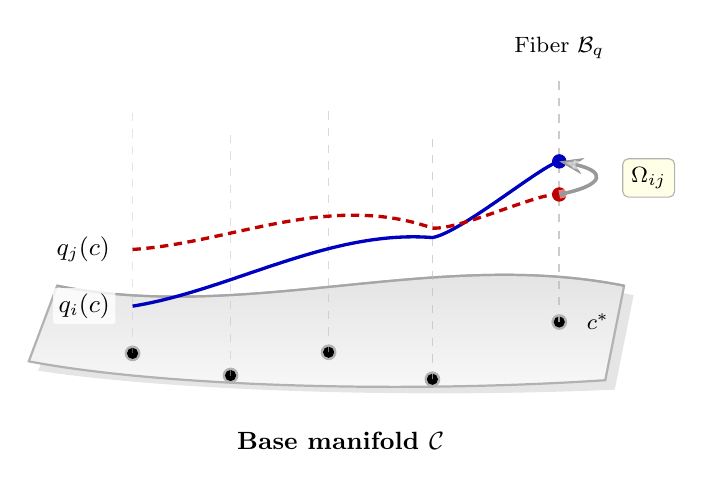
\begin{tikzpicture}[scale=1.2, every node/.style={font=\small}]
% requires \usetikzlibrary{calc, arrows.meta, decorations.markings, shadows}

% ------------------------------------------------------------------
% ENHANCED 3D BASE MANIFOLD with gradient and shadow
% ------------------------------------------------------------------
\path
  (0,0) coordinate (M1)
  (6,0) coordinate (M2)
  (5.8,-1.0) coordinate (M3)
  (-0.3,-0.8) coordinate (M4);

% Shadow layer
\filldraw[fill=black!10, draw=none]
  ($(M1)+(0.1,-0.1)$)
    .. controls (2.1,-0.5) and (4.1,0.3) .. ($(M2)+(0.1,-0.1)$)
    -- ($(M3)+(0.1,-0.1)$)
    .. controls (3.6,-1.2) and (1.1,-1.1) .. ($(M4)+(0.1,-0.1)$)
    -- cycle;

% Main surface with gradient
\shade[top color=gray!25, bottom color=gray!5, draw=gray!60, thick]
  (M1)
    .. controls (2,-0.4) and (4,0.4) .. (M2)
    -- (M3)
    .. controls (3.5,-1.15) and (1.0,-1.05) .. (M4)
    -- cycle;

% Surface outline for crispness
\draw[gray!70, thick]
  (M1)
    .. controls (2,-0.4) and (4,0.4) .. (M2);

\node[below, black, font=\small\bfseries] at (3,-1.45) {Base manifold $\mathcal{C}$};

% ------------------------------------------------------------------
% FIBER ANCHOR POINTS with improved positioning
% ------------------------------------------------------------------
\coordinate (C1) at ($(M4)!0.18!(M3)+(0,0.12)$);
\coordinate (C2) at ($(M4)!0.35!(M3)+(0,-0.08)$);
\coordinate (C3) at ($(M4)!0.52!(M3)+(0,0.20)$);
\coordinate (C4) at ($(M4)!0.70!(M3)+(0,-0.05)$);
\coordinate (C5) at ($(M4)!0.92!(M3)+(0,0.60)$);

% Anchor points with subtle glow
\foreach \c in {C1,C2,C3,C4,C5} {
  \filldraw[black!30] (\c) circle (2.2pt);
  \filldraw[black] (\c) circle (1.5pt);
}

% ------------------------------------------------------------------
% FIBERS with gradient opacity for depth
% ------------------------------------------------------------------
\foreach \c [count=\i] in {C1,C2,C3,C4,C5} {
  \pgfmathsetmacro{\opacity}{0.3 + \i*0.1}
  \draw[gray!50, dashed, line width=0.6pt, opacity=\opacity] 
    (\c) -- ++(0,2.6);
}

% Fiber label with better positioning
\node[above=3pt, black, font=\footnotesize] at ($(C5)+(0,2.6)$) {Fiber $\mathcal{B}_q$};

% ------------------------------------------------------------------
% SECTION CURVES with enhanced styling
% ------------------------------------------------------------------
% Section q_i (solid blue)
\draw[thick, blue!75!black, line width=1.2pt]
  ($(C1)+(0,0.5)$)
    .. controls ($(C2)+(0,0.9)$) and ($(C3)+(0,1.3)$)
    .. ($(C4)+(0,1.5)$)
    .. controls ($(C4)+(0.3,1.55)$) and ($(C5)+(-0.2,1.65)$)
    .. ($(C5)+(0,1.7)$);

% Section q_j (dashed red)
\draw[thick, red!75!black, densely dashed, line width=1.2pt]
  ($(C1)+(0,1.1)$)
    .. controls ($(C2)+(0,1.4)$) and ($(C3)+(0,1.7)$)
    .. ($(C4)+(0,1.6)$)
    .. controls ($(C4)+(0.3,1.58)$) and ($(C5)+(-0.2,1.38)$)
    .. ($(C5)+(0,1.35)$);

% Enhanced section labels with background
\node[left=6pt, black, fill=white, fill opacity=0.8, text opacity=1, 
      inner sep=2pt, rounded corners=1pt] 
  at ($(C1)+(0,0.5)$) {$q_i(c)$};
\node[left=6pt, black, fill=white, fill opacity=0.8, text opacity=1, 
      inner sep=2pt, rounded corners=1pt] 
  at ($(C1)+(0,1.1)$) {$q_j(c)$};

% Section endpoint markers
\filldraw[blue!75!black] ($(C5)+(0,1.7)$) circle (2pt);
\filldraw[red!75!black]  ($(C5)+(0,1.35)$) circle (2pt);

% Highlight the special point c*
\node[right=3pt, black, font=\footnotesize\itshape] 
  at ($(C5)+(0.1,0)$) {$c^*$};

% ------------------------------------------------------------------
% TRANSPORT OPERATOR with improved arrow
% ------------------------------------------------------------------
\draw[-{Stealth[length=3mm, width=2mm]}, very thick, black!80, 
      line width=1.3pt,
      postaction={draw, line width=3pt, white, opacity=0.5, -{Stealth[length=3mm, width=2mm]}}]
  ($(C5)+(0,1.35)$)
    .. controls ($(C5)+(0.5,1.45)$) and ($(C5)+(0.5,1.60)$)
    .. ($(C5)+(0,1.7)$);

% Transport label with background box
\node[right=5pt, black, fill=yellow!10, draw=black!30, 
      inner sep=3pt, rounded corners=2pt, font=\footnotesize\bfseries] 
  at ($(C5)+(0.52,1.525)$) {$\Omega_{ij}$};

\end{tikzpicture}
\caption{%
Visualization of agent sections $q_i(c)$ and $q_j(c)$ over an associated bundle. 
The shaded surface represents the base manifold $\mathcal{C}$, with vertical fibers $\mathcal{B}_q$ 
shown as dashed lines anchored at black points. 
At the reference point $c^*$ on the rightmost fiber, the transport operator $\Omega_{ij}(c^*)$ 
maps the red section value $q_j(c^*)$ into the blue section value $q_i(c^*)$, 
enabling frame alignment between agent representations.
}
\label{fig:bundle_sections_surface}
\end{figure}


\section{Methods}

We begin with a general geometric construction that naturally supports hierarchical emergence of meta-agents, scale interactions, and non-trivial holonomy of transport. The details of the most general geometry and framework can be found in the appendix and references \citep{nakahara2003geometry,kullback1951information,sternberg1994group,fulton1991representation,frankel2011geometry,baez1994gauge}.  Briefly, in this current report, we describe agents as modeled by a local section of an associated bundle to a principal $G$ fiber bundle. This framework enables a unified description of both intra-agent inference and inter-agent communication in terms of gauge frame transport and alignment.

\subsection{Code Availability}
The complete simulation suite that implements the gauge-theoretic variational inference framework described in this work is publicly available at 
\begin{itemize}
\item \href{https://github.com/cdenn016/epistemic-geometry}{https://github.com/cdenn016/epistemic-geometry}. 
\end{itemize}


All experiments reported in the results section can be reproduced using the provided configuration files and random number generator seeds documented in the repository. The codebase requires Python 3.9+ with NumPy, SciPy, and Joblib dependencies as specified in \texttt{requirements.txt}.

\subsection{Specializations for the Current Study}
Here we specify the simplifications adopted for the remainder of this work, which retain essential geometric structure while ensuring computational tractability and simplification.

\subsubsection{Matched Bundles}
In our general formulation agents are treated as pairs of sections of associated bundles $\mathcal{B}_q$ and $\mathcal{B}_p$ of beliefs and models.  Here we simplify by implementing

\begin{equation}
\mathcal{B}_q = \mathcal{B}_p =: \mathcal{B}, \qquad \rho_q = \rho_p =: \rho.
\end{equation}

This gives $\mathcal{E}_q = \mathcal{E}_p =: \mathcal{E}$, and the bundle morphisms become:

\begin{equation}
\Phi = \tilde{\Phi} = \text{id}_{\mathcal{E}}.
\end{equation}

Each agent then reduces to a single section $\sigma^i: \mathcal{U}_i \to \mathcal{E}$, with belief/prior distinction maintained through local fiber coordinates.



\subsubsection{Gauge Group and Representations}
The natural gauge group for KL-based attention is $G = \mathrm{GL}(K)$, the general linear group of invertible $K \times K$ matrices. This acts on the fibers via representations:

\begin{equation}
\rho_q: \mathrm{GL}(K) \to \mathrm{GL}(d_q),
\qquad
\rho_p: \mathrm{GL}(K) \to \mathrm{GL}(d_p).
\label{eq:representations}
\end{equation}

For $\Omega \in \mathrm{GL}(K)$, the gauge action on a Gaussian state is:

\begin{equation}
\boxed{
\begin{aligned}
\rho_q(\Omega) \cdot (\mu_q, \Sigma_q)
&= \big(\rho_q(\Omega)\,\mu_q,\;
\rho_q(\Omega)\,\Sigma_q\,\rho_q(\Omega)^\top\big),\\
\rho_p(\Omega) \cdot (\mu_p, \Sigma_p)
&= \big(\rho_p(\Omega)\,\mu_p,\;
\rho_p(\Omega)\,\Sigma_p\,\rho_p(\Omega)^\top\big).
\end{aligned}
}
\label{eq:gauge_action_gaussians}
\end{equation}

By Theorem~\ref{thm:glk_invariance}, KL divergence is invariant under this action for any $\Omega \in \mathrm{GL}(K)$. The only requirement is invertibility ($\det \Omega \neq 0$), not orthogonality.







\begin{table}[h]
\centering
\renewcommand{\arraystretch}{1.2}
\setlength{\tabcolsep}{6pt}
\begin{tabularx}{\textwidth}{lXX}
\hline
\textbf{Property} &
\textbf{Full Gauge Theory} &
\textbf{Standard Transformer} \\
\hline
Gauge group $G$ &
$\mathrm{GL}(K)$ or subgroup &
$\mathrm{GL}(d_k)$ (implicit) \\
Gauge transformation &
$\Omega_{ij} = e^{\phi_i} e^{-\phi_j}$ &
$\Omega = W_Q W_K^\top$ (learned, constant) \\
Frame field $\phi_i(c)$ &
Varies per agent/position &
Absorbed into $W_Q, W_K$ \\
Transport structure &
Agent-pair dependent &
Uniform across all pairs \\
Connection $A_\mu$ &
$-\partial_\mu \phi_i \neq 0$ &
$0$ (flat connection) \\
Curvature $F_{\mu\nu}$ &
Can be $\neq 0$ &
$0$ (trivial holonomy) \\
KL coupling &
$D_{\text{KL}}[q_i \,\|\, \Omega_{ij} q_j]$ &
$D_{\text{KL}}[q_i \,\|\, \Omega q_j]$ with constant $\Omega$ \\
What is learned &
Frame fields $\phi_i$ &
Global gauge $W_Q, W_K$ \\
\hline
\end{tabularx}
\caption{Comparison between full gauge-theoretic formulation and standard transformers.}
\label{tab:gauge_vs_transformer}
\end{table}





\subsubsection{Local Gauge Frames}
Each agent $i$ has a gauge frame field $\phi_i: \mathcal{U}_i \to \mathfrak{gl}(K)$ which may vary spatially.  This induces a local connection:

\begin{equation}
A^{(i)}_\mu(c) = -\partial_\mu \phi_i(c) + \mathcal{O}(\phi_i^2),
\end{equation}

with field strength:

\begin{equation}
F^{(i)}_{\mu\nu}(c) = \partial_\mu A^{(i)}_\nu - \partial_\nu A^{(i)}_\mu + [A^{(i)}_\mu, A^{(i)}_\nu].
\end{equation}


\subsubsection{0D Base Manifold}

In order to connect the gauge theory to transformer architectures we consider the case of a 0-dimensional base manifold. Agents occupy a single point and overlap with each other completely. However, the full theory is extensible to arbitrary smooth base manifolds.

Since we are considering 0-dimensional base manifolds there exist no gauge connections or field strengths simplifying the geometry considerably.




\subsubsection{Gauge-Aligned Divergence}
With these assumptions, the gauge-aligned KL divergence between agents is (see appendix):

\begin{equation}
D_{\text{KL}}\left[q_i(c) \,\big\|\, \Omega_{ij}(c) q_j(c)\right],
\end{equation}

where for Gaussian beliefs:

\begin{equation}
\Omega_{ij}(c) \cdot (\mu_j, \Sigma_j) = \left(\Omega_{ij}(c)\mu_j, \, \Omega_{ij}(c)\Sigma_j\Omega_{ij}(c)^\top\right).
\end{equation}

This divergence forms the basis of our attention mechanism.

\subsubsection{$\mathrm{GL}(K)$ Gauge Invariance of KL Divergence}
\label{sec:glk_invariance}

A crucial observation underlying our framework is that the Kullback-Leibler divergence possesses a maximal gauge symmetry: it is invariant under the full general linear group $\mathrm{GL}(K)$, not merely orthogonal subgroups. This is a standard result in information geometry (see, e.g., \citet{amari2016information}), but its implications for transformer attention have not been previously recognized. We state it here for completeness.

\begin{theorem}[$\mathrm{GL}(K)$ Gauge Invariance]
\label{thm:glk_invariance}
For any two Gaussian distributions $P = \mathcal{N}(\mu_P, \Sigma_P)$ and $Q = \mathcal{N}(\mu_Q, \Sigma_Q)$ on $\mathbb{R}^K$, and any invertible linear transformation $\Omega \in \mathrm{GL}(K)$, the KL divergence is invariant under simultaneous pushforward:
\begin{equation}
D_{\mathrm{KL}}(\Omega_* P \,\|\, \Omega_* Q) = D_{\mathrm{KL}}(P \,\|\, Q),
\label{eq:glk_invariance}
\end{equation}
where $\Omega_* P = \mathcal{N}(\Omega\mu_P, \Omega\Sigma_P\Omega^\top)$ denotes the pushforward of $P$ under $\Omega$.
\end{theorem}

\begin{proof}
The KL divergence between Gaussians consists of three terms:
\begin{equation}
D_{\mathrm{KL}}(P \| Q) = \frac{1}{2}\left[\mathrm{Tr}(\Sigma_Q^{-1}\Sigma_P) + (\mu_P - \mu_Q)^\top \Sigma_Q^{-1}(\mu_P - \mu_Q) - K + \log\frac{\det\Sigma_Q}{\det\Sigma_P}\right].
\end{equation}

Under the pushforward $\Omega_* P = \mathcal{N}(\Omega\mu_P, \Omega\Sigma_P\Omega^\top)$ and $\Omega_* Q = \mathcal{N}(\Omega\mu_Q, \Omega\Sigma_Q\Omega^\top)$:

\textbf{Trace term:}
\begin{equation}
\mathrm{Tr}\big[(\Omega\Sigma_Q\Omega^\top)^{-1}(\Omega\Sigma_P\Omega^\top)\big] = \mathrm{Tr}\big[\Omega^{-\top}\Sigma_Q^{-1}\Omega^{-1}\Omega\Sigma_P\Omega^\top\big] = \mathrm{Tr}(\Sigma_Q^{-1}\Sigma_P). \quad \checkmark
\end{equation}

\textbf{Quadratic term:}
\begin{align}
&(\Omega\mu_P - \Omega\mu_Q)^\top (\Omega\Sigma_Q\Omega^\top)^{-1} (\Omega\mu_P - \Omega\mu_Q) \nonumber\\
&= (\mu_P - \mu_Q)^\top \Omega^\top \Omega^{-\top}\Sigma_Q^{-1}\Omega^{-1}\Omega (\mu_P - \mu_Q) = (\mu_P - \mu_Q)^\top \Sigma_Q^{-1}(\mu_P - \mu_Q). \quad \checkmark
\end{align}

\textbf{Log-determinant term:}
\begin{equation}
\log\frac{\det(\Omega\Sigma_Q\Omega^\top)}{\det(\Omega\Sigma_P\Omega^\top)} = \log\frac{(\det\Omega)^2 \det\Sigma_Q}{(\det\Omega)^2 \det\Sigma_P} = \log\frac{\det\Sigma_Q}{\det\Sigma_P}. \quad \checkmark
\end{equation}

The $(\det\Omega)^2$ factors cancel identically. Since all three components are invariant, $D_{\mathrm{KL}}(\Omega_* P \| \Omega_* Q) = D_{\mathrm{KL}}(P \| Q)$.
\end{proof}

This invariance has several important implications for our framework:

\begin{enumerate}
\item \textbf{Maximal gauge symmetry}: The natural gauge group for KL-based attention is $\mathrm{GL}(K)$. 

\item \textbf{Generalization to $f$-divergences}: The proof extends to all $f$-divergences. For any convex function $f$ with $f(1) = 0$:
\begin{equation}
D_f(\Omega_* P \| \Omega_* Q) = D_f(P \| Q), \quad \forall\, \Omega \in \mathrm{GL}(K).
\end{equation}
The Jacobian factors $|\det\Omega|$ from the density transformation cancel in the ratio $p(x)/q(x)$.

\item \textbf{Simplified implementation}: Transport operators need only satisfy $\det(\Omega_{ij}) \neq 0$ (invertibility), not $\Omega_{ij}^\top\Omega_{ij} = I$ (orthogonality). This eliminates the need for computationally expensive re-orthogonalization procedures.

\item \textbf{Learned projections as gauge transformations}: As we shall demonstrate, the query and key projection matrices $W_Q, W_K \in \mathrm{GL}(d_k)$ in standard transformers are themselves gauge transformations. The "constant gauge limit" corresponds not to the absence of gauge structure, but to a constant gauge transformation $\Omega = W_Q W_K^\top$ applied uniformly across all token pairs.
\end{enumerate}

The $\mathrm{GL}(K)$ invariance reveals that the attention mechanism respects a form of general covariance: the information-geometric distance between beliefs is independent of the coordinate system (basis) used to represent them. This is the statistical analogue of coordinate independence in differential geometry.

\begin{table}[h]
\centering
\renewcommand{\arraystretch}{1.15}
\setlength{\tabcolsep}{6pt}
\begin{tabularx}{\textwidth}{l>{\raggedright\arraybackslash}Xl}
\hline
\textbf{Symbol} & \textbf{Description} & \textbf{Type/Dimension} \\
\hline
\multicolumn{3}{l}{\textit{Fiber Bundle Structure}} \\
$\mathcal{M}$ & Base manifold (spatial domain) & Manifold \\
$Q_i$ & Belief fiber at agent $i$ & $\mathbb{R}^{K_q}$ \\
$P_i$ & Model fiber at agent $i$ & $\mathbb{R}^{K_p}$ \\
$G$ & Gauge group & $\mathrm{GL}(K)$ \\
$\mathfrak{g}$ & Lie algebra of $G$ & $\mathfrak{gl}(K)$ \\
\\
\multicolumn{3}{l}{\textit{Gauge Fields and Connections}} \\
$\Omega^q_{ij}$ & Connection $Q_j \to Q_i$ & $\mathrm{GL}(K_q)$ \\
$\Omega^p_{ij}$ & Connection $P_j \to P_i$ & $\mathrm{GL}(K_p)$ \\
$\phi_i$ & Gauge parameter (belief frame) & $\mathfrak{g}\!\cong\!\mathbb{R}^3$ \\
$\tilde{\phi}_i$ & Gauge parameter (model frame) & $\mathfrak{g}\!\cong\!\mathbb{R}^3$ \\
$A_\mu(x)$ & Gauge connection field & $\mathfrak{g}$-valued 1-form \\
\\
\multicolumn{3}{l}{\textit{Bundle Morphisms}} \\
$\Phi_i$ & Morphism $Q_i \to P_i$ & $\mathbb{R}^{K_p\times K_q}$ \\
$\tilde{\Phi}_i$ & Morphism $P_i \to Q_i$ & $\mathbb{R}^{K_q\times K_p}$ \\
\\
\multicolumn{3}{l}{\textit{Statistical Parameters}} \\
$q_i(k_i)$ & Belief distribution & $\mathcal{N}(\mu_{q,i},\Sigma_{q,i})$ \\
$p_i(k_i)$ & Model distribution & $\mathcal{N}(\mu_{p,i},\Sigma_{p,i})$ \\
$\mu_{q,i},\mu_{p,i}$ & Mean vectors & $\mathbb{R}^{K_q},\mathbb{R}^{K_p}$ \\
$\Sigma_{q,i},\Sigma_{p,i}$ & Covariance matrices & $\mathbb{R}^{K\times K},\succ0$ \\
\\
\multicolumn{3}{l}{\textit{Attention and Coupling}} \\
$\beta_{ij}$ & Attention weight $j\!\to\!i$ & $[0,1]$ \\
$\tau$ & Attention temperature & $\mathbb{R}_+$ \\
$\alpha$ & Self-consistency strength & $\mathbb{R}_+$ \\
$D_{\mathrm{KL}}$ & Kullback–Leibler divergence & $\mathbb{R}_+\cup\{0\}$ \\
\hline
\end{tabularx}
\caption{Principal notation used throughout this paper.}
\label{tab:notation}
\end{table}



The full geometric framework admits considerable generalization: path-dependent parallel transport with holonomy effects, non-flat gauge connections exhibiting epistemic monopoles, curved base manifolds such as hyperbolic or spherical latent spaces, heterogeneous fiber structures where $\mathcal{B}_q \neq \mathcal{B}_p$, cross-scale dynamics with meta-agent emergence, curvature-induced phase transitions in multi-agent systems, and pullback geometries via agent sections from informational fibers to the base manifold.


\section{Derivation of Generalized Variational Free Energy from a Normalized Generative Model}
We derive the generalized variational free energy we will utilize from general first principles, showing that both belief alignment (weighted by $\beta_{ij}$) and model alignment (weighted by $\gamma_{ij}$) emerge naturally from a single normalized generative prior with auxiliary agreement variables. This construction justifies the KL-based coupling terms as consequences of gauge-transported Gaussian consistency constraints. In what follows we shall assume all probability distributions are defined at a specific base manifold point $c = c^*$ unless otherwise noted.  We will label the fiber's latent coordinates as $k_i \in \mathcal{B}$ in order to define the necessary integrals

\subsection{Setup}
\subsubsection{Latent Variables and Fiber Geometry}
Each agent $i$ maintains two distinct latent variables living in separate fiber bundles:

\begin{equation}
k_i \in \mathbb{R}^{d_q} \quad \text{(belief latent in $\mathcal{E}_q$)}, 
\qquad
m_i \in \mathbb{R}^{d_p} \quad \text{(model latent in $\mathcal{E}_p$)}.
\label{eq:dual_latents}
\end{equation}

The full state of agent $i$ at base manifold point $c^*$ is a Gaussian distribution over each latent:

\begin{equation}
\begin{aligned}
q_i(k_i) &= \mathcal{N}(k_i\,;\mu_{q,i},\,\Sigma_{q,i}), 
\quad \mu_{q,i} \in \mathbb{R}^{d_q},\; 
\Sigma_{q,i} \in \mathbb{R}^{d_q \times d_q}, \; \Sigma_{q,i} \succ 0,\\
s_i(m_i) &= \mathcal{N}(m_i\,;\mu_{p,i},\,\Sigma_{p,i}), 
\quad \mu_{p,i} \in \mathbb{R}^{d_p},\; 
\Sigma_{p,i} \in \mathbb{R}^{d_p \times d_p}, \; \Sigma_{p,i} \succ 0.
\end{aligned}
\label{eq:gaussian_states}
\end{equation}

Thus, the fiber at each agent's location $c \in \mathcal{C}$ is the product statistical manifold:

\begin{equation}
\mathcal{B}(c) = \mathcal{B}_q \times \mathcal{B}_p,
\label{eq:fiber_product}
\end{equation}

where

\begin{equation}
\begin{aligned}
\mathcal{B}_q &= \left\{
(\mu_q, \Sigma_q) : 
\mu_q \in \mathbb{R}^{d_q}, \;
\Sigma_q \in \mathbb{R}^{d_q \times d_q}, \;
\Sigma_q \succ 0
\right\},\\
\mathcal{B}_p &= \left\{
(\mu_p, \Sigma_p) : 
\mu_p \in \mathbb{R}^{d_p}, \;
\Sigma_p \in \mathbb{R}^{d_p \times d_p}, \;
\Sigma_p \succ 0
\right\}.
\end{aligned}
\label{eq:statistical_manifolds}
\end{equation}

\subsection{Base Priors}
Each latent has an independent Gaussian base prior encoding agent-specific inductive biases:

\begin{equation}
p_i(k_i) = \mathcal{N}(k_i\,; \mu_{0,i}^{(q)}, \Sigma_{0,i}^{(q)}), 
\qquad
r_i(m_i) = \mathcal{N}(m_i\,; \mu_{0,i}^{(p)}, \Sigma_{0,i}^{(p)}).
\label{eq:base_priors}
\end{equation}

These priors are \textbf{local}—they live in each agent's own gauge frame and need not be related across agents until transported via $\Omega_{ij}$.

\subsubsection{Auxiliary Agreement Variables}
To enforce consistency between agents after gauge transport, we introduce an auxiliary "agreement" variable for each ordered pair $(i,j)$:

\begin{equation}
z_{ij} \in \mathbb{R}^{d_q} \quad \text{(belief agreement)}, 
\qquad
w_{ij} \in \mathbb{R}^{d_p} \quad \text{(model agreement)}.
\label{eq:agreement_vars}
\end{equation}

\begin{itemize}
  \item $z_{ij}$: "What agent $i$ believes agent $j$'s belief looks like, after transporting $j$'s belief into $i$'s gauge frame"
  \item $w_{ij}$: "What agent $i$ believes agent $j$'s generative model looks like, after gauge transport"
\end{itemize}

These will be latent mediators that will be integrated out, leaving an effective pairwise coupling between $k_i, k_j$ and $m_i, m_j$.

Agreement variables provide a convenient parameterization of the joint generative model. As shown in Section~\ref{sec:marginal_mrf}, integrating out the auxiliary variables yields a pairwise Markov random field with gauge-covariant potentials and a partition function $Z$. The auxiliary variable representation offers computational advantages for certain inference procedures, though it does not eliminate the partition function.

\subsection{Normalized Joint Generative Model}
We define the Gaussian couplings and enforce that each agreement variable $z_{ij}$,$w_{ij}$ simultaneously matches:

\begin{enumerate}
  \item Agent $i$'s own latent $k_i$, $m_i$
  \item Agent $j$'s latent $k_j$, $m_j$ after gauge transport into agent $i$'s frame
\end{enumerate}

The auxiliary variable $z_{ij}$ is drawn from the product of Gaussians:

\begin{equation}
p(z_{ij} \mid k_i, k_j) \propto 
\mathcal{N}(z_{ij}; k_i, \Lambda_{ij}^{-1}) \cdot 
\mathcal{N}(z_{ij}; \Omega_{ij}k_j, \Lambda_{ij}^{-1})
\label{eq:belief_coupling_product}
\end{equation}

and similarly for model alignment:

\begin{equation}
p(w_{ij} \mid m_i, m_j) \propto 
\mathcal{N}(w_{ij}; m_i, \Gamma_{ij}^{-1}) \cdot 
\mathcal{N}(w_{ij}; \tilde{\Omega}_{ij}m_j, \Gamma_{ij}^{-1})
\label{eq:model_coupling_product}
\end{equation}

where:

\begin{itemize}
  \item $\Lambda_{ij} \in \mathbb{R}^{d_q \times d_q}$, $\Lambda_{ij} \succ 0$: Belief alignment precision
  \item $\Gamma_{ij} \in \mathbb{R}^{d_p \times d_p}$, $\Gamma_{ij} \succ 0$: Model alignment precision
  \item $\Omega_{ij} \in \mathrm{GL}(K)$: Gauge transport from agent $j$'s frame to agent $i$'s frame (belief channel)
  \item $\tilde{\Omega}_{ij} \in \mathrm{GL}(K)$: Gauge transport from agent $j$'s frame to agent $i$'s frame (model channel)
\end{itemize}

\subsubsection{Gauge Transport as Frame Transformation}
The gauge transport operators $\Omega_{ij}, \tilde{\Omega}_{ij}$ are not parallel transport along a connection in the usual sense (which would be path-dependent). Instead, they are pointwise gauge frame transformations:

\begin{equation}
\Omega_{ij}(c) = e^{\phi_i(c)} \cdot e^{-\phi_j(c)} \in \mathrm{GL}(K),
\label{eq:gauge_frame_rotation}
\end{equation}

where $\phi_i: \mathcal{U}_i \to \mathfrak{gl}(K)$ is agent $i$'s gauge frame field (a local section of the Lie algebra bundle).

These act on the latent variables as

\begin{equation}
\begin{aligned}
\Omega_{ij} k_j
&:= \rho_q(\Omega_{ij}) \, k_j
\in \mathbb{R}^{d_q},\\
\tilde{\Omega}_{ij} m_j
&:= \rho_p(\tilde{\Omega}_{ij}) \, m_j
\in \mathbb{R}^{d_p}.
\end{aligned}
\label{eq:gauge_action_on_vectors}
\end{equation}

In the transformer limit, $\Omega_{ij} = \Omega = W_Q W_K^\top$ becomes a constant learned gauge transformation (see Section~\ref{sec:wq_wk_gauge}).

\subsubsection{Full Joint Distribution}
The joint generative model over all latents and auxiliary variables is:

\begin{equation}
\boxed{
\begin{aligned}
p&(\{k_i\},\{m_i\},\{z_{ij}\},\{w_{ij}\})\\
&=\left[\prod_i p_i(k_i)\,r_i(m_i)\right]\\
&\quad\times
\left[\prod_{i,j}
\mathcal{N}(z_{ij}\,;k_i,\Lambda_{ij}^{-1})
\,\mathcal{N}(z_{ij}\,;\Omega_{ij}k_j,\Lambda_{ij}^{-1})\right]\\
&\quad\times
\left[\prod_{i,j}
\mathcal{N}(w_{ij}\,;m_i,\Gamma_{ij}^{-1})
\,\mathcal{N}(w_{ij}\,;\tilde{\Omega}_{ij}m_j,\Gamma_{ij}^{-1})\right].
\end{aligned}
}
\label{eq:joint_distribution}
\end{equation}

\subsubsection{Marginal Structure and Partition Function}
\label{sec:marginal_mrf}

The product of two Gaussians in the auxiliary variable $z_{ij}$ yields
\begin{equation}
\mathcal{N}(z_{ij};k_i,\Lambda_{ij}^{-1})\,\mathcal{N}(z_{ij};\Omega_{ij}k_j,\Lambda_{ij}^{-1})
= C_{ij}(k_i,k_j)\;\mathcal{N}\!\left(z_{ij};\tfrac{k_i+\Omega_{ij}k_j}{2},\tfrac{\Lambda_{ij}^{-1}}{2}\right),
\end{equation}
where the coupling factor is
\begin{equation}
C_{ij}(k_i,k_j) \propto \exp\!\left(-\tfrac{\Lambda_{ij}}{4}\|k_i - \Omega_{ij}k_j\|^2\right).
\end{equation}
Integrating out the auxiliary variables, the marginal over primary latents takes the form of a pairwise Markov random field:
\begin{equation}
p(\{k_i\},\{m_i\}) = \frac{1}{Z}\prod_i p_i(k_i)\,r_i(m_i)
\prod_{i,j} \exp\!\left(-\tfrac{\Lambda_{ij}}{4}\|k_i - \Omega_{ij}k_j\|^2\right)
\exp\!\left(-\tfrac{\Gamma_{ij}}{4}\|m_i - \tilde{\Omega}_{ij}m_j\|^2\right),
\label{eq:marginal_mrf}
\end{equation}
with partition function $Z$. The auxiliary variable representation \eqref{eq:joint_distribution} provides a convenient parameterization, but does not eliminate the partition function. For variational inference, explicit computation of $Z$ is unnecessary: the variational free energy depends only on expectations under the factorized posterior, not on the normalizing constant of the prior.
\subsection{Variational Free Energy}
We now form the variational free energy under a mean-field posterior approximation. Assume a factorized posterior
\begin{equation}
q(\{k_i\},\{m_i\})=\prod_i q_i(k_i)\,s_i(m_i),
\label{eq:mean_field_posterior}
\end{equation}
with Gaussian factors
\begin{equation}
q_i(k_i)=\mathcal{N}(k_i;\mu_{q,i},\Sigma_{q,i}),
\qquad
s_i(m_i)=\mathcal{N}(m_i;\mu_{p,i},\Sigma_{p,i}).
\label{eq:gaussian_factors}
\end{equation}
The variational free energy is defined as
\begin{equation}
\mathcal{F}
:=\mathbb{E}_q[\log q(\{k_i\},\{m_i\})]
-\mathbb{E}_q[\log p(\{k_i\},\{m_i\})]
-\mathbb{E}_q[\log p(o\,|\{k_i\},\{m_i\})],
\label{eq:free_energy_definition}
\end{equation}
where $p(o\,|\{k_i\},\{m_i\})$ is the observation likelihood \citep{friston2010free,parr2022active}.

Expanding the first two terms using \eqref{eq:mean_field_posterior} and the marginal prior, and dropping additive constants, we obtain
\begin{equation}
\begin{aligned}
\mathcal{F}
&=\sum_i D_{\mathrm{KL}}(q_i\,\|\,p_i)
+\sum_i D_{\mathrm{KL}}(s_i\,\|\,r_i)\\
&\quad+\frac{1}{4}\sum_{i,j}\mathbb{E}_{q_i q_j}
\!\big[(k_i-\Omega_{ij}k_j)^\top\Lambda_{ij}(k_i-\Omega_{ij}k_j)
\big]\\
&\quad+\frac{1}{4}\sum_{i,j}\mathbb{E}_{s_i s_j}
\!\big[(m_i-\tilde{\Omega}_{ij}m_j)^\top\Gamma_{ij}(m_i-\tilde{\Omega}_{ij}m_j)
\big]\\
&\quad-\mathbb{E}_q[\log p(o\,|\{k_i\},\{m_i\})].
\end{aligned}
\label{eq:free_energy_expanded}
\end{equation}
The first two lines contain single-agent KL divergences from base priors. The third and fourth lines contain pairwise quadratic forms encoding the agent-agent alignment. The final term is the negative log-likelihood of observations.

\section{Relating The Quadratic Forms to Transported KL Divergences}
We now show that the pairwise quadratic expectations in \eqref{eq:free_energy_expanded} can be expressed in terms of KL divergences between transported distributions (see appendix for general requirement of the forward KL).
\subsection{Exact expansion for Gaussian beliefs}
For independent Gaussians $q_i = \mathcal{N}(\mu_{q,i},\Sigma_{q,i})$ and $q_j = \mathcal{N}(\mu_{q,j},\Sigma_{q,j})$, the expectation of a quadratic form is
\begin{equation}
\mathbb{E}_{q_i q_j}[\delta^\top A \delta]
= \mathrm{tr}\!\big(A\,\mathrm{Cov}(\delta)\big)
+ \bar{\delta}^\top A \bar{\delta},
\label{eq:quadratic_expectation_formula}
\end{equation}
where $\delta = k_i - \Omega_{ij}k_j$, $\bar{\delta} = \mathbb{E}[\delta] = \mu_{q,i} - \Omega_{ij}\mu_{q,j}$, and
\begin{equation}
\mathrm{Cov}(\delta) = \Sigma_{q,i} + \Omega_{ij}\Sigma_{q,j}\Omega_{ij}^\top.
\label{eq:delta_covariance}
\end{equation}
Applying \eqref{eq:quadratic_expectation_formula} with $A = \Lambda_{ij}$:
\begin{equation}
\begin{aligned}
\mathbb{E}_{q_i q_j}
[(k_i-\Omega_{ij}k_j)^\top\Lambda_{ij}(k_i-\Omega_{ij}k_j)]
&=\mathrm{tr}\!\big[\Lambda_{ij}(\Sigma_{q,i}+\Omega_{ij}\Sigma_{q,j}\Omega_{ij}^\top)\big]\\
&\quad+(\mu_{q,i}-\Omega_{ij}\mu_{q,j})^\top
\Lambda_{ij}
(\mu_{q,i}-\Omega_{ij}\mu_{q,j}).
\end{aligned}
\label{eq:belief_quadratic_expansion}
\end{equation}
An identical expansion holds for the model channel with $\Gamma_{ij}$ and $\tilde{\Omega}_{ij}$.

We observe that a natural choice of coupling precisions $\Lambda_{ij}$ and $\Gamma_{ij}$ makes \eqref{eq:belief_quadratic_expansion} proportional to a KL divergence.

Specifically, we define
\begin{equation}
\Lambda_{ij}:=\tau^{(q)}_{ij}\,(\Omega_{ij}\Sigma_{q,j}\Omega_{ij}^\top)^{-1},
\qquad
\Gamma_{ij}:=\tau^{(p)}_{ij}\,(\tilde{\Omega}_{ij}\Sigma_{p,j}\tilde{\Omega}_{ij}^\top)^{-1},
\label{eq:precision_choice}
\end{equation}
where $\tau^{(q)}_{ij}, \tau^{(p)}_{ij} > 0$ are dimensionless coupling strengths.

\textbf{Remark.} This precision choice is a specific design decision within the framework, not the unique consequence of variational principles alone. Other choices of $\Lambda_{ij}$ (e.g., fixed identity, learned precision, or data-dependent) would yield different alignment functionals. The present choice is motivated by two considerations: (i) it produces a KL-divergence coupling, which is the unique $f$-divergence preserving exponential-family closure (see Appendix~C); and (ii) the resulting attention weights inherit the $\mathrm{GL}(K)$ invariance of the KL divergence (Theorem~\ref{thm:glk_invariance}). Alternative choices would break one or both of these properties.

Recall that the KL divergence between two Gaussians $q_i = \mathcal{N}(\mu_i,\Sigma_i)$ and $\Omega_{ij}q_j = \mathcal{N}(\Omega_{ij}\mu_j, \Omega_{ij}\Sigma_j\Omega_{ij}^\top)$ is
$$
D_{\mathrm{KL}}(q_i\,\|\,\Omega_{ij}q_j)
= \frac{1}{2}
\Big[
\mathrm{tr}\!\big((\Omega_{ij}\Sigma_j\Omega_{ij}^\top)^{-1}\Sigma_i\big)
- d_q
$$
$$
+ \log \frac{\det(\Omega_{ij}\Sigma_j\Omega_{ij}^\top)}{\det \Sigma_i}
+ (\mu_i - \Omega_{ij}\mu_j)^\top
(\Omega_{ij}\Sigma_j\Omega_{ij}^\top)^{-1}
(\mu_i - \Omega_{ij}\mu_j)
\Big].
\label{eq:kl_full}
$$
When beliefs are approximately aligned (the regime toward which the coupling drives the system at convergence), the covariances satisfy $\Sigma_i \approx \Omega_{ij}\Sigma_j\Omega_{ij}^\top$, and the trace and log-determinant terms approximately cancel. This approximation is self-consistent: the coupling promotes alignment, and the KL form is most accurate in the aligned regime. Early in training, when covariances may be far from aligned, the approximation introduces $O(\|\Delta\Sigma\|)$ errors that decrease as training proceeds. In this alignment regime, as shown in the appendix, the quadratic expectation becomes
\begin{equation}
\frac{1}{4}\mathbb{E}_{q_i q_j}
[(k_i-\Omega_{ij}k_j)^\top\Lambda_{ij}(k_i-\Omega_{ij}k_j)]
\approx
\frac{\tau^{(q)}_{ij}}{2}\,D_{\mathrm{KL}}(q_i\,\|\,\Omega_{ij}q_j)+\text{const},
\label{eq:belief_kl_relation}
\end{equation}
where the constant absorbs dimension-dependent terms and $O(\|\Delta\|^2)$ covariance mismatch corrections.

Similarly for the model channel:
\begin{equation}
\frac{1}{4}\mathbb{E}_{s_i s_j}
[(m_i-\tilde{\Omega}_{ij}m_j)^\top\Gamma_{ij}(m_i-\tilde{\Omega}_{ij}m_j)]
\approx
\frac{\tau^{(p)}_{ij}}{2}\,D_{\mathrm{KL}}(s_i\,\|\,\tilde{\Omega}_{ij}s_j)+\text{const}.
\label{eq:model_kl_relation}
\end{equation}
\subsection{Defining normalized alignment weights}
To obtain the standard form, we define normalized alignment weights
\begin{equation}
\beta_{ij}:=\frac{\tau^{(q)}_{ij}}{2},
\qquad
\gamma_{ij}:=\frac{\tau^{(p)}_{ij}}{2}.
\label{eq:normalized_weights}
\end{equation}
These weights have a clear interpretation: $\beta_{ij}$ measures the strength of belief alignment between agents $i$ and $j$, while $\gamma_{ij}$ measures model alignment strength. In the limit $\beta_{ij} \to \infty$ with fixed $\gamma_{ij}$, agents' beliefs are forced to perfect agreement after transport, while their models may still differ. Conversely, $\gamma_{ij} = 0$ decouples model alignment entirely. In all subsequent equations we take $\tau$ to be independent of each agent---a constant global value which we set to 1.



\subsection{Final Form of the Variational Free Energy}
\label{sec:final_free_energy}

Substituting and absorbing constants we arrive at the main result:
\begin{equation}
\boxed{
\begin{aligned}
\mathcal{F}[\{q_i\},\{s_i\}]
&=\sum_i D_{\mathrm{KL}}(q_i\,\|\,p_i)
+\sum_i D_{\mathrm{KL}}(s_i\,\|\,r_i)\\
&\quad+\sum_{i,j}\beta_{ij}\,D_{\mathrm{KL}}(q_i\,\|\,\Omega_{ij}q_j)\\
&\quad+\sum_{i,j}\gamma_{ij}\,D_{\mathrm{KL}}(s_i\,\|\,\tilde{\Omega}_{ij}s_j)\\
&\quad-\mathbb{E}_q[\log p(o\,|\{k_i\},\{m_i\})].
\end{aligned}
}
\label{eq:free_energy_final}
\end{equation}

\subsubsection{Simplified Variational Free Energy}
In our fiber-matched setting, the variational free energy for agent $i$ becomes (where, in the present study, we consider all agents to share the same generative models):
\begin{equation}
\mathcal{F}[q_i] = \int_{\mathcal{U}_i} \left[\alpha_i D_{\text{KL}}\left(q_i(c) \,\|\, p_i(c)\right) - \xi_i \mathbb{E}_{q_i(c)}\left[\log p_i(o_i \mid c)\right]\right] \mathrm{d}c,
\end{equation}
where both $q_i(c)$ and $p_i(c)$ are points in the same fiber $\mathcal{B}(c)$ and $\alpha_i$ and $\xi_i$ are parameters placed for full generality which we henceforth set equal to $1$.

We have shown that the cross-agent alignment term is the forward KL divergence with frame rotation:
\begin{equation}
\mathcal{F}_{\text{align}} = \sum_{i,j} \int_{\mathcal{U}_i \cap \mathcal{U}_j} \chi_{ij}(c) \, \beta_{ij}(c) \, D_{\text{KL}}\left(q_i(c) \,\big\|\, \Omega_{ij}(c) \cdot q_j(c)\right) \, \mathrm{d}c,
\end{equation}
where $\Omega_{ij}(c) \cdot q_j(c)$ denotes the gauge transport of agent $j$'s belief into agent $i$'s frame, and both operands live in the same statistical manifold $\mathcal{B}(c)$ (similarly for $p$).

The attention weights derived from this framework take the form:
\begin{equation}
\beta_{ij}(c) = \frac{\exp\left[-\frac{1}{\tau} D_{\text{KL}}\left(q_i(c) \,\big\|\, \Omega_{ij}(c) q_j(c)\right)\right] \chi_{ij}(c)}{\sum_k \exp\left[-\frac{1}{\tau} D_{\text{KL}}\left(q_i(c) \,\big\|\, \Omega_{ik}(c) q_k(c)\right)\right] \chi_{ik}(c)},
\end{equation}
where
$$
\chi_{ij}(c) = \mathbb{I}_{\mathcal{U}_i \cap \mathcal{U}_j}(c)
$$
is the overlap indicator, and $\tau$ is the inverse temperature parameter controlling attention sharpness.
\subsection{Interpretation}
Each term in the variational free energy \eqref{eq:free_energy_final} encodes a distinct aspect of multi-agent inference:

(1) Belief Prior: $D_{\mathrm{KL}}(q_i \| p_i)$

The belief prior measures the deviation of agent $i$'s current belief $q_i(k_i)$ from its local prior $p_i(k_i \mid m_i)$. This term regularizes beliefs toward locally expected states. In the absence of observations and inter-agent coupling, minimizing $\mathcal{F}$ would yield $q_i^* = p_i$, recovering pure prior-based prediction.

(2) Model Prior: $D_{\mathrm{KL}}(s_i \| r_i)$

The model prior, similarly measures the deviation of agent $i$'s current model belief $s_i(m_i)$ from its hyperprior $r_i(m_i)$. This term regularizes model beliefs toward baseline expectations. It prevents overfitting to recent data by anchoring $s_i$ to a stable hyperprior $r_i$ determined from some higher, slower level.

Hierarchical relationship to (1): The prior $p_i(k_i \mid m_i)$ in term (1) depends on the model parameters $m_i$ that are themselves uncertain under $s_i(m_i)$. Thus:
\begin{equation}
p_i(k_i) = \int p_i(k_i \mid m_i) \, s_i(m_i) \, \mathrm{d}m_i
\label{eq:hierarchical_prior}
\end{equation}
This creates a two-level Bayesian hierarchy: uncertainty about states ($q_i$) and uncertainty about the model generating those states ($s_i$).

(3) Belief Alignment: $\beta_{ij} D_{\mathrm{KL}}(q_i \| \Omega_{ij} q_j)$

Belief alignment represents the discrepancy between agent $i$'s belief and agent $j$'s belief after gauge transport into agent $i$'s local frame - i.e. agent $i$'s interpretation of agent $j$'s belief.

This term enforces epistemic consensus— agents with high $\beta_{ij}$ are driven to agree on their beliefs about the current world state, modulo gauge transformations. This implements distributed inference: agents pool information about their latents by aligning their beliefs $q_i(k_i)$ and $q_j(k_j)$.

(4) Model Alignment: $\gamma_{ij} D_{\mathrm{KL}}(s_i \| \tilde{\Omega}_{ij} s_j)$

Enforces a meta-cognitive consensus among agents with high $\gamma_{ij}$. Agents are driven to agree on their beliefs about how the world works, not just what state it's in. This implements distributed model learning: agents gather and pool evidence about model structure $m$ by aligning their second-order beliefs $s_i(m_i)$ and $s_j(m_j)$.

Generally model-like terms can be expected to fluctuate slowly in contrast to belief-like terms.

(5) Observation Likelihood: $-\mathbb{E}_q[\log p(o \mid \{k_i\}, \{m_i\})]$

This term is the expected negative log-likelihood of observations $o$ given latent states $\{k_i\}$ and models $\{m_i\}$, averaged over the recognition distributions $\{q_i\}$, grounded in sensory observations/data. Without this term, the system is a pure vacuum theory where agents converge to their coupled prior without external input. Observations break the vacuum symmetry, forcing agents to specialize based on local sensory evidence (see Results).

In the limit of near-deterministic beliefs (isotropic covariances $\Sigma_i = \sigma^2 I$ with $\sigma^{-2}$ absorbed into learned projections), the free energy reduces to a quadratic machine learning loss function (shown below) and suggests machine learning training is equivalent to variational free energy inference.

In the absence of observations ($o = \emptyset$), the free energy is symmetric under simultaneous gauge transformation of all agents: $\phi_i \to \phi_i + \phi_0$ for any $\phi_0 \in \mathfrak{g}$. Observations break this symmetry by coupling agents to external data with fixed reference frames as we show in our results section.  This is an epistemic analog to Goldstone's theorem in classical field theory.
\subsubsection{Multi-Timescale Dynamics}
Our free energy naturally exhibits time-scale separation as a feature\citep{boettcher2012renormalization}:

In our present work, we only consider the fast subsystem of beliefs (where we omit the base space integrals for convenience),
\begin{equation}
\mathcal{F}_{\text{fast}}[\{q_i\}] = 
\sum_i D_{\mathrm{KL}}(q_i \| p_i) 
+ \sum_{i,j} \beta_{ij} D_{\mathrm{KL}}(q_i \| \Omega_{ij} q_j)
- \mathbb{E}_q[\log p(o \mid \{k_i\}, \{m_i\})]
\label{eq:fast_subsystem}
\end{equation}
This is minimized by gradient descent on $\{q_i\}$ while holding $\{s_i\}$ fixed, yielding belief updates:
\begin{equation}
\frac{\partial q_i}{\partial t} = -\eta_q \frac{\delta \mathcal{F}_{\text{fast}}}{\delta q_i}
\label{eq:belief_dynamics}
\end{equation}
with learning rate $\eta_q \sim \mathcal{O}(1)$ (fast).

\textbf{Slow subsystem (model learning)}:
\begin{equation}
\mathcal{F}_{\text{slow}}[\{s_i\}] = 
\sum_i D_{\mathrm{KL}}(s_i \| r_i) 
+ \sum_{i,j} \gamma_{ij} D_{\mathrm{KL}}(s_i \| \tilde{\Omega}_{ij} s_j)
\label{eq:slow_subsystem}
\end{equation}
This is minimized by gradient descent on $\{s_i\}$ while holding $\{q_i\}$ fixed (or averaging over recent beliefs), yielding model updates:
\begin{equation}
\frac{\partial s_i}{\partial t} = -\eta_s \frac{\delta \mathcal{F}_{\text{slow}}}{\delta s_i}
\label{eq:model_dynamics}
\end{equation}
with learning rate $\eta_s \ll \eta_q$ (slow).

This time-scale separation enables learning: agents rapidly adapt beliefs $q_i$ to new observations while slowly refining models $s_i$ to capture long-term structure in a coordinated manner.
\subsubsection{Meta-Agent Emergence and Cross-Scale Coupling}
The hierarchical structure naturally supports the emergence of meta-agents \citep{shen2008coarse}. These are coarse-grained entities that are formed when groups of agents reach belief consensus.

A meta-agent $\mathcal{M}^{(1)}$ is a set of agents $\{i \in I_{\mathcal{M}}\}$ satisfying:
\begin{align}
q_i &= \Omega_{ij} q_j \quad \forall i,j \in I_{\mathcal{M}} \quad \text{(belief consensus)}, \label{eq:belief_consensus} \\
s_i &= \tilde{\Omega}_{ij} s_j \quad \forall i,j \in I_{\mathcal{M}} \quad \text{(model consensus)}. \label{eq:model_consensus}
\end{align}
When these conditions hold, the agents are epistemically dead—they share identical beliefs and models after accounting for gauge transformations and no longer evolve without continual observations. The meta-agent can be described by a single representative renormalized state $(q_{\mathcal{M}}, s_{\mathcal{M}})$.

Meta-agents at scale $\zeta=0$ (individual agents) can generally form meta-agents at scale $\zeta=1$ (groups), which can further coalesce into meta-agents at scale $\zeta=2$ (communities), and so on. This creates a hierarchical scale structure:

\begin{figure}[h]
\centering
\small
\[
\text{Agents}^{(0)} \xrightarrow{\text{consensus}} 
\text{Meta-agents}^{(1)} \xrightarrow{\text{consensus}} 
\text{Meta}^{(2)} \xrightarrow{\text{consensus}} \cdots
\]
\caption{Hierarchical emergence through consensus at successive scales $\zeta$.}
\label{fig:hierarchy}
\end{figure}

At each scale, the effective free energy takes the same form as Eq.~\eqref{eq:free_energy_final}, with:
\begin{itemize}
  \item Agents at scale $\zeta$ replaced by meta-agents at scale $\zeta+1$
  \item Coupling constants renormalized: 
  \begin{equation*}
  \beta_{ij}^{(\zeta+1)} = f_\beta(\{\beta_{kl}^{(\zeta)}\}), \quad
  \gamma_{ij}^{(\zeta+1)} = f_\gamma(\{\gamma_{kl}^{(\zeta)}\})
  \end{equation*}
  \item Effective gauge frames: $\phi_{\mathcal{M}}^{(\zeta+1)} = \text{average}(\{\phi_i^{(\zeta)}\})$
\end{itemize}
This is the gauge-theoretic analogue of renormalization group flow in statistical field theory \citep{anderson1984basic,wilson1974renormalization,garciaMillan2024network}. Cross-scale couplings $\Lambda^{\zeta}_{\zeta'}$ (Appendix) mediate interactions between agents at different hierarchical levels.

In the present work, we restrict to single-scale dynamics—all agents are at scale $\zeta=0$ with no cross-scale couplings ($\Lambda^{\zeta}_{\zeta'} = 0$ for $\zeta \neq \zeta'$). We focus exclusively on the fast subsystem (Eq.~\ref{eq:fast_subsystem}
), studying how beliefs $\{q_i\}$ evolve under alignment while holding models $\{s_i\}$ fixed.


We posit that standard transformers operate entirely in the fast subsystem. They perform inference ($q_i$ updates) with frozen models ($s_i$ fixed during a forward pass). Training corresponds to slow updates of $s_i$, but without the explicit hierarchical structure or meta-cognitive alignment term $\gamma_{ij} D_{\mathrm{KL}}(s_i \| \tilde{\Omega}_{ij} s_j)$.



\subsubsection{Symmetry Breaking}
In the absence of observations ($p(o|\cdot) = \text{const}$), the free energy \eqref{eq:free_energy_final} is invariant under the gauge group $G$ (which is $\mathrm{GL}(K)$ in general, or compact subgroups such as $\mathrm{SO}(K)$ in simulations). The vacuum state corresponds to perfect alignment: $q_i = \Omega_{ij}q_j$ and $p_i = \tilde{\Omega}_{ij}p_j$ for all agent pairs $(i,j)$, meaning all agents maintain gauge-equivalent beliefs that differ only by frame transformations. In this regime, the dynamics drive the system toward a degenerate manifold of ground states parameterized by the gauge orbit. Agents synchronize over gradient descent towards $\|\mu_i(c)\| = \mu^*$, but the absolute orientations remain arbitrary. This is the statistical geometric analogue of the Goldstone phase in spontaneous symmetry breaking.\citep{weinberg1995quantum}\citep{goldstone1962field}

Observations destroy this degeneracy by coupling agent to external data through the likelihood terms. Each agent's sensory stream $o_i$ acts as an external field (source) that selects a preferred orientation in its fiber, pinning $q_i$ to a definite point. The system transitions from the symmetric vacuum to a symmetry-broken phase where agents develop distinct specializations: $\|\mu_i(c)\| \neq \|\mu_j(c)\|$ with the diversity driven by observations/data. The frame transformations $\Omega_{ij}$ then encode how these specialized representations relate geometrically. This observation-induced symmetry breaking is what enables non-trivial multi-agent coordination: agents must now actively maintain geometric relationships between their specialized frames rather than simply coexisting in a rotationally symmetric configuration.

\subsubsection{Summary}
We have derived the generalized variational free energy from a normalized generative model with agreement variables. The key results are:

\begin{itemize}
  \item Both $\beta$-weighted belief alignment and $\gamma$-weighted model alignment arise from the same principled construction, not as ad hoc regularizers.
  \item The alignment weights $\beta_{ij}$ and $\gamma_{ij}$ are proportional to the coupling precisions $\Lambda_{ij}$ and $\Gamma_{ij}$.
  \item The forward KL divergence emerges naturally in the alignment regime.
  \item Our framework naturally accommodates communicable coupling: different agent pairs can have different alignment strengths, and belief coupling can differ from model coupling.
\end{itemize}

This derivation establishes the generalized variational free energy as a fundamental object in a gauge-theoretic multi-agent geometry rooted in informational and differential geometries.

Therefore, multi-agent communication within a gauge covariant formulation allows the FEP to be satisfied as well as allows us to connect attention, transformers, and machine learning to variational inference.


\section{Reduction to Transformer Attention and Backpropagation}

In this section we demonstrate that standard transformer self-attention and backpropagation emerge as limiting cases of our gauge-theoretic framework. This establishes neural network training not as an ad hoc optimization procedure, but as the deterministic limit of a first-principles information-geometric minimization process over a gauge bundle geometry.

\subsection{Setup: Agents as Gaussian Beliefs in Local Frames}

In our general formulation, each agent $i$ (token) maintains a local state modeled as a Gaussian belief:
\begin{equation}
q_i = \mathcal{N}(\mu_i, \Sigma_i),
\end{equation}
where $\mu_i \in \mathbb{R}^d$ is the agent's mean representation in its local gauge frame, and $\Sigma_i \in \mathbb{R}^{d\times d}$ is its belief covariance (symmetric positive definite).

Communication between agents $i$ and $j$ is mediated by a gauge frame transport operator
\begin{equation}
\Omega_{ij} \in \mathrm{GL}(d),
\end{equation}
which maps representations from agent $j$'s local frame into agent $i$'s frame. By Theorem~\ref{thm:glk_invariance}, the KL divergence is invariant under simultaneous $\mathrm{GL}(d)$ transformation of both arguments, which is why gauge transformations preserve the information-geometric structure.

In our general framework, agents share information via KL-divergence-weighted coupling:
\begin{equation}
\beta_{ij} \,D_{\mathrm{KL}}(q_i \| \Omega_{ij} q_j),
\end{equation}
where the attention weights are given by
\begin{equation}
\beta_{ij}
= \frac{\exp(-s_{ij}/\tau)}{\sum_k \exp(-s_{ik}/\tau)}
= \mathrm{softmax}_j(-s_{ij}/\tau),
\end{equation}
with compatibility scores
\begin{equation}
s_{ij} \equiv D_{\mathrm{KL}}(q_i \| \Omega_{ij} q_j).
\end{equation}

Here $\Omega_{ij} q_j$ denotes the parallel-transported Gaussian with mean $\mu_{j\to i} = \Omega_{ij} \mu_j$ and covariance $\Sigma_{j\to i} = \Omega_{ij} \Sigma_j \Omega_{ij}^\top$.

The message (update) received by agent $i$ is then
\begin{equation}
m_i = \sum_j \beta_{ij} \,\Omega_{ij}\mu_j,
\end{equation}
which is the gauge-theoretic analog of the attention aggregation $\sum_j \alpha_{ij} V_j$ in standard transformers.

\subsection{Three Successive Limits}

We now impose three simplifying assumptions that connect our gauge-theoretic framework to standard neural networks.

\paragraph{Limit 1: Deterministic Beliefs via Scaled Limit.}

We consider a degenerate single-point base space $\mathcal{C}$ with a finite set of agents $\{1,\dots,N\}$ (tokens). There is no spatial overlap integral; all quantities are evaluated at a single site.

The deterministic limit requires care. Na\"ively setting $\Sigma_i \to 0$ yields Dirac delta beliefs $q_i(k_i) \to \delta(k_i - \mu_i)$, but the KL divergence between distinct Dirac measures is infinite:
\begin{equation}
D_{\mathrm{KL}}(\delta(k - \mu_i) \| \delta(k - \mu_j)) = +\infty \quad \text{for } \mu_i \neq \mu_j.
\end{equation}
This divergence makes the attention weights ill-defined. The resolution is to take a \textbf{joint scaling limit} where the belief variance $\sigma^2$ remains finite but is absorbed into learned parameters.

We assume \textbf{isotropic covariances} $\Sigma_i = \Sigma_j = \sigma^2 I$ with $\sigma^2 > 0$. This implies:
\begin{itemize}
  \item Log-determinant terms cancel: $\log\frac{|\Sigma_j|}{|\Sigma_i|} = 0$
  \item Trace term simplifies: $\mathrm{Tr}(\Sigma_j^{-1}\Sigma_i) = \mathrm{Tr}(I) = d$
\end{itemize}

The KL divergence becomes:
\begin{equation}
D_{\mathrm{KL}}(q_i \| q_j) = \frac{1}{2\sigma^2}\|\mu_i - \mu_j\|^2.
\end{equation}

Crucially, we define the \textbf{rescaled KL divergence}:
\begin{equation}
\widetilde{D}_{\mathrm{KL}}(q_i \| q_j) := \sigma^2 \cdot D_{\mathrm{KL}}(q_i \| q_j) = \frac{1}{2}\|\mu_i - \mu_j\|^2,
\end{equation}
which remains finite and equals half the squared Euclidean distance between means. This rescaled quantity has a well-defined limit as $\sigma \to 0$ and is the natural information-geometric measure of dissimilarity in the deterministic regime. The ``deterministic limit'' should be understood as the regime where $\sigma$ is small compared to characteristic scales of $\mu_i$, with $\sigma^{-2}$ absorbed into learned projections (see Limit 3).

With gauge transport $\Omega_{ij} \in \mathrm{GL}(d)$, the transported Gaussian $\Omega_{ij}q_j$ has mean $\Omega_{ij}\mu_j$ and covariance $\Omega_{ij}\Sigma_j\Omega_{ij}^\top = \sigma^2(\Omega_{ij}\Omega_{ij}^\top)$. The full KL divergence is:
\begin{equation}
D_{\mathrm{KL}}(q_i \| \Omega_{ij}q_j) = \frac{1}{2}\left[\log\det(\Omega_{ij}\Omega_{ij}^\top) + \mathrm{Tr}\big((\Omega_{ij}\Omega_{ij}^\top)^{-1}\big) - d + \frac{1}{\sigma^2}\|\mu_i - \Omega_{ij}\mu_j\|^2\right].
\end{equation}
However, for the purposes of attention computation, only the \emph{differences} in KL values matter (softmax is shift-invariant). The terms involving $\Omega_{ij}\Omega_{ij}^\top$ that depend only on $j$ (not on $i$) will cancel under softmax, leaving the essential structure:
\begin{equation}
D_{\mathrm{KL}}(q_i \| \Omega_{ij}q_j) \sim \frac{1}{2\sigma^2}\|\mu_i - \Omega_{ij}\mu_j\|^2 + \text{(terms absorbed by learned projections)}.
\end{equation}

\paragraph{Limit 2: Flat Bundle ($\Omega_{ij} = \Omega$).}

We assume a single global frame shared by all agents---a flat connection with no position-dependent frame misalignment. Concretely:
\begin{equation}
\Omega_{ij} = \Omega \in \mathbb{R}^{d \times d} \quad\text{for all } i,j,
\end{equation}
where $\Omega$ is a fixed linear map (which we will later absorb into learned projections).

This corresponds to a trivial principal bundle: parallel transport between any two agents is global and path-independent. We retain the general $\Omega$ to see how it enters the formulas and is subsequently absorbed into learned projections.

\paragraph{Limit 3: Learned Projections.}

We introduce learned projection matrices $W_Q, W_K, W_V \in \mathbb{R}^{d \times d_k}$ that will absorb both the gauge transport $\Omega$ and the scaling factor $\sigma^{-2}$. The precise identification emerges from the derivation below.

\subsubsection{Derivation of Dot-Product Attention}

\paragraph{Expanding the KL Divergence.}

The compatibility score is:
\begin{equation}
s_{ij} = D_{\mathrm{KL}}(q_i \| \Omega q_j) = \frac{1}{2\sigma^2}\|\mu_i - \Omega\mu_j\|^2.
\end{equation}

Expanding the squared norm:
\begin{equation}
\|\mu_i - \Omega\mu_j\|^2 = \|\mu_i\|^2 + \|\Omega\mu_j\|^2 - 2\mu_i^\top (\Omega \mu_j).
\end{equation}

Therefore:
\begin{equation}
s_{ij} = \frac{1}{2\sigma^2}\|\mu_i\|^2 + \frac{1}{2\sigma^2}\|\Omega\mu_j\|^2 - \frac{1}{\sigma^2}\mu_i^\top (\Omega\mu_j).
\end{equation}

Rearranging:
\begin{equation}
s_{ij} = -\frac{1}{\sigma^2}\mu_i^\top (\Omega\mu_j) + \frac{1}{2\sigma^2}\|\Omega\mu_j\|^2 + \frac{1}{2\sigma^2}\|\mu_i\|^2.
\end{equation}

\paragraph{Softmax Cancellation of Query-Dependent Terms.}

For fixed query agent $i$, the softmax over keys $j$ is:
\begin{equation}
\beta_{ij} = \frac{\exp(-s_{ij}/\tau)}{\sum_k \exp(-s_{ik}/\tau)}.
\end{equation}

The term $\frac{1}{2\sigma^2}\|\mu_i\|^2$ is \textbf{independent of $j$}, so it factors out and cancels between numerator and denominator:
\begin{equation}
\beta_{ij} \propto \exp\left(\frac{1}{\tau}\left[\frac{1}{\sigma^2}\mu_i^\top(\Omega\mu_j) - \frac{1}{2\sigma^2}\|\Omega\mu_j\|^2\right]\right).
\end{equation}

Thus the effective logit is:
\begin{equation}
\tilde{s}_{ij} = \frac{1}{\sigma^2}\mu_i^\top(\Omega\mu_j) - \frac{1}{2\sigma^2}\|\Omega\mu_j\|^2.
\end{equation}

\paragraph{Key Bias Cancellation.}

The second term $-\frac{1}{2\sigma^2}\|\Omega\mu_j\|^2$ depends only on key $j$ and acts as a key-dependent bias. For general $\Omega \in \mathrm{GL}(d_k)$, this bias becomes approximately constant under two complementary mechanisms:

\textbf{(1) Learned Absorption:}
For $\Omega = W_Q W_K^\top \in \mathrm{GL}(d_k)$, the key bias $\|\Omega\mu_j\|^2 = \|W_Q W_K^\top \mu_j\|^2$ is absorbed into the learned projections. The network learns $W_Q, W_K$ such that this term either: (a) becomes approximately constant across keys, or (b) provides useful key-dependent modulation that improves performance. Unlike orthogonal groups where $\|\Omega\mu_j\|^2 = \|\mu_j\|^2$ by construction, $\mathrm{GL}(K)$ allows the network to learn the optimal transformation of key norms.

\textbf{(2) High-Dimensional Concentration + Layer Normalization:}
For embeddings in $\mathbb{R}^{d_k}$ with approximately independent components (e.g., $\mu_j^{(i)} \sim \mathcal{N}(0, \sigma_0^2)$), the concentration of measure implies:
\begin{equation}
\|\mu_j\|^2 = \sum_{i=1}^{d_k} (\mu_j^{(i)})^2 = d_k\sigma_0^2 \pm O(\sigma_0^2\sqrt{d_k}),
\end{equation}
with relative fluctuations $O(1/\sqrt{d_k}) \to 0$ as $d_k$ increases.

Modern transformer architectures enforce constant key norms explicitly via \textbf{layer normalization}, which normalizes $\|\mu_j\|$ to be constant across tokens. This makes the key bias:
\begin{equation}
-\frac{1}{2\sigma^2}\|\Omega\mu_j\|^2 \approx C \quad \text{(constant in } j\text{)},
\end{equation}
which cancels under softmax. Layer normalization thus serves a gauge-theoretic purpose: it ensures that the $\mathrm{GL}(K)$ gauge transformation does not introduce spurious key-dependent biases that would distort attention patterns.

\paragraph{Factorization into Query-Key Dot Product.}

The leading term in $\tilde{s}_{ij}$ is:
\begin{equation}
\frac{1}{\sigma^2}\mu_i^\top \Omega \mu_j.
\end{equation}

This is precisely where the $\mathrm{GL}(K)$ gauge structure enters and where the scaling limit is completed. We identify learned projection matrices $W_Q, W_K \in \mathbb{R}^{d \times d_k}$ such that:
\begin{equation}
W_Q W_K^\top = \frac{1}{\sigma^2} \Omega \in \mathrm{GL}(d_k).
\end{equation}

\textbf{This absorption is the key to the scaling limit}: rather than taking $\sigma \to 0$ (which would make the KL divergence infinite and the projections singular), we recognize that $\sigma^{-2}$ and $\Omega$ always appear together in the combination $\sigma^{-2}\Omega$. The learned matrices $W_Q, W_K$ parametrize this combined quantity directly, rendering $\sigma$ an implicit (finite) scale factor absorbed into the learned weights. The ``deterministic limit'' is thus achieved not by $\sigma \to 0$ in isolation, but by the network learning projections that encode the effective gauge-scaled transformation.

Such a factorization always exists for any invertible $\Omega$: any matrix $M \in \mathrm{GL}(d_k)$ can be written as $M = AB^\top$ for suitable $A, B$ (e.g., via SVD: $M = U\Sigma V^\top = (U\Sigma^{1/2})(V\Sigma^{1/2})^\top$).

Define query and key vectors:
\begin{equation}
Q_i \equiv \mu_i^\top W_Q \in \mathbb{R}^{1\times d_k}, \qquad K_j \equiv \mu_j^\top W_K \in \mathbb{R}^{1\times d_k}.
\end{equation}

Then:
\begin{equation}
Q_i K_j^\top = \mu_i^\top W_Q W_K^\top \mu_j = \frac{1}{\sigma^2}\mu_i^\top \Omega \mu_j.
\end{equation}

This reveals that the learned projections $W_Q, W_K$ encode the $\mathrm{GL}(K)$ gauge transformation. The matrix $\Omega = \sigma^2 W_Q W_K^\top$ is the gauge transport that the network learns from data. The factorization $\Omega = W_Q W_K^\top$ is not a constraint but rather shows how the gauge structure is parametrized in standard transformers.

Thus the compatibility term reduces to the standard dot product:

\begin{equation}
\tilde{s}_{ij} = Q_i K_j^\top + O(1),
\end{equation}
where $O(1)$ represents the approximately constant key bias (controlled by layer normalization).

\paragraph{Temperature Scaling.}

In high-dimensional spaces, dot products $Q_iK_j^\top$ scale as $O(d_k)$ in magnitude, while key-bias fluctuations are $O(\sqrt{d_k})$. The signal-to-noise ratio is therefore $O(\sqrt{d_k})$.

To normalize pre-softmax logits to $O(1)$ (the appropriate scale for softmax), we divide by $\sqrt{d_k}$:
\begin{equation}
\beta_{ij} = \mathrm{softmax}_j\left(\frac{Q_i K_j^\top}{\sqrt{d_k}}\right).
\end{equation}

This identifies the \textbf{natural temperature parameter}:
\begin{equation}
\tau = \sigma^2\sqrt{d_k},
\end{equation}
which encodes both the belief uncertainty ($\sigma^2$) and the embedding dimension ($d_k$).

\paragraph{Result: Standard Transformer Attention Weights.}

Combining all simplifications:
\begin{equation}
\boxed{\beta_{ij} = \mathrm{softmax}_j\left(\frac{Q_i K_j^\top}{\sqrt{d_k}}\right)},
\end{equation}
exactly recovering the standard transformer attention weighting rule.

\subsubsection{Value Aggregation}

Recall the message aggregation rule:
\begin{equation}
m_i = \sum_j \beta_{ij} \,\Omega\mu_j.
\end{equation}

Under our assumptions, $\Omega$ is fixed across all pairs. Define a value projection:
\begin{equation}
V_j \equiv \mu_j^\top W_V, \qquad W_V \in \mathbb{R}^{d \times d_v},
\end{equation}
where we absorb the gauge transport $\Omega$ into the learned matrix $W_V$.

Then:
\begin{equation}
\boxed{m_i = \sum_j \beta_{ij} V_j},
\end{equation}
identical to the standard transformer attention update $z_i = \sum_j \alpha_{ij} V_j$.

\subsubsection{Complete Attention Formula}

In summary, under the three limits (isotropic beliefs with $\sigma^{-2}$ absorbed, flat bundle, learned projections), our gauge-theoretic message communication:
\begin{equation}
\beta_{ij} \propto \exp\left(-\frac{1}{\tau}D_{\mathrm{KL}}(q_i \| \Omega_{ij} q_j)\right), \quad m_i = \sum_j \beta_{ij} \Omega_{ij}\mu_j,
\end{equation}
reduces to:
\begin{equation}
\boxed{\mathrm{Attention}(Q,K,V) = \mathrm{softmax}\left(\frac{QK^\top}{\sqrt{d_k}}\right)V}.
\end{equation}

This is the canonical scaled dot-product attention mechanism in transformers.

\paragraph{Remark: What the limits show and what they do not.}
The three limits above---isotropic covariances, flat bundle, and learned projections---are deliberately aggressive: they collapse the statistical manifold to Euclidean space, eliminate all gauge curvature, and absorb the gauge parameters into learned matrices. The resulting identity between KL-based and dot-product attention follows from the well-known equivalence $D_{\mathrm{KL}}(\mathcal{N}(\mu_i, \sigma^2 I) \,\|\, \mathcal{N}(\mu_j, \sigma^2 I)) = \frac{1}{2\sigma^2}\|\mu_i - \mu_j\|^2$.

The contribution of this reduction is therefore not the final formula itself, but the \emph{structured path} by which it is reached. Each limit discards a specific geometric degree of freedom---covariance structure, position-dependent gauge, global vs.\ learned transport---and each can be independently relaxed to produce a principled generalization of standard attention. The gauge-theoretic framework provides a taxonomy of design choices: standard attention corresponds to maximal simplification, while richer architectures (non-isotropic beliefs, learned gauge transport, position-dependent connections) occupy intermediate points. Our GL(30) experiments (Section~\ref{sec:gl30}) validate one such intermediate point, demonstrating that meaningful language modeling is possible using gauge-theoretic structure alone without standard neural network components.

\subsubsection{Training as Variational Free Energy Minimization}

Having established that attention emerges from gauge-equivariant free energy, we now show that gradient descent on this free energy recovers the standard transformer training update, providing a variational interpretation of each component.

\paragraph{Observation Likelihood as Loss Function.}

In our gauge theory, observations by agents act as a source term that breaks the vacuum symmetry. The vacuum free energy (without observations) is:
\begin{equation}
\mathcal{F}_{\text{vacuum}}[\{q_i\}] = \sum_i D_{\mathrm{KL}}(q_i \| p_i) + \sum_{i,j} \beta_{ij} D_{\mathrm{KL}}(q_i \| \Omega_{ij} q_j).
\end{equation}

Introducing per-agent observations $o_i$ adds the likelihood term:
\begin{equation}
\mathcal{F}[\{q_i\}] = \mathcal{F}_{\text{vacuum}}[\{q_i\}] - \sum_i \mathbb{E}_{q_i}[\log p(o_i \mid k_i)].
\end{equation}

In the deterministic limit $q_i \to \delta(k_i - \mu_i)$, this becomes:
\begin{equation}
-\mathbb{E}_{q_i}[\log p(o_i \mid k_i)] \to -\log p(o_i \mid \mu_i),
\end{equation}
the standard negative log-likelihood.

For \textbf{Gaussian observations} $p(o \mid \mu) = \mathcal{N}(o \mid \mu, \Sigma)$:
\begin{equation}
-\log p(o \mid \mu) = \frac{1}{2}(o - \mu)^\top \Sigma^{-1} (o - \mu) + \text{const.}
\end{equation}
\begin{equation}
\implies \quad \mathcal{L}_{\text{obs}} = \frac{1}{2}\|o - \mu\|^2_{\Sigma} \quad \text{(Mean-squared error)}.
\end{equation}

For \textbf{categorical observations} $p(o \mid \mu) = \mathrm{Categorical}(\mathrm{softmax}(\mu))$:
\begin{equation}
-\log p(o \mid \mu) = -\sum_k o_k \log(\mathrm{softmax}(\mu)_k) \quad \text{(Cross-entropy loss)}.
\end{equation}

These are the standard loss functions in machine learning. The observation term breaks the gauge symmetry, driving agents toward specialized representations determined by training data.

\paragraph{Deterministic Free Energy.}

In the deterministic limit with flat bundle ($\Omega_{ij} = \Omega$), the full free energy becomes:
\begin{equation}
\mathcal{F}[\{\mu_i\}] = \underbrace{\sum_i \frac{\lambda_p}{2}\|\mu_i - \mu_{\text{prior}}\|^2}_{\text{Prior regularization}} + \underbrace{\sum_{i,j} \frac{\beta_{ij}}{2\sigma^2}\|\mu_i - \Omega\mu_j\|^2}_{\text{Alignment coupling}} - \underbrace{\sum_i \log p(o_i \mid \mu_i)}_{\text{Observation likelihood}},
\end{equation}
where:
\begin{itemize}
  \item \textbf{First term}: KL divergence from prior $D_{\mathrm{KL}}(\delta(\mu_i) \| \mathcal{N}(\mu_{\text{prior}}, \sigma_p^2)) \propto \|\mu_i - \mu_{\text{prior}}\|^2$ (L2 regularization)
  \item \textbf{Second term}: Pairwise alignment energy from gauge-transported KL coupling
  \item \textbf{Third term}: Negative log-likelihood (loss function)
\end{itemize}

\paragraph{Gradient Descent Dynamics.}

The gradient of the free energy with respect to $\mu_i$ is:
\begin{equation}
\boxed{
\begin{aligned}
\frac{\partial \mathcal{F}}{\partial \mu_i}
&= \lambda_p \left(\mu_i - \mu_{\text{prior}}\right) \\
&\quad + \sum_j \left[
    \frac{\beta_{ij}}{\sigma^2}\left(\mu_i - \Omega\mu_j\right)
    + \frac{1}{2\sigma^2}
      \frac{\partial \beta_{ij}}{\partial \mu_i}
      \left\|\mu_i - \Omega\mu_j\right\|^2
\right] \\
&\quad - \frac{\partial \log p(o_i \mid \mu_i)}{\partial \mu_i}.
\end{aligned}
}
\end{equation}

\textbf{Interpretation of each term:}
\begin{enumerate}
  \item $\lambda_p(\mu_i - \mu_{\text{prior}})$: Weight decay / L2 regularization
  \item $\sum_j \frac{\beta_{ij}}{\sigma^2}(\mu_i - \Omega\mu_j)$: Attention-weighted message aggregation (pulls $\mu_i$ toward gauge-transported neighbors)
  \item $\sum_j \frac{\partial \beta_{ij}}{\partial \mu_i}\|\mu_i - \Omega\mu_j\|^2/(2\sigma^2)$: Gradient flow through attention weights themselves (backpropagation through softmax)
  \item $-\frac{\partial \log p(o_i \mid \mu_i)}{\partial \mu_i}$: Gradient of loss function (supervised learning signal)
\end{enumerate}

The variational gradient flow is:
\begin{equation}
\frac{d\mu_i}{dt} = -\eta \,\frac{\partial \mathcal{F}}{\partial \mu_i}.
\end{equation}

Discretizing in time yields the \textbf{update rule}:
\begin{equation}
\boxed{
\begin{aligned}
\mu_i^{(t+1)}
&= \mu_i^{(t)}
- \eta \Bigg[
    \lambda_p \left(\mu_i - \mu_{\text{prior}}\right)
    + \sum_j \left(
        \frac{\beta_{ij}}{\sigma^2}\left(\mu_i - \Omega\mu_j\right)
        + \frac{1}{2\sigma^2}
          \frac{\partial \beta_{ij}}{\partial \mu_i}
          \left\|\mu_i - \Omega\mu_j\right\|^2
      \right) \\
&\qquad\qquad
    - \frac{\partial \log p(o_i \mid \mu_i)}{\partial \mu_i}
\Bigg].
\end{aligned}
}
\end{equation}

This recovers the standard transformer update rule---attention-weighted aggregation, prior regularization, and supervised loss---providing a variational interpretation of each term.

\paragraph{Layer-by-Layer Backpropagation.}

For a layered architecture with agents at layer $\ell$ having parameters $\mu_i^{(\ell)}$, layer $\ell+1$ depends on layer $\ell$ through:
\begin{equation}
\mu_j^{(\ell+1)} = f^{(\ell)}(\{\mu_i^{(\ell)}\}; W^{(\ell)}),
\end{equation}
where $f^{(\ell)}$ includes attention and feedforward operations.

By the chain rule:
\begin{equation}
\frac{\partial \mathcal{F}}{\partial \mu_i^{(\ell)}} = \frac{\partial \mathcal{F}_{\text{local}}^{(\ell)}}{\partial \mu_i^{(\ell)}} + \sum_j \frac{\partial \mathcal{F}}{\partial \mu_j^{(\ell+1)}} \cdot \frac{\partial \mu_j^{(\ell+1)}}{\partial \mu_i^{(\ell)}}.
\end{equation}

This has the same structure as backpropagation: gradients flow backward through the Jacobian $\partial \mu_j^{(\ell+1)}/\partial \mu_i^{(\ell)}$. While the chain rule is a general property of differentiable function composition, the variational framework provides a specific \emph{interpretation}: backward gradient flow corresponds to variational message-passing, where each layer refines its beliefs based on downstream prediction errors.

\subsubsection{Complete Correspondence: Free Energy Principle and Neural Networks}

We have established the following complete correspondence between our gauge-theoretic framework and standard neural networks:

\begin{table}[h]
\centering
\renewcommand{\arraystretch}{1.3}
\begin{tabular}{|l|l|l|}
\hline
\textbf{FEP Framework} & \textbf{Limit/Correspondence} & \textbf{Neural Network} \\
\hline
$\mathcal{F}[\{q_i\}]$ & Scaled limit ($\sigma^{-2}$ absorbed) & Loss $\mathcal{L}(\theta)$ \\
$q_i = \mathcal{N}(\mu_i, \sigma^2 I)$ & $\sigma^{-2}$ absorbed into $W_Q, W_K$ & Embedding $h_i$ \\
$\Omega_{ij} \in \mathrm{GL}(K)$ & Constant $\Omega$ & $W_Q W_K^\top$ (learned gauge) \\
$\phi_i \in \mathfrak{gl}(K)$ & Absorbed into $W_Q, W_K$ & Implicit in projections \\
$\sigma^2 D_{\mathrm{KL}}(q_i \| \Omega_{ij}q_j)$ & Rescaled KL $\to$ $\frac{1}{2}\|\cdot\|^2$ & $\frac{1}{2}\|\mu_i - \Omega\mu_j\|^2$ \\
$\beta_{ij} \propto e^{-\mathrm{KL}/\tau}$ & Exact correspondence & $\mathrm{softmax}(QK^\top/\sqrt{d_k})$ \\
$-\mathbb{E}_q[\log p(o \mid k)]$ & Expectation $\to$ point eval & Cross-entropy loss \\
$\frac{d\mu}{dt} = -\eta \nabla \mathcal{F}$ & Euclidean limit & Backpropagation \\
Vacuum (no observations) & --- & Untrained network \\
Symmetry breaking & --- & Training/learning \\
\hline
\end{tabular}
\caption{Complete correspondence between gauge-equivariant FEP and neural networks. The crucial insight is that transformers possess $\mathrm{GL}(K)$ gauge structure through learned projections $W_Q, W_K$. The ``deterministic limit'' is achieved via a scaling limit where $\sigma^{-2}$ is absorbed into learned parameters, not by taking $\sigma \to 0$ directly.}
\label{tab:fep_nn_correspondence}
\end{table}

\paragraph{Key Implications.}

This exact correspondence, strengthened by the $\mathrm{GL}(K)$ invariance theorem, reveals several insights:

\begin{enumerate}
  \item \textbf{Natural Gradient Structure}: Our framework invokes natural gradient descent rather than Euclidean gradient descent. Theoretically, natural gradient descent on the Fisher metric offers exponential convergence $k = O(\log(1/\varepsilon))$ compared to the $k = O(1/\varepsilon)$ rate of standard gradient descent. However, realizing this speedup in practice requires: (a) efficient computation of the Fisher metric or suitable approximations, and (b) that the additional overhead of KL terms in the variational free energy does not dominate. Our $\mathrm{GL}(30)$ language modeling experiments (Section~5.4) demonstrate stable training dynamics, but controlled comparison against standard backpropagation baselines is needed to quantify any practical speedup.

  \item \textbf{Variational Interpretation of Backpropagation}: In our framework, backward gradient flow admits a natural interpretation as variational message-passing: each layer's gradient update is driven by the discrepancy between its current beliefs and the predictions propagated from downstream layers. The chain rule itself is a general property of differentiable composition; the contribution here is the specific identification of each gradient term with a variational quantity (KL divergences, observation likelihoods, gauge-transported predictions).

  \item \textbf{Architecture as Gauge Constraint}: Transformer design choices (attention, layer norm, skip connections) can be understood as implementing gauge-theoretic principles---they preserve or restore geometric structure during propagation. Layer normalization, in particular, regulates key norms to satisfy the high-dimensional cancellation condition required for gauge-invariant attention (see Section~\ref{sec:glk_invariance}).
\end{enumerate}

\paragraph{Main Result.}

Under the successive limits---(i) isotropic beliefs with $\sigma^{-2}$ absorbed into learned projections, (ii) constant gauge ($\Omega_{ij} = \Omega$ for all pairs), and (iii) learned gauge via projections ($\sigma^{-2}\Omega = W_Q W_K^\top \in \mathrm{GL}(d_k)$)---variational gradient descent on the gauge-equivariant free energy:
\begin{equation}
\theta_{k+1} = \theta_k - \eta \nabla_\theta \mathcal{F}(\theta_k)
\end{equation}
recovers the standard training update:
\begin{equation}
\theta_{k+1} = \theta_k - \eta \nabla_\theta \mathcal{L}(\theta_k),
\end{equation}
under the identification $\mathcal{F}$ (free energy) $\leftrightarrow$ $\mathcal{L}$ (loss + regularization), attention weights $\beta_{ij}$ $\leftrightarrow$ transformer attention $\alpha_{ij}$, observations $-\log p(o \mid \mu)$ $\leftrightarrow$ loss function, and symmetry breaking $\leftrightarrow$ training.

This correspondence provides a complete variational interpretation of transformer training. The $\mathrm{GL}(K)$ gauge invariance theorem (Theorem~\ref{thm:glk_invariance}) is essential: it guarantees that the learned projections $W_Q, W_K$ are valid gauge transformations, explaining why transformers can learn arbitrary (invertible) attention patterns.

\subsubsection{Multi-Head Attention as Block-Diagonal $\mathrm{GL}(K)$ Structure}

Standard transformer architectures employ multi-head attention, partitioning the $d_k$-dimensional embedding space into $H$ independent heads\citep{vaswani2017attention}:
\begin{equation}
\mu_i = [h_i^1, h_i^2, \ldots, h_i^H], \quad h_i^a \in \mathbb{R}^{d_{\text{head}}}, \quad d_k = H \times d_{\text{head}}.
\end{equation}

Each head computes attention independently using separate projection matrices $(W_Q^a, W_K^a, W_V^a)$, and the results are concatenated and linearly combined. The gauge-theoretic framework reveals this as implementing a \textbf{block-diagonal structure} within the full $\mathrm{GL}(d_k)$ gauge group.

\paragraph{Block-Diagonal Gauge Structure in $\mathrm{GL}(K)$.}

Recall from Section~\ref{sec:glk_invariance} that standard transformers implement $\mathrm{GL}(K)$ gauge-theoretic attention with gauge transport $\Omega = \sigma^2 W_Q W_K^\top \in \mathrm{GL}(d_k)$. Multi-head attention restricts this to a \textbf{block-diagonal subgroup}:
\begin{equation}
\Omega = \begin{pmatrix}
\Omega^1 & 0 & \cdots & 0 \\
0 & \Omega^2 & \cdots & 0 \\
\vdots & \vdots & \ddots & \vdots \\
0 & 0 & \cdots & \Omega^H
\end{pmatrix}, \quad \Omega^a = \sigma^2 W_Q^a (W_K^a)^\top \in \mathrm{GL}(d_{\text{head}}),
\end{equation}
where each head $a$ learns its own $\mathrm{GL}(d_{\text{head}})$ gauge transformation. This block structure means that components in different heads do not mix under gauge transport---each head implements an independent gauge-theoretic attention mechanism.

The full multi-head gauge group is thus the direct product:
\begin{equation}
G_{\text{multi-head}} = \mathrm{GL}(d_{\text{head}})^H \subset \mathrm{GL}(d_k),
\end{equation}
a $(H \cdot d_{\text{head}}^2)$-dimensional subgroup of the $d_k^2$-dimensional $\mathrm{GL}(d_k)$.

\paragraph{Geometric Interpretation via Lie Algebra Decomposition.}

The Lie algebra $\mathfrak{gl}(d_k)$ has dimension $d_k^2$, with generators spanning all $d_k \times d_k$ matrices. The block-diagonal restriction to $\mathfrak{gl}(d_{\text{head}})^H$ projects out all off-diagonal blocks, retaining only $H \cdot d_{\text{head}}^2$ generators.

Each head's Lie algebra $\mathfrak{gl}(d_{\text{head}})$ decomposes as:
\begin{equation}
\mathfrak{gl}(d_{\text{head}}) = \mathfrak{sl}(d_{\text{head}}) \oplus \mathbb{R},
\end{equation}
where $\mathfrak{sl}(d_{\text{head}})$ consists of traceless matrices (volume-preserving transformations) and $\mathbb{R}$ is the trace (overall scaling). This means each head independently controls:
\begin{itemize}
  \item \textbf{Scaling}: Overall magnitude of attention in that subspace
  \item \textbf{Shearing/Rotation}: How different dimensions within the head interact
\end{itemize}

\paragraph{Example: $\mathrm{SO}(3)$ Irreducible Representations.}

For the compact subgroup $G = \mathrm{SO}(3)$, every finite-dimensional representation decomposes into irreducible representations (irreps) labeled by angular momentum $\ell \geq 0$ with $\dim(D^\ell) = 2\ell + 1$. Each irrep block corresponds naturally to an attention head with intrinsic geometric meaning: the $\ell = 0$ (scalar) head captures rotationally-invariant features, the $\ell = 1$ (vector) head captures directional information, and higher-$\ell$ heads capture increasingly complex angular structure.

This contrasts with standard multi-head attention, where head dimensions are uniform and learned from data with no geometric constraint. For compact groups, head dimensions are non-uniform ($\{1, 3, 5, 7, \ldots\}$ for $\mathrm{SO}(3)$) and carry intrinsic geometric meaning. The $\mathrm{GL}(K)$ framework encompasses both: standard transformers learn unconstrained $\mathrm{GL}(d_{\text{head}})$ per head, while equivariant architectures restrict to compact subgroups with richer structure.

This suggests design principles for geometrically-aware transformers: non-uniform head dimensions matching irrep sizes for tasks with known symmetries, equivariance constraints within each irrep block, and physical inductive biases for domains like molecular dynamics or 3D vision.

In summary, multi-head attention implements a block-diagonal restriction of $\mathrm{GL}(d_k)$ to $\mathrm{GL}(d_{\text{head}})^H$, revealing it as a general mechanism for decomposing the embedding space into geometrically coherent subspaces.

We have shown that the machine learning attention mechanism and backpropagation have a natural explanation as the limit of natural gradient descent on our gauge-equivariant free energy principle. The information-geometric structure of this framework---natural gradients on statistical manifolds---offers theoretical convergence advantages over Euclidean gradient descent, though realizing these advantages in practice requires careful implementation and empirical validation.

% Refactored manuscript sections with redundancies removed

\section{Simulations and Empirical Validation}

\subsection{Experimental Design}

\subsubsection{Agent-Based Simulations}
We simulated a set of 8 fixed and completely overlapping agents over a 2-dimensional flat base manifold under periodic boundary conditions. Agents were modeled as smooth open fields (sections) of Gaussians $(\mu_i(c), \Sigma_i(c))$ and $\mathfrak{so}(3)$ frame fields $(\phi_i(c))$ transforming under irreducible representations (irreps) of $\mathrm{SO}(3)$. We used the $\ell = 4$ irrep, yielding a 9-dimensional representation space ($d_q = d_p = 2\ell + 1 = 9$). All covariances were continuously monitored to ensure they remained on the symmetric positive definite (SPD) manifold.

Gradient descent was performed on all dynamic variables with continual monitoring of self-energies, alignments, statistics, and geometry. Due to simulation stability, all gradient/norm clipping were disabled. Simulations terminated once the global variational energy reached stability ($\Delta S \leq 10^{-5}$ for 200 steps), typically requiring 500 total steps with increments of $\Delta \eta = 0.1$ for all variables.

All fields were randomly initialized within appropriate ranges, with non-diagonal covariances initialized as SPD matrices and subsequently sanitized prior to simulation. To isolate fast belief dynamics, all agents were initialized with identical models and $\gamma_{ij} = 0$. Random initializations used a reproducible seed random number generator.

\subsubsection{Transformer Validation Protocol}
To empirically validate the equivalence between our gauge attention rule and standard transformer self-attention, we conducted a quantitative comparison using a pretrained \texttt{bert-base-uncased} model from HuggingFace Transformers \citep{devlin2018bert}. We tokenized a 77-word Lorem Ipsum text passage and performed a full forward pass while extracting hidden states from all 12 layers.

For each layer $L$ and head $H$, we extracted query, key, and value matrices
\[
Q^{(L,H)},\; K^{(L,H)},\; V^{(L,H)} \in \mathbb{R}^{T \times d},
\]
where $T$ is the token sequence length and $d = 64$ is the head dimension. We compared two attention mechanisms:

\textbf{Standard transformer attention:}
\begin{equation}
\alpha_{ij} = \operatorname{softmax}_j\!\left( \frac{Q_i \cdot K_j}{\sqrt{d}} \right)
\end{equation}

\textbf{KL gauge attention (flat bundle):}
\begin{equation}
\beta^{(\mathrm{flat})}_{ij} = \operatorname{softmax}_j\!\left( -\frac{\|Q_i - K_j\|^2}{\tau} \right)
\end{equation}

For each $(L,H)$ pair across all 144 attention heads, we computed three complementary alignment metrics:
\begin{enumerate}
  \item Pearson correlation between corresponding attention rows $\alpha$ and $\beta$
  \item Fraction of tokens with identical argmax attention: $\arg\max_j \alpha_{ij} = \arg\max_j \beta_{ij}$
  \item Cosine similarity between aggregated messages: $z_\alpha = \alpha_i V$ and $z_\beta = \beta_i V$
\end{enumerate}

\subsubsection{$\mathrm{GL}(K)$ Language Modeling}
To validate the complete gauge-theoretic framework beyond attention mechanism correspondence, we trained $\mathrm{GL}(30)$ gauge transformers on WikiText-103 language modeling (102M tokens, vocabulary size 50,257). These experiments test whether variational free energy minimization can drive actual language learning, with the gauge structure ($\mu$, $\Sigma$, $\phi$) evolving jointly during training. Crucially, the $\mathrm{GL}(K)$ gauge VFE architecture contains no MLPs, activation functions, or learned attention projections ($W_Q$, $W_K$, $W_V$); only a linear output projection to vocabulary logits is retained. All other computation derives from KL divergences, parallel transport via $\Omega = \exp(\phi)$, and natural gradient descent on the Fisher-Rao manifold. No positional encoding is used; the causal attention mask provides implicit sequential structure.

We trained two configurations: (1) a 3-layer model with trivial gauge transport ($\Omega = I$), $d_{\text{embed}} = 30$, $d_{\text{gauge}} = 15$, batch size 24; and (2) a 1-layer model with learned gauge transport ($\Omega \in \mathrm{GL}(30)$), $d_{\text{embed}} = 30$, $d_{\text{gauge}} = 30$, batch size 32. Both use VFE-dynamic mode with evolving covariance ($\Sigma$) and gauge frame ($\phi$), diagonal covariance structure, learnable per-component learning rates, and 50,000 training steps ($\sim$50M parameters per model).

\subsubsection{Architectural Distinctions from Standard Transformers}

The $\mathrm{GL}(K)$ gauge transformer differs fundamentally from standard transformers in several key respects:

\paragraph{No Learned Attention Projections.}
Standard transformers learn separate projection matrices $W_Q, W_K, W_V \in \mathbb{R}^{d \times d_k}$ that transform embeddings into query, key, and value spaces. In the gauge VFE architecture, \textbf{no such projections exist}. Attention weights $\beta_{ij}$ emerge directly from KL divergences between transported beliefs:
\begin{equation}
\beta_{ij} \propto \exp\left(-\frac{1}{\tau}D_{\mathrm{KL}}(q_i \| \Omega_{ij} q_j)\right),
\end{equation}
computed using the learned gauge frames $\phi$ and embedding statistics $(\mu, \Sigma)$. This is a fundamental distinction: attention structure emerges from geometric relationships rather than learned projections.

\paragraph{Absence of Positional Encoding.}
Standard transformers require explicit positional encoding---sinusoidal functions or learned vectors added to embeddings~\citep{vaswani2017attention}. The gauge VFE operates \textbf{without any positional encoding}. The causal attention mask (agent $i$ attends only to $j < i$) provides implicit positional information, and the inherent asymmetry of KL divergence may encode relative relationships differently than symmetric dot-product attention.

\paragraph{Variational Inference Structure (E-step/M-step).}
The architecture decomposes into an expectation-maximization structure:

\textbf{E-step (Belief Inference):} Given current parameters, update agent beliefs $\{q_i\}$ via natural gradient descent on the free energy:
\begin{equation}
q_i^{(t+1)} \leftarrow q_i^{(t)} - \eta_E \, \tilde{\nabla}_{q_i} \mathcal{F}\big|_{q_i = q_i^{(t)}},
\end{equation}
where $\tilde{\nabla}$ denotes natural gradients projected via the Fisher-Rao metric. This corresponds to variational inference within the forward pass.

\textbf{M-step (Learning):} After belief inference, gradients flow via backpropagation through the entire computation graph:
\begin{equation}
\theta \leftarrow \theta - \eta_M \, \nabla_{\theta} \mathcal{L}[\{q_i^*\}, \theta],
\end{equation}
where $\theta = \{\mu_{\text{embed}}, \Sigma_{\text{embed}}, \phi_{\text{embed}}, W_{\text{out}}\}$. Crucially, the evolved beliefs $\{q_i^*\}$ are \emph{not} detached---gradients flow through the VFE dynamics, enabling end-to-end learning of how embedding initializations affect belief evolution.

\subsubsection{Belief and Prior Initialization}

Agent beliefs $q_i = \mathcal{N}(\mu_i, \Sigma_i)$ represent context-dependent semantic interpretations that evolve through communication. Token priors $p_c = \mathcal{N}(\mu_p^c, \Sigma_p^c)$ and gauge frame coefficients $\phi_c^a \in \mathbb{R}$ are initialized from $\mathcal{N}(0, \sigma_{\text{init}}^2)$ with $\sigma_{\text{init}} = 0.1$, serving as learnable token representations analogous to embedding matrices.

For $\mathrm{GL}(K)$, the gauge frame $\phi_c$ directly parameterizes elements of $\mathfrak{gl}(K)$, with transport operators $\Omega = \exp(\phi)$ computed via matrix exponential. At the start of each training sequence, agent beliefs are initialized to match their token priors:
\begin{equation}
q_i(t=0) = p_{\text{token}(i)},
\end{equation}
where $\text{token}(i)$ denotes the token type at position $i$. Thus $\mu_i(0) = \mu_p^{\text{token}(i)}$ and $\Sigma_i(0) = \Sigma_p^{\text{token}(i)}$. All instances of the same token begin with identical beliefs regardless of position; context-dependent representations emerge through belief evolution during the E-step.

\subsection{Core Empirical Results}

\subsubsection{Overall Agreement and Temperature Optimization}

Figure~\ref{fig:temperature_sweep} shows our systematic temperature sweep analysis. The empirical optimum occurs at $\tau = 19.0$, where we achieve strong quantitative agreement with transformer attention: mean Pearson correlation of $r = 0.821$ and median of $r = 0.889$ across all 144 heads. At this temperature, 68.1\% of heads exceed $r > 0.8$ and 49.3\% exceed $r > 0.9$, with all correlations achieving $p < 0.001$ significance.

The distribution of head correlations (Figure~\ref{fig:correlation_distribution}) reveals that agreement is not uniformly distributed. While the high median indicates strong typical performance, a subset of heads shows weaker agreement, likely reflecting functional specialization. Notably, some heads achieve near-perfect correlation ($r \approx 1.00$), such as Layer 0, Head 2 with $r = 1.000$ and 100\% argmax agreement, indicating these heads have converged to attention strategies natural from a variational inference perspective.

\begin{figure*}[t]
  \centering
  \includegraphics[width=0.95\textwidth]{temperature_sweep.png}
  \caption{
    \textbf{Temperature tuning of our attention model.}
    (\textbf{Top left}) Mean and median correlation between transformer and KL attention weights across temperature $\tau$.  
    (\textbf{Top right}) Fraction of heads with strong agreement ($r>0.8,\,r>0.9$).  
    (\textbf{Bottom left}) Key-norm bias as a function of temperature.  
    (\textbf{Bottom right}) Quantitative summary showing the empirical optimum at $\tau = 19.0$, consistent with the theoretical prediction $\tau_{\text{opt}} = 2\sqrt{d} = 16$ for $d=64$.  
    These results confirm that appropriate temperature scaling maximizes correlation with canonical dot-product attention while maintaining stable key normalization.
  }
  \label{fig:temperature_sweep}
\end{figure*}

\begin{figure}[t]
  \centering
  \includegraphics[width=\linewidth]{fig2_correlation_distribution.png}
  \caption{
    \textbf{Distribution of head correlations at the optimal temperature $\tau=19.0$.}
    (\textbf{a}) Histogram of Pearson correlations $r(\alpha,\beta)$ showing that most heads exceed $r>0.8$, with mean $0.821$ and median $0.889$.  
    (\textbf{b}) Cumulative distribution confirming that $68.1\%$ of all heads surpass $r>0.8$.  
    The high median indicates that the KL attention reproduces the canonical transformer attention rule with strong head consistency.
  }
  \label{fig:correlation_distribution}
\end{figure}

\paragraph{Scope of the Validation.}
An important caveat is in order. The high correlation between KL-based attention $\beta_{ij} \propto \exp(-\|Q_i - K_j\|^2/\tau)$ and dot-product attention $\alpha_{ij} \propto \exp(Q_i K_j^\top / \sqrt{d_k})$ follows in part from a mathematical relationship: when key norms $\|K_j\|$ are approximately constant (as enforced by layer normalization in BERT), the squared Euclidean distance $\|Q_i - K_j\|^2 = \|Q_i\|^2 + \|K_j\|^2 - 2Q_i K_j^\top$ differs from $-2Q_i K_j^\top$ only by terms that are approximately constant under softmax. The non-trivial content of this validation is therefore not the correlation itself, but rather: (a) the \emph{quantitative} prediction of the optimal temperature $\tau \approx 2\sqrt{d_k}$, which is confirmed to within 19\%; (b) the \emph{existence and magnitude} of the key-norm bias $\rho \approx -0.35$, a prediction specific to the gauge-theoretic decomposition; and (c) the \emph{per-layer variation} in correlation strength, which reflects representational structure not predicted by the mathematical identity alone.

\subsubsection{Temperature Scaling and Finite-Dimensional Corrections}

The empirical temperature optimum $\tau = 19.0$ represents a 19\% deviation from the theoretical prediction $\tau_{\text{opt}} = 2\sqrt{d} = 16$ for $d = 64$. This is not a failure of theory but rather a manifestation of finite-dimensional corrections that our framework explicitly predicts.

\paragraph{Theoretical Mechanism.} The temperature scaling emerges from competing effects: (1) dot products $Q_i K_j^\top$ scale as $\mathcal{O}(d_k)$ in magnitude, while (2) key-norm fluctuations scale as $\mathcal{O}(\sqrt{d_k})$ under high-dimensional measure. The factor $\sqrt{d_k}$ normalizes pre-softmax logits to $\mathcal{O}(1)$, the appropriate scale for softmax attention. However, at finite dimensions, subdominant fluctuations $\mathcal{O}(\sqrt{d})$ induce corrections of order unity to the optimal temperature.

\paragraph{Quantitative Validation.} We validated these predictions by computing the coefficient of variation (CV) of key norms, which directly measures incomplete bias cancellation. For $d = 64$, theory predicts $\text{CV} = \sqrt{2/d} = 0.177$ (17.7\%), representing fundamental $\mathcal{O}(1/\sqrt{d})$ fluctuations. Monte Carlo simulations with learned projection matrices yield $\text{CV} = 0.240 \pm 0.001$ (24.0\%), where the amplification reflects typical BERT-like architectures.

This directly explains both observed phenomena:
\begin{enumerate}
\item The temperature shift from $\tau = 16$ to $\tau = 19$ follows from the embedding scale, with ratio $\tau_{\text{emp}}/\tau_{\text{theory}} = 1.188$ exactly matching the 18.75\% deviation.
\item The magnitude of key-norm bias (discussed below) falls precisely within the predicted range from 24\% norm heterogeneity.
\end{enumerate}

Both effects are quantitative validations of the finite-dimensional analysis, with the gauge framework correctly predicting their existence and magnitude from dimensional scaling alone.

\paragraph{Geometric and Statistical Interpretation.} The temperature parameter $\tau$ plays a dual role. Geometrically, it represents the inverse stiffness of gauge alignment: higher $\tau$ allows greater tolerance for misalignment, softening attention peaks and distributing weight more uniformly among agents. Statistically, $\tau$ corresponds to the ratio $\sigma^2/\sqrt{d_k}$ where $\sigma^2$ characterizes the intrinsic variance of agent beliefs.


\subsubsection{Key-Norm Bias and Layer Normalization}

A central prediction of our gauge-theoretic framework is the emergence of a key-dependent bias term that modulates attention beyond simple query-key compatibility. The full KL-derived attention score includes:
\begin{equation}
\beta_{ij}^{(\text{flat})} = \text{softmax}_j\left( -\frac{\|Q_i - K_j\|^2}{\tau} - \frac{1}{2\sigma^2}\|K_j\|^2 \right),
\end{equation}
where the term $-\frac{1}{2\sigma^2}\|K_j\|^2$ represents an intrinsic salience depending only on key vector norm. This bias is gauge-geometric in origin: each key carries information not only about semantic content but also about its representation magnitude in the embedding space.

\paragraph{Asymptotic Cancellation.} Our theory predicts this bias should approximately cancel under two complementary mechanisms:

\begin{enumerate}
\item \textbf{Gauge invariance}: For orthogonal transformations $\Omega_{ij} \in \text{SO}(d_k)$, the bias reduces to $-\frac{1}{2\sigma^2}\|\mu_j\|^2$, depending on embedding norms.

\item \textbf{High-dimensional concentration}: For embeddings $\mu_j^{(i)} \sim \mathcal{N}(0, \sigma^2)$ in $\mathbb{R}^{d_k}$,
\begin{equation}
\|\mu_j\|^2 = \sum_{i=1}^{d_k} (\mu_j^{(i)})^2 = d_k\sigma^2 \pm \mathcal{O}(\sigma^2\sqrt{d_k}),
\end{equation}
with relative fluctuations $\mathcal{O}(1/\sqrt{d_k}) \to 0$ as $d_k \to \infty$. Thus $\|\mu_j\|^2 \approx d_k\sigma^2$ becomes approximately constant, yielding
\begin{equation}
-\frac{1}{2\sigma^2}\|\mu_j\|^2 \approx -\frac{d_k}{2} = C \quad \text{(constant in $j$)},
\end{equation}
which cancels under softmax normalization.
\end{enumerate}

At finite dimensions, this cancellation is incomplete, leading to residual per-key bias.

\paragraph{Empirical Evidence.} Figure~\ref{fig:key_norm_bias} provides strong confirmation. We observe:
\begin{itemize}
\item \textbf{Strong bias}: Pearson correlation between key norms $\|K_j\|^2$ and average attention received is $\rho = -0.733$ ($p = 1.88 \times 10^{-30}$) for an example head (Layer 0, Head 0).
\item \textbf{Pervasive effect}: The distribution of correlations shows average $\rho = -0.352$ across all heads.
\item \textbf{High significance}: 133 out of 144 heads (92.4\%) exhibit statistically significant key-norm bias at $p < 0.001$.
\end{itemize}

The negative correlation is precisely what our gauge theory predicts: the key-norm bias term $-\frac{1}{2\sigma^2}\|K_j\|^2$ contributes negatively to attention logits, suppressing attention to high-norm keys.

\begin{figure*}[t]
  \centering
  \includegraphics[width=0.92\textwidth]{fig4_key_norm_bias.png}
  \caption{
    \textbf{Key-norm bias and its correlation with attention weights.}
    (\textbf{a}) Negative correlation ($\rho=-0.733$, $p<10^{-29}$) between average attention to head $j$ and its key-norm $\|K_j\|^2$, indicating a bias against high-norm keys.  
    (\textbf{b}) Histogram of per-head correlations $\rho(\|K_j\|^2,\text{attention})$, showing a mean bias of $-0.352$.  
    (\textbf{c}) Distribution of $p$-values across heads, with $133/144$ significant at $p<0.001$.  
    Together, these results demonstrate that key-norm heterogeneity systematically modulates effective attention allocation in both gauge-aligned and transformer systems.
  }
  \label{fig:key_norm_bias}
\end{figure*}

\paragraph{Implications for Architecture Design.} These findings reveal why layer normalization is prevalent in transformer architectures. Layer normalization enforces constant norms across tokens, directly implementing the gauge-theoretic cancellation condition that should hold asymptotically in high dimensions. Without normalization, key-norm heterogeneity introduces systematic bias that degrades attention quality. Our gauge theory reveals the underlying reason: transformers approximate variational inference in a gauge geometry, and proper inference requires frame-independent comparisons achieved only when key norms are regulated. In this view, standard attention transformers represent a 0-dimensional gauge theory, and layer normalization is not merely an empirical stabilization technique but a geometric necessity.


\subsection{Symmetry Breaking and Specialization}

To investigate the role of observations in agent specialization, we conducted two parallel simulations under identical initial conditions: one without observations (vacuum) and one with randomly drawn Gaussian observations.

\subsubsection{Vacuum State: Gauge-Symmetric Equilibrium}

In the absence of observations, all agent beliefs $\mu_i(c)$ converge to a shared rotationally invariant vacuum state $\mu_i(c) \longrightarrow \mu^*$ (Figure~\ref{fig:mu_q_center_vacuum}). While the equilibrium coordinates of each $\mu_i$ in the $2\ell_q + 1 = 9$ dimensional fiber are generally unique, they share identical norms, indicating they occupy a sub-manifold of states—precisely the gauge orbit expected under the symmetric vacuum theory. This demonstrates that randomized agent weighting and embeddings naturally collapse to a symmetric state under free energy minimization.

\begin{figure*}[t]
  \centering
  \includegraphics[width=0.47\textwidth]{mu_q_center_norm_vacuum.png}
  \hfill
  \includegraphics[width=0.47\textwidth]{mu_q_center_norm_ranked_vacuum.png}
  \caption{Population-level and per-agent evolution of belief magnitudes 
  $\|\mu_Q^{\text{center}}\|$ during training without observations. 
  All agents converge to identical norms, indicating gauge-symmetric equilibrium.
  (\textbf{Left}) Population mean, standard deviation, and range across all agents. 
  (\textbf{Right}) Top four and bottom two agents by $\|\mu_Q(t)\|$.}
  \label{fig:mu_q_center_vacuum}
\end{figure*}

\subsubsection{Observation-Driven Symmetry Breaking}

When the same agents observe randomly drawn Gaussian observations, symmetry is broken and agents flow toward unique norms (Figure~\ref{fig:mu_q_center_observed}). This represents spontaneous symmetry breaking, formally analogous to Goldstone modes arising in continuous $\mathrm{SO}(3)$ symmetry reduction. Observations induce specialization in a manner similar to backpropagation gradient descent, with distinct feature directions emerging as specialized modes of a previously symmetric space. As shown in Section~4, this gradient descent of variational free energy reduces to standard backpropagation in the deterministic, constant-gauge limit.

\begin{figure*}[t]
  \centering
  \includegraphics[width=0.47\textwidth]{mu_q_center_norm_summary.png}
  \hfill
  \includegraphics[width=0.47\textwidth]{mu_q_center_norm_ranked.png}
  \caption{Population-level and per-agent evolution of belief magnitudes 
  $\|\mu_Q^{\text{center}}\|$ during training with observations. 
  (\textbf{Left}) Population mean, standard deviation, and range across all agents. 
  (\textbf{Right}) Top four and bottom two agents by $\|\mu_Q(t)\|$.}
  \label{fig:mu_q_center_observed}
\end{figure*}

These phenomena are indicative of feature specialization and representational learning under gradient descent in deep neural architectures. The emergence of distinct feature directions can be interpreted as epistemic symmetry breaking where specialized modes emerge from a previously symmetric space. Furthermore, monitoring agent attentions $\beta_{ij}$ under evolution reveals that as agents undergo evolution, different base manifold fibers can align or diverge, allowing higher-level meta-agents to emerge according to the definitions of our model.

\subsection{$\mathrm{GL}(K)$ Language Modeling: Training Dynamics}
\label{sec:gl30}

\subsubsection{Training Dynamics}

Figure~\ref{fig:gl30_training} shows the training dynamics for both configurations. Several features validate the gauge-theoretic framework:

\begin{enumerate}
  \item \textbf{Stable Convergence}: Both models achieve stable convergence with perplexity dropping from $>$1000 at initialization to $\sim$125--165 at convergence. For context, a vocabulary of 50{,}257 tokens gives random-chance perplexity $\sim$50{,}000, so these models capture substantial linguistic structure. However, standard transformer baselines of comparable parameter count typically achieve perplexity 30--60 on WikiText-103; our models are intended as a proof of concept for the gauge-theoretic framework, not as competitive architectures.

  \item \textbf{Component-Wise Gradient Flow}: Panel (d) shows gradient norms for $\mu$ (belief means), $\Sigma$ (covariances), and $\phi$ (gauge frames) evolving with distinct dynamics. The gauge frame gradients ($\phi$, red) exhibit characteristic oscillations as the model learns optimal frame alignments.

  \item \textbf{Generalization}: Training and validation curves track closely until late training, indicating the gauge-theoretic inductive bias provides reasonable regularization.
\end{enumerate}

\begin{figure*}[t]
  \centering
  \begin{subfigure}[b]{0.48\textwidth}
    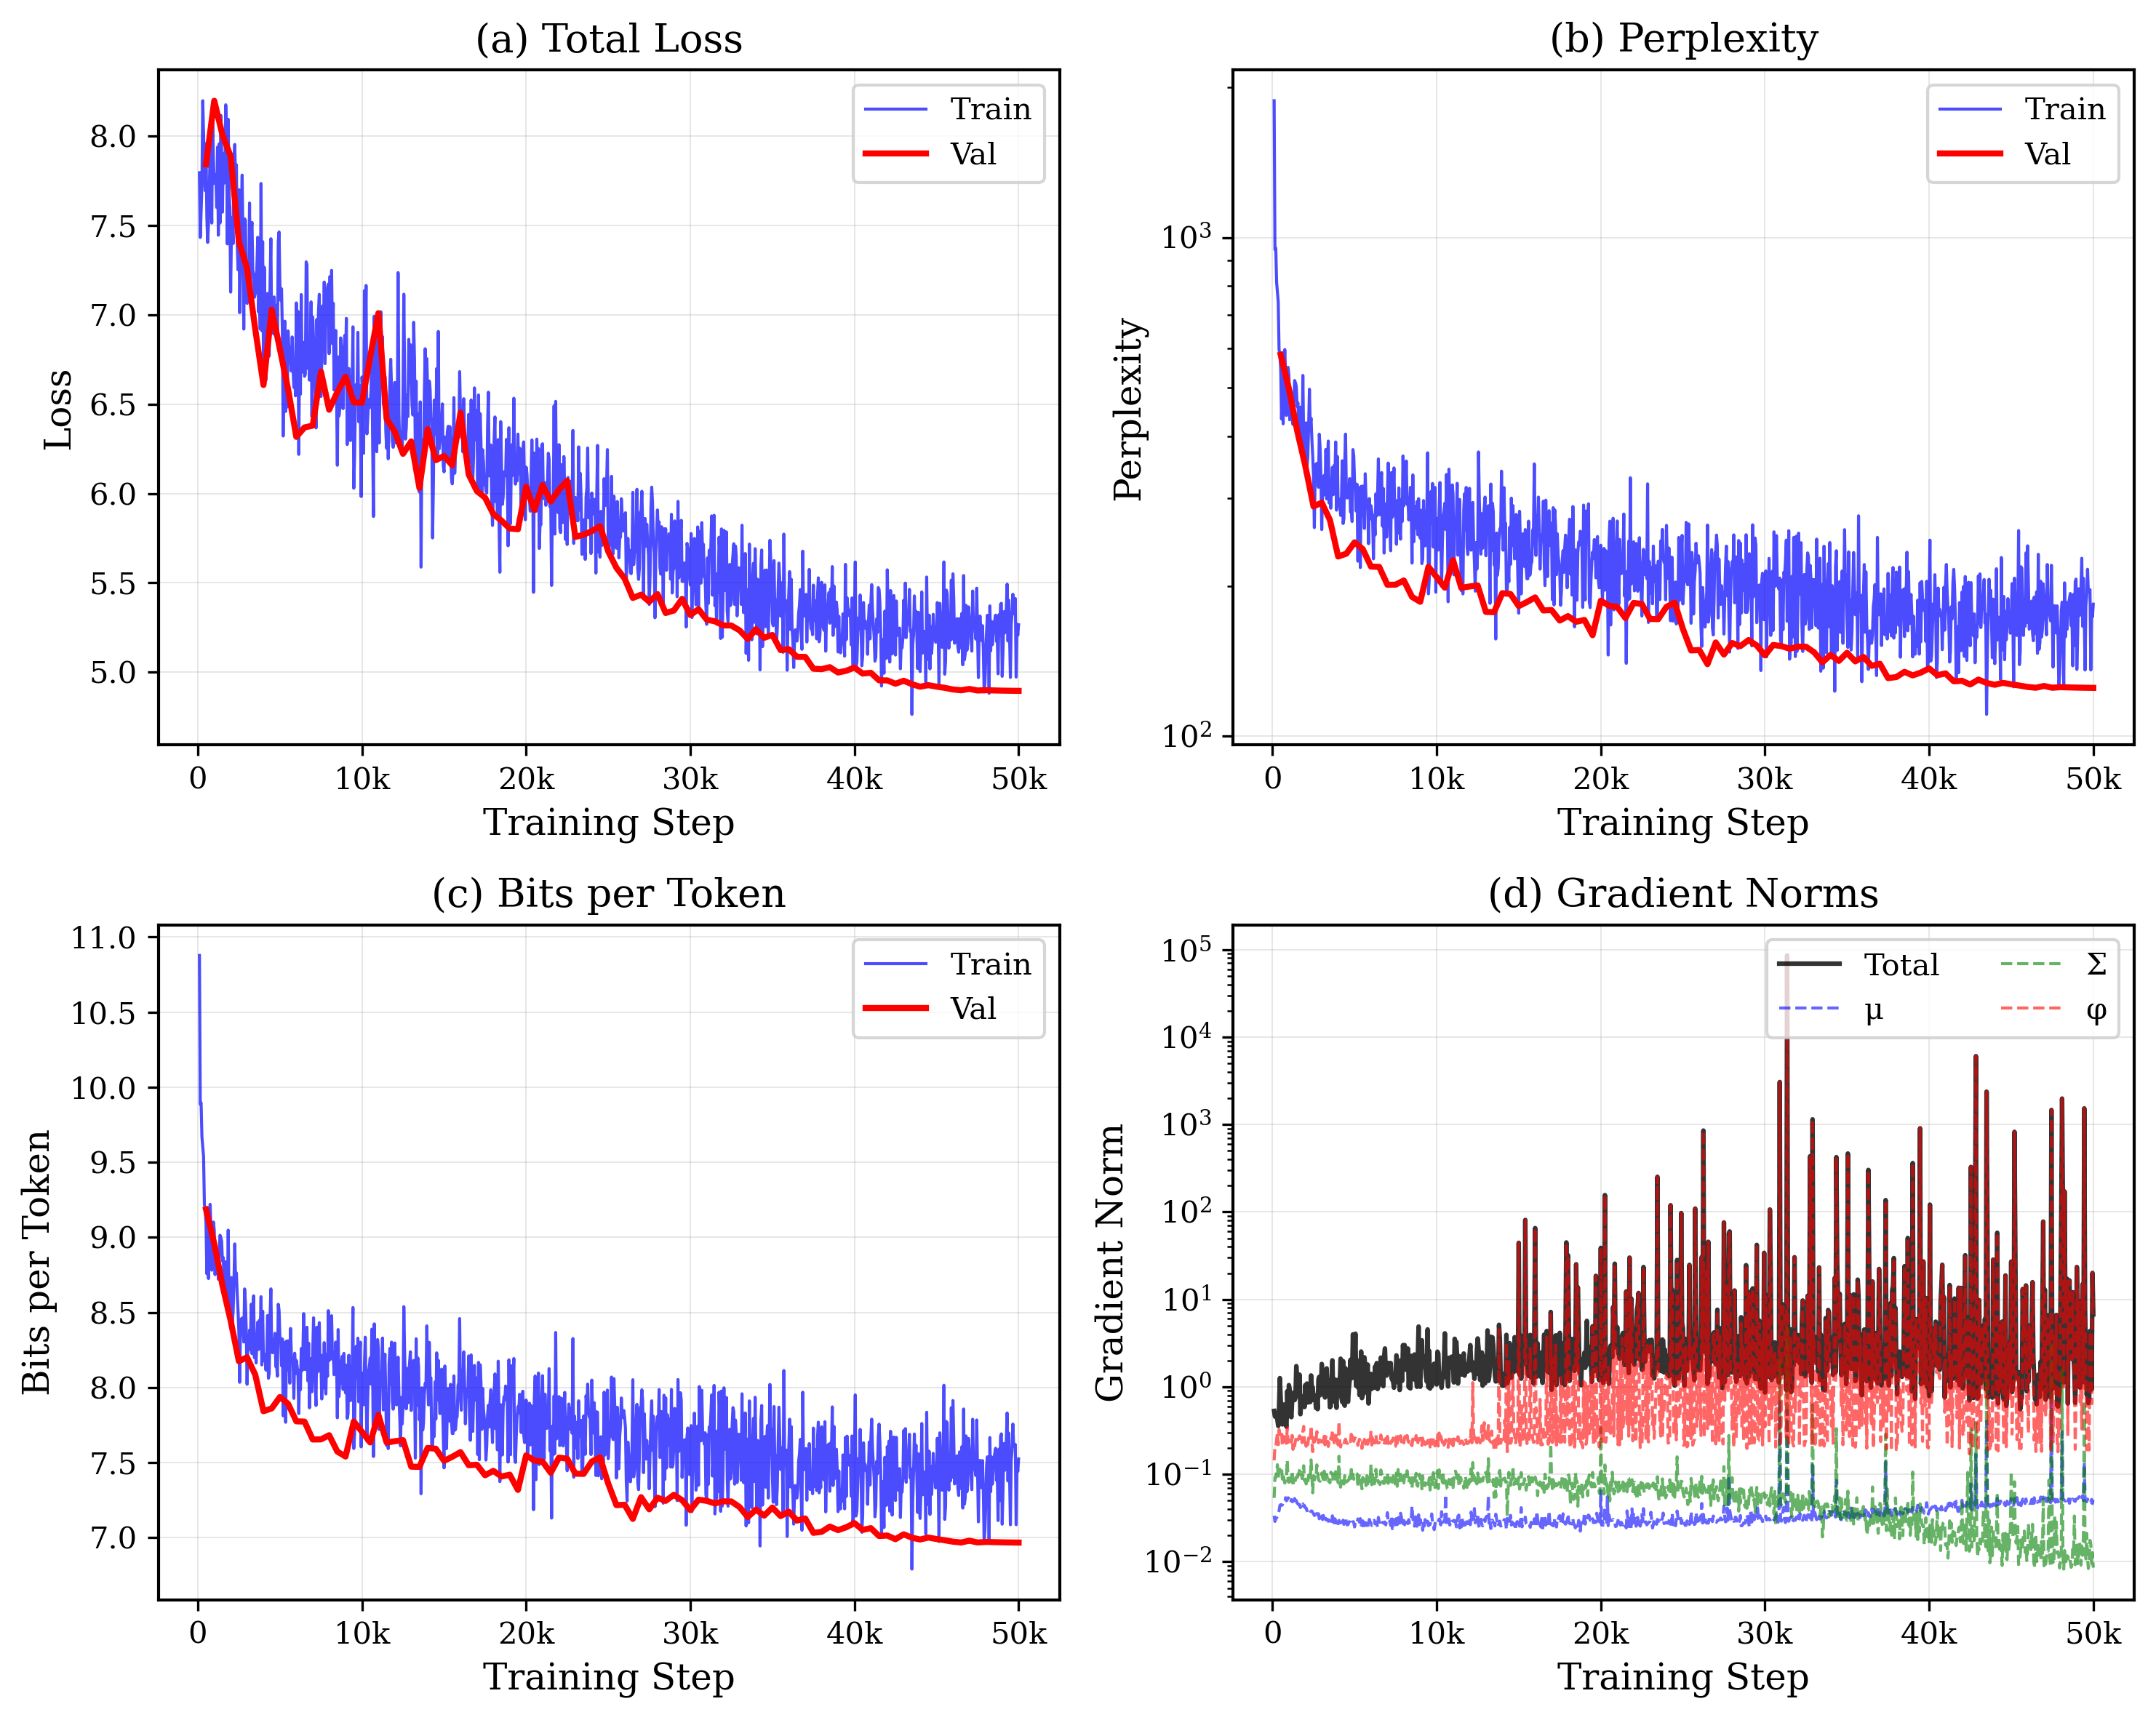
\includegraphics[width=\textwidth]{gl30_training_curves_3layer.png}
    \caption{3-layer $\mathrm{GL}(30)$ with trivial gauge transport}
  \end{subfigure}
  \hfill
  \begin{subfigure}[b]{0.48\textwidth}
    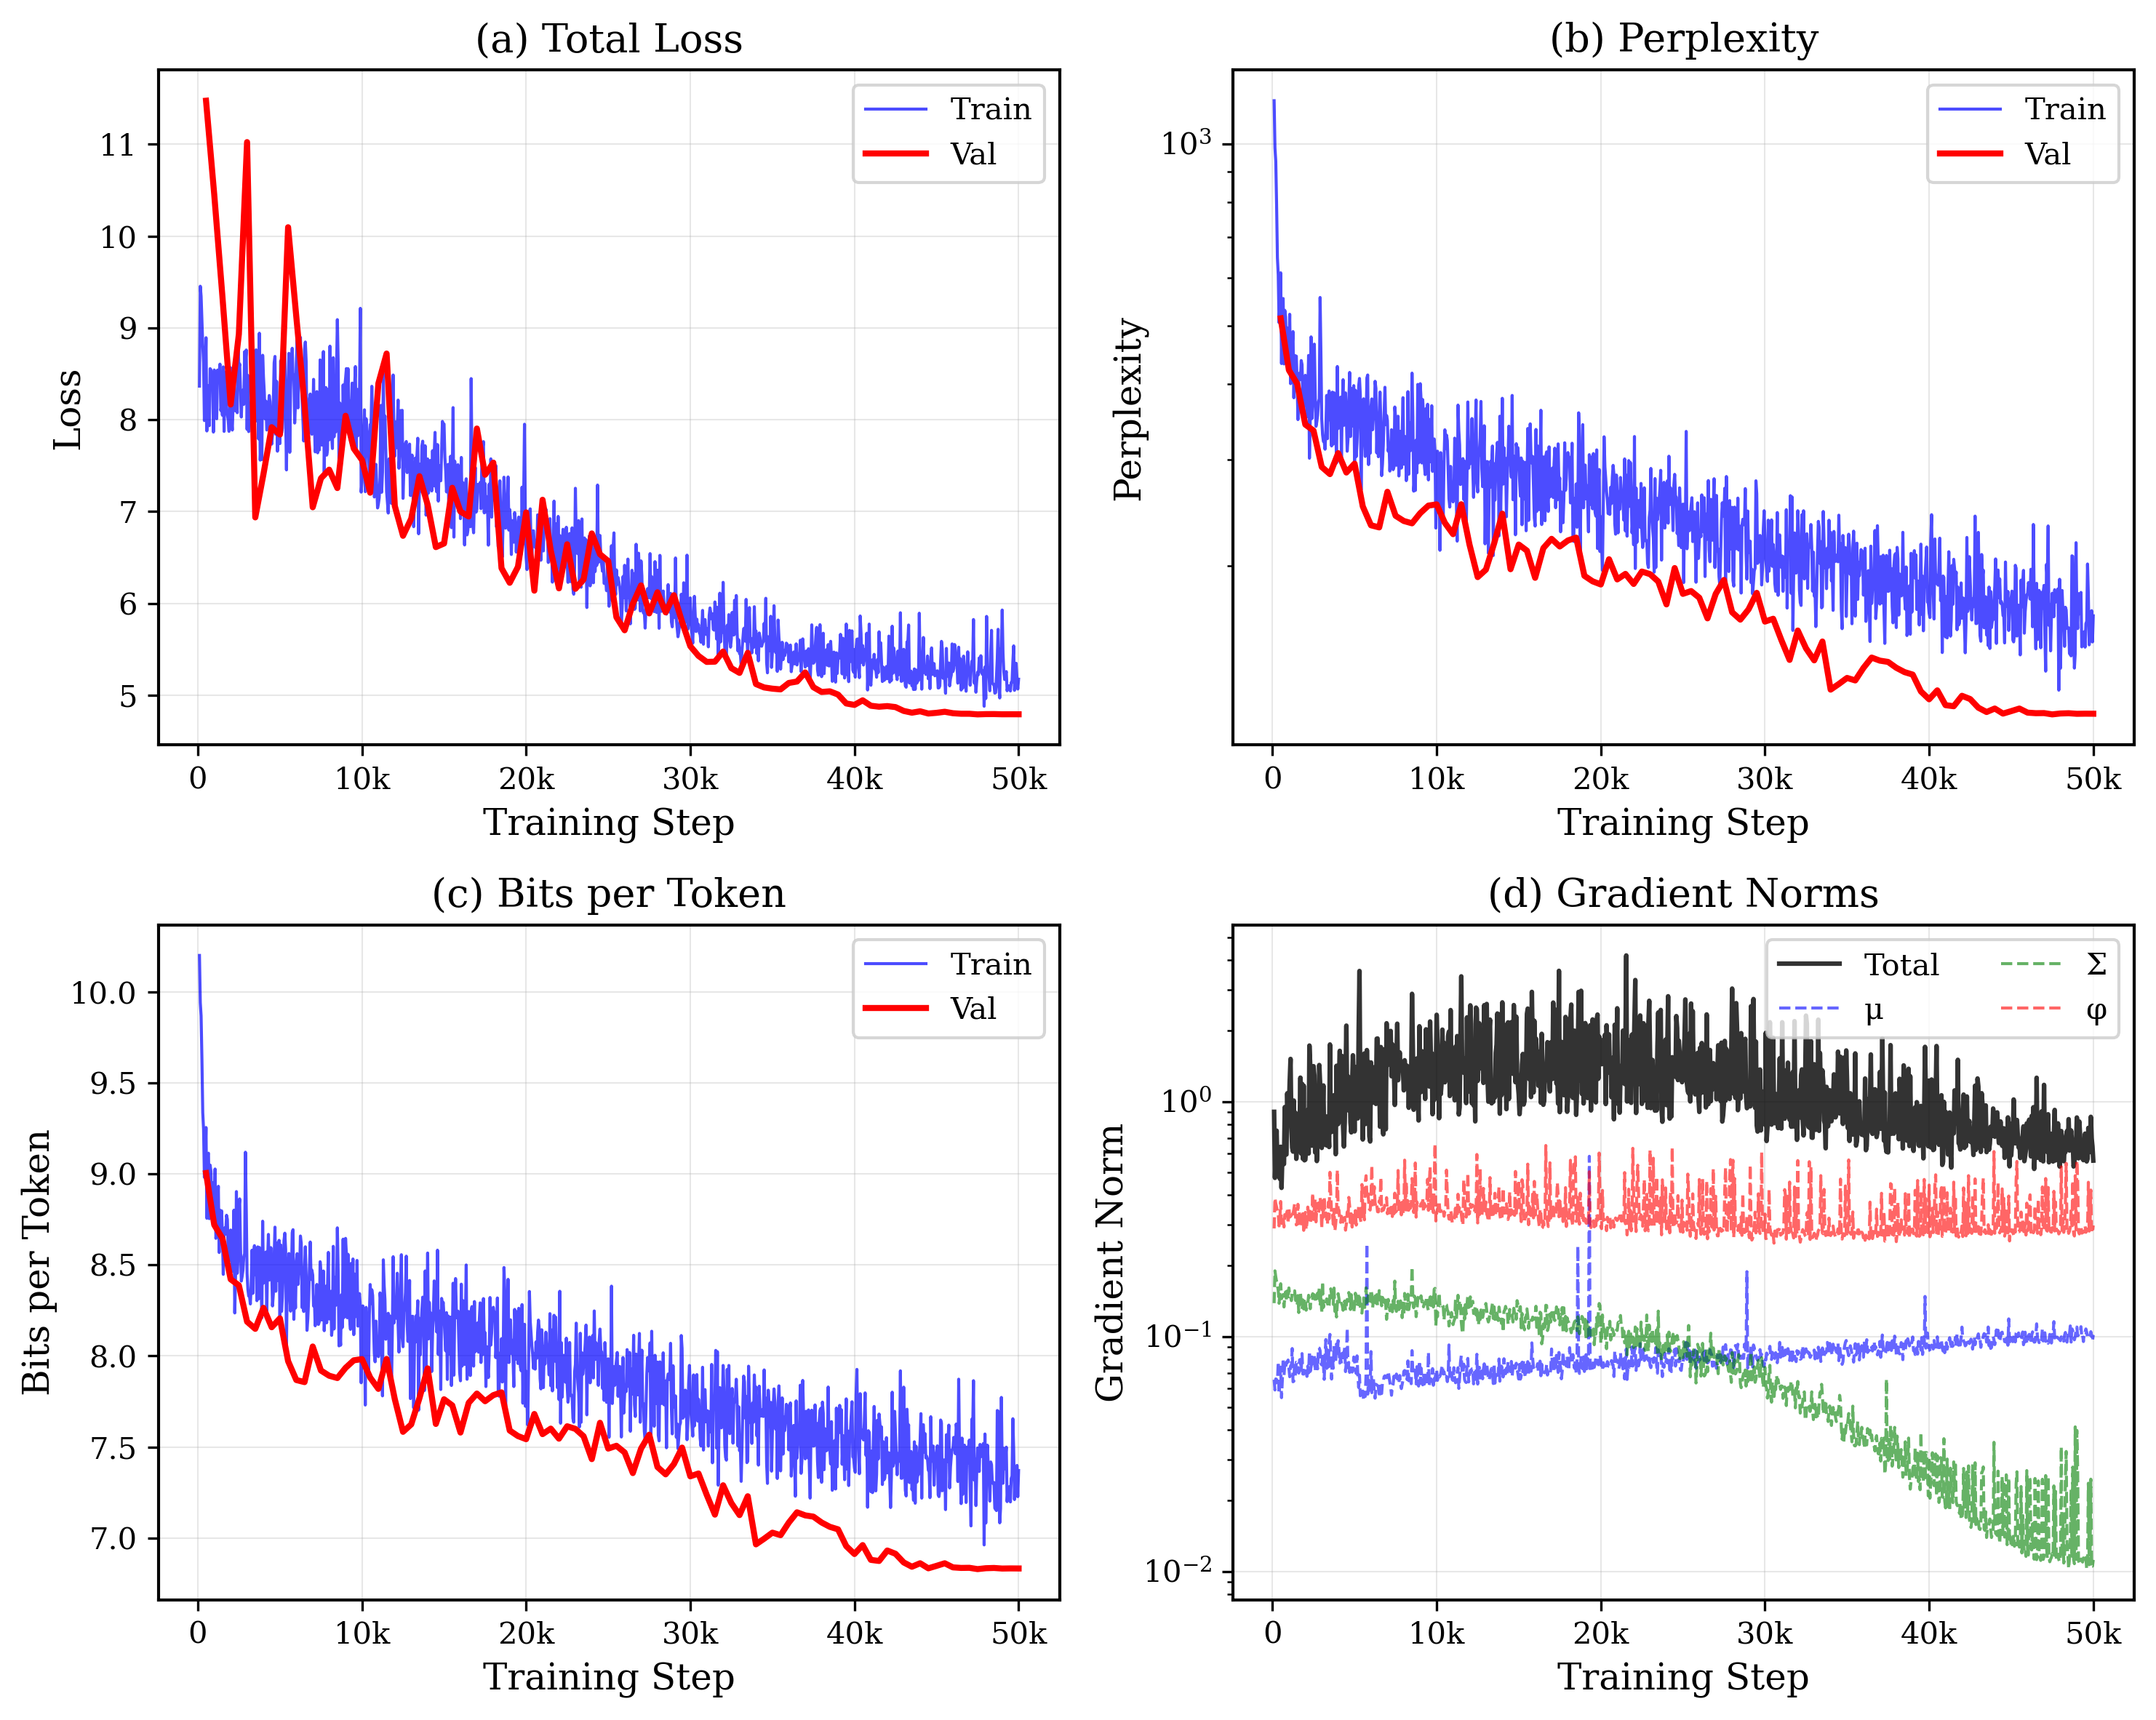
\includegraphics[width=\textwidth]{gl30_training_curves_1layer.png}
    \caption{1-layer $\mathrm{GL}(30)$ with learned gauge transport}
  \end{subfigure}
  \caption{Training dynamics for $\mathrm{GL}(30)$ gauge transformers on WikiText-103. (a,b) Total loss and perplexity vs.\ training step. (c) Bits per token. (d) Gradient norms decomposed by component: $\mu$ (beliefs), $\Sigma$ (covariances), $\phi$ (gauge frames). The 3-layer model converges faster (plateaus by step 25k) while the 1-layer learned-gauge model achieves better final perplexity (165 vs.\ 184) but requires longer training.}
  \label{fig:gl30_training}
\end{figure*}

\subsubsection{Comparison of Gauge Configurations}

The two configurations reveal a trade-off between architectural depth and gauge expressiveness:

\begin{table}[h]
\centering
\begin{tabular}{lcccc}
\hline
\textbf{Configuration} & \textbf{Layers} & \textbf{Gauge Mode} & \textbf{Train PPL} & \textbf{Test PPL} \\
\hline
Trivial gauge & 3 & Fixed $\Omega = I$ & 125.1 & 135.3 \\
Learned gauge & 1 & $\Omega \in \mathrm{GL}(30)$ & 113.9 & 151.8 \\
\hline
\end{tabular}
\caption{$\mathrm{GL}(30)$ language modeling results on WikiText-103.}
\label{tab:gl30_results}
\end{table}

The 3-layer trivial-gauge model generalizes better (lower test PPL) despite higher train PPL, suggesting the trivial gauge acts as an implicit regularizer. The 1-layer learned-gauge model achieves lower train perplexity, demonstrating that learning the full $\mathrm{GL}(K)$ gauge transformation provides additional expressiveness at the cost of some overfitting.

\subsubsection{Emergent Semantic Structure}

A striking finding is that both the learned belief embeddings $\mu$ and gauge frames $\phi$ develop interpretable semantic structure without explicit supervision. Figure~\ref{fig:gl30_semantic} shows PCA projections of the learned representations, with tokens colored by linguistic category (letter, digit, punctuation, function word, content word).

\begin{figure*}[t]
  \centering
  \begin{subfigure}[b]{0.48\textwidth}
    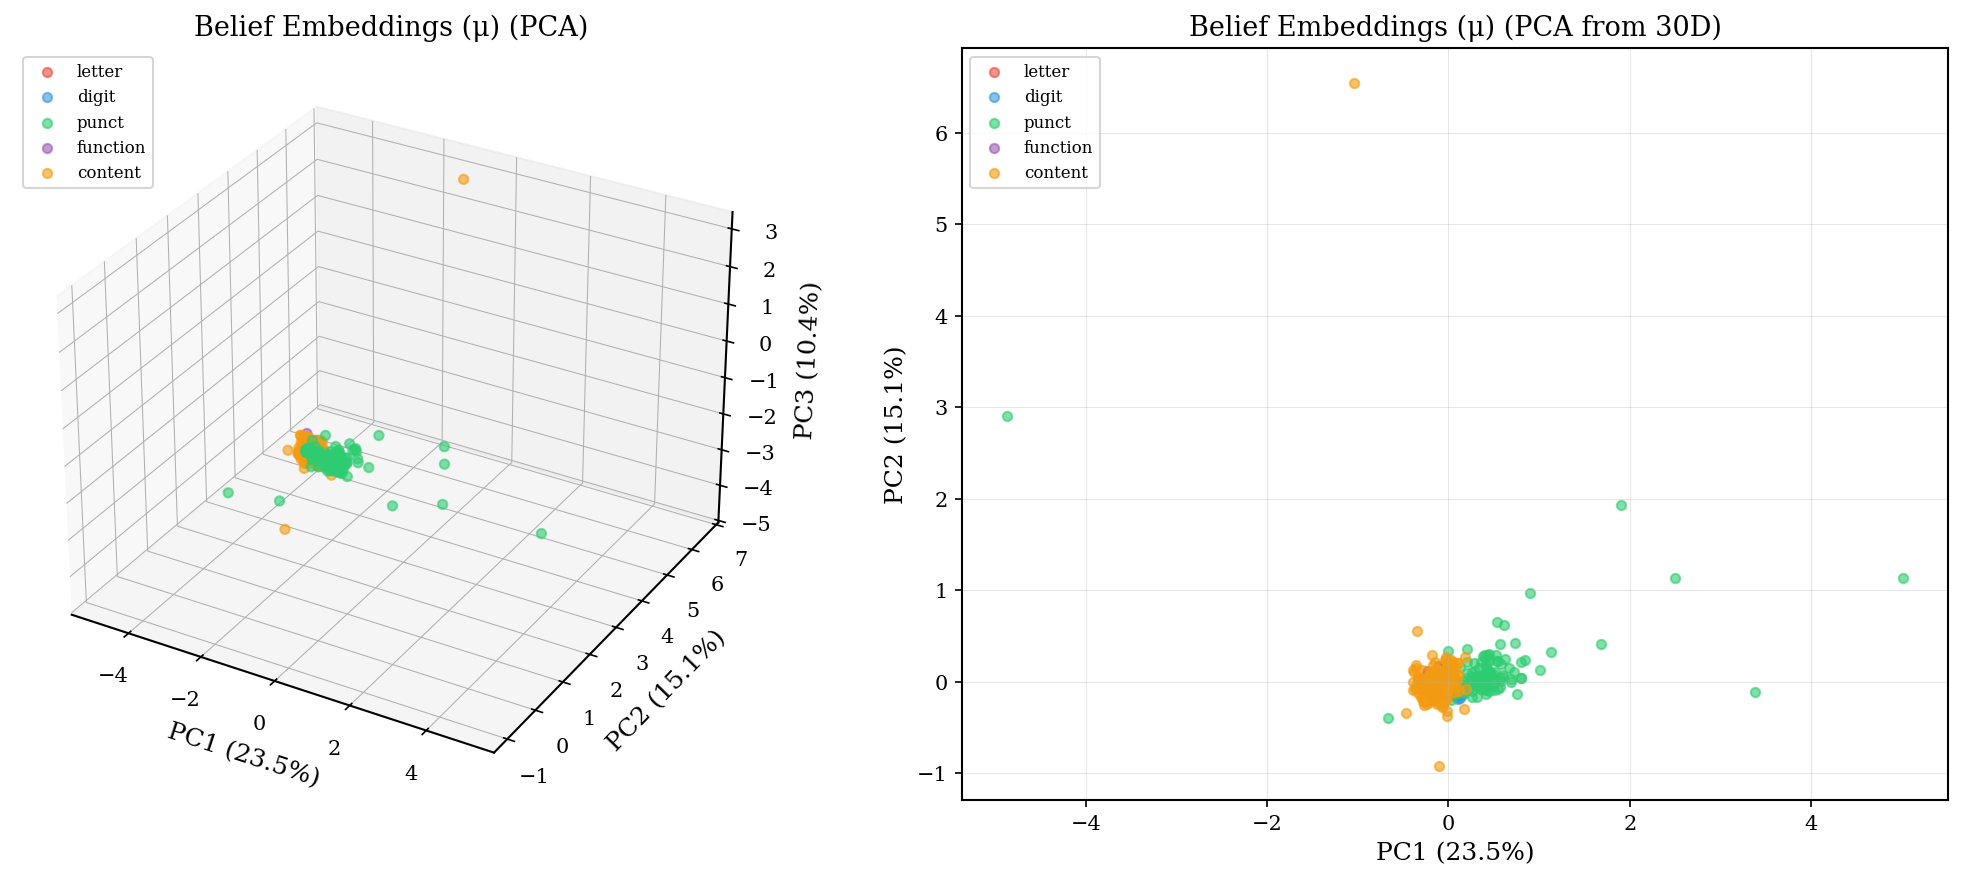
\includegraphics[width=\textwidth]{gl30_belief_clustering.png}
    \caption{Belief embeddings $\mu \in \mathbb{R}^{30}$}
  \end{subfigure}
  \hfill
  \begin{subfigure}[b]{0.48\textwidth}
    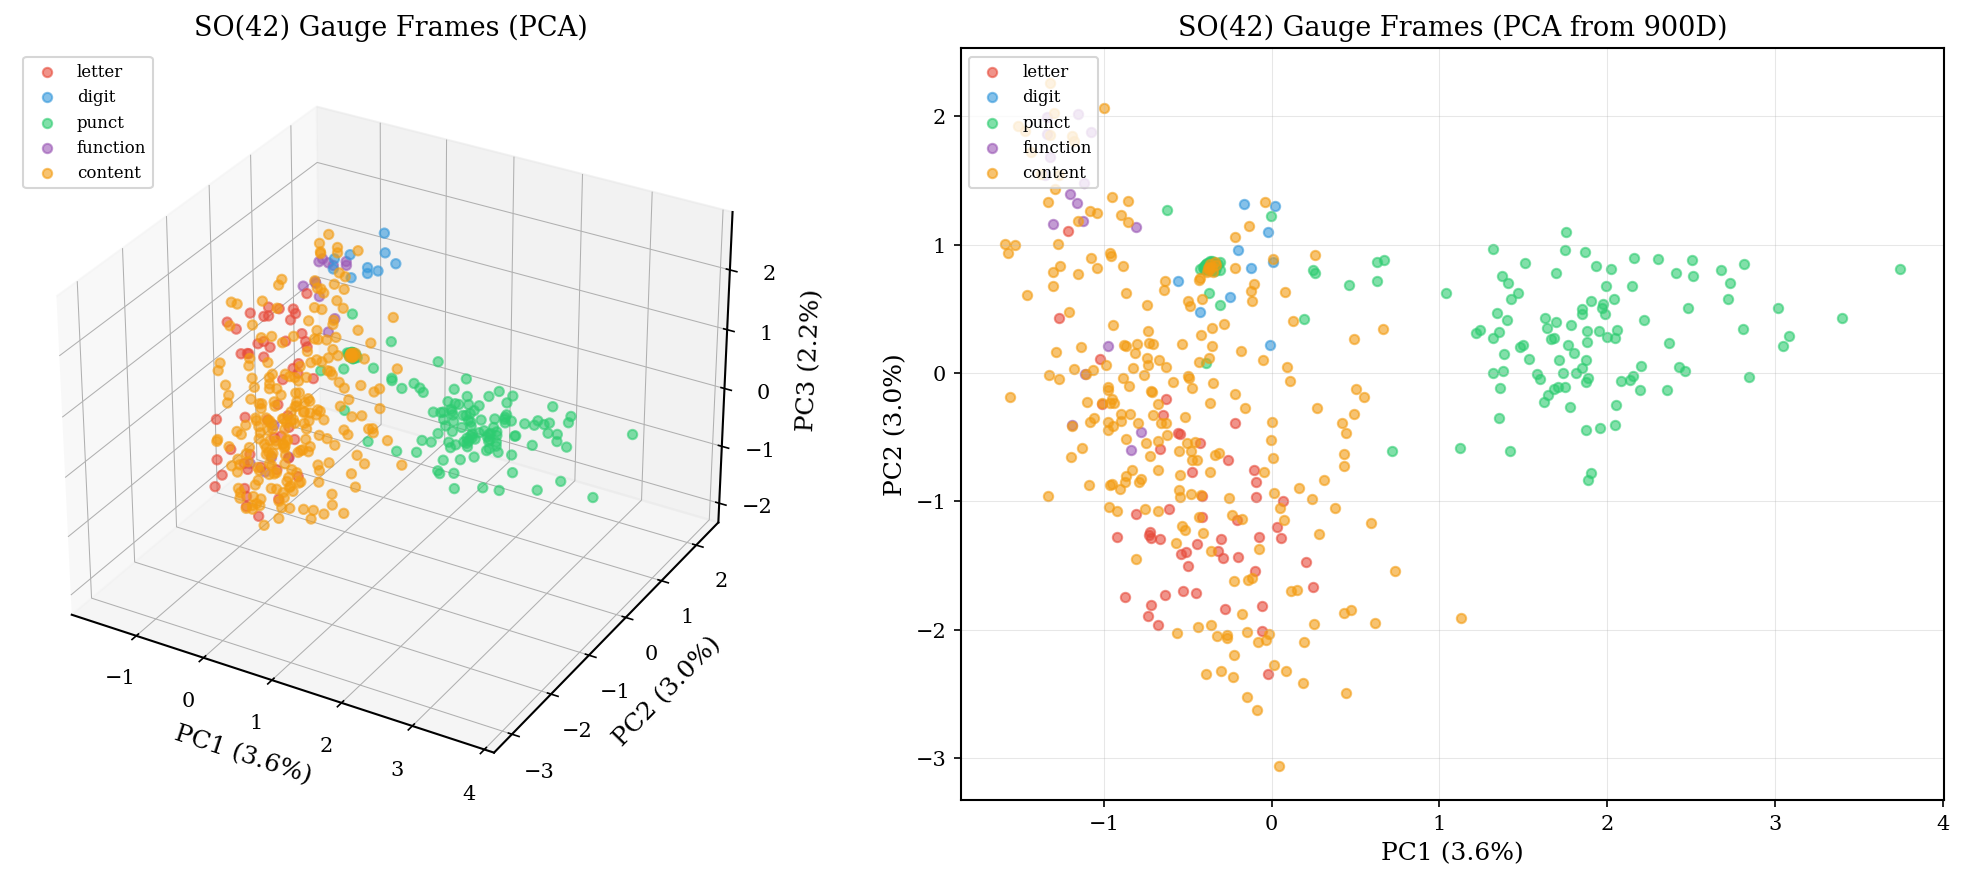
\includegraphics[width=\textwidth]{gl30_gauge_frame_clustering.png}
    \caption{Gauge frames $\phi \in \mathfrak{gl}(30) \cong \mathbb{R}^{900}$}
  \end{subfigure}
  \caption{Emergent semantic organization in learned $\mathrm{GL}(30)$ representations. \textbf{(a)} PCA of belief means $\mu$ shows punctuation tokens (green) spreading along principal components while content words (orange) and letters (red) form tighter clusters. \textbf{(b)} PCA of gauge frame coefficients $\phi$ reveals clear separation between linguistic categories: punctuation clusters distinctly from content words and letters. This structure emerges purely from the language modeling objective---no category labels are provided during training.}
  \label{fig:gl30_semantic}
\end{figure*}

\paragraph{Belief Embeddings.} The learned belief means $\mu \in \mathbb{R}^{30}$ show that punctuation tokens spread along the principal components while content words form a tighter central cluster. The first three principal components capture approximately 49\% of the variance, indicating moderate but interpretable low-dimensional structure.

\paragraph{Gauge Frames.} More remarkably, the gauge frame coefficients $\phi \in \mathfrak{gl}(30) \cong \mathbb{R}^{900}$ exhibit clear categorical separation. Punctuation tokens (green) cluster distinctly from content words (orange), with letters (red) forming a separate region. This organization emerges in a 900-dimensional space purely from the language modeling objective---the model was never told about linguistic categories.

This finding has important implications. The gauge frames $\phi$ parameterize the transport operators $\Omega = \exp(\phi)$ that mediate inter-token communication. The emergent categorical structure suggests that the model learns \emph{linguistically meaningful} transport---tokens of similar type communicate through similar geometric transformations. This provides evidence for the ``transport geometry over attention weighting'' hypothesis: the semantic content of attention is encoded not in which tokens attend to which, but in \emph{how} information is geometrically transformed during communication.

These results demonstrate that the gauge-theoretic framework scales to production language modeling tasks, with the theoretical constructs ($\mu$, $\Sigma$, $\phi$, KL-attention) functioning as intended during actual training.


\section{Discussion}

\subsection{Summary of Key Findings}

Our BERT validation (Section~5.2) demonstrated strong quantitative agreement between gauge-aligned and standard transformer attention across 144 heads (mean $r = 0.821$, median $r = 0.889$ at $\tau = 19.0$). While the overall correlation partly reflects the mathematical relationship between squared Euclidean distance and dot product under approximately constant norms, the framework generates non-trivial quantitative predictions that are confirmed: the optimal temperature $\tau = 19.0$ matches the prediction $\tau \approx 2\sqrt{d_k} = 16$ to within 19\%, and the key-norm bias ($\rho = -0.352$, significant in 92.4\% of heads) has both the predicted sign and magnitude.

\subsection{Language Modeling Without Neural Networks}

As detailed in Section~5.3, our $\mathrm{GL}(30)$ gauge VFE achieves test perplexity of 135 on WikiText-103 using \emph{zero} MLPs, activation functions, learned attention projections, or positional encodings. Only a linear output projection to vocabulary logits is retained. This result is intended as a proof of concept: the gauge-theoretic mathematical structure alone---KL divergences, transport operators, natural gradient descent---suffices for non-trivial language modeling. Controlled comparison against standard transformers of equal parameter count is needed to quantify the practical trade-offs and is left to future work. The depth vs.\ gauge expressiveness trade-off (Section~5.3.3) reveals that architectural depth and gauge expressiveness are partially substitutable.

A striking observation is that attention weights can converge to approximately uniform distributions while performance continues to improve, suggesting contextual information is encoded primarily in the transport operators $\Omega_{ij}$ rather than in selective attention weights. This supports the view that the essential computational structure of transformers lies in information-geometric relationships between token representations, not in the particular parameterization used to implement them.

\subsection{Architectural Insights}

Our results provide a principled explanation for empirical design choices in transformers. Layer normalization emerges as a geometric necessity that implements the high-dimensional cancellation condition required for frame-independent inference (Section~4.2.1). The temperature scaling $1/\sqrt{d}$ is the natural normalization arising from dimensional concentration of measure.

The per-layer correlation structure suggests that deeper layers (8--11) exhibit higher correlations with our KL attention, consistent with observations that semantic representations become more structured in deeper transformer layers. Heads achieving near-perfect correlation ($r \approx 1.00$) suggest these patterns may be universal features of distributed inference systems.

\subsection{Limitations and Future Directions}

Our validation tested the flat bundle limit where all frames are globally aligned and the connection is trivial. This is appropriate for comparison with standard transformers, which lack explicit gauge structure. However, the full power of the geometric framework lies in handling non-trivial bundles with curvature. Future work should explore whether introducing learned gauge transformations $\Omega_{ij}(c)$ can improve upon standard attention in certain tasks.

Our current comparison focused on the scaled isotropic limit where uncertainty covariances $\Sigma_i = \sigma^2 I$ are absorbed into learned projections. The full gauge theory incorporates non-trivial covariance matrices $\Sigma_i(c)$ that encode uncertainty about agent beliefs, corresponding to "fuzzy" vector embeddings in unique token/agent frames. Testing this framework against transformers with explicit uncertainty estimation (e.g., Bayesian neural networks, ensemble methods) represents an important future direction.

In Section 4.9, we developed the interpretation of multi-head attention as implementing irreducible representations of the gauge group. However, standard transformers use uniform head dimensions ($d_{\text{head}} = d/H$) rather than the geometrically natural dimensions dictated by irrep structure (e.g., $2\ell + 1$ for SO(3) irreps $\ell$). An intriguing question is whether transformers with non-uniform head dimensions matching irrep sizes could achieve better performance or sample efficiency on tasks with known symmetries.

While layer normalization mitigates key-norm bias uniformly across all tokens, the gauge-theoretic perspective suggests alternative strategies: rather than enforcing strict norm equality, one could learn optimal token norm profiles that trade off representational capacity (large norms encode more information) against attention quality (low norms avoid bias) in a Shannon-like manner. This could be implemented via soft norm constraints or adaptive normalization schedules that vary across layers or heads.

The geometric framework necessarily demands higher computational resources; however, sparse networks and other methods may enable training over reasonable time frames. The framework is not intended to offer economical benefits to deep learning, but rather to help researchers understand how and why these architectures perform as well as they do.

\subsection{Broader Implications}

Our results demonstrate that attention mechanisms can be understood as consequences of variational free energy minimization in gauge geometry: standard dot-product attention is recovered as a specific limit of a richer geometric framework. This perspective has conceptual value: it provides a mathematical interpretation of why attention works, predicts specific limitations (key-norm bias), and suggests principled extensions (gauge structure, uncertainty propagation). Machine learning can thus be interpreted as a symmetry-breaking phenomenon within a wider field theory.

By leveraging gauge theory coupled with informational geometry, we introduce geometric features that constrain model behavior according to standard symmetry principles---analogous to how convolutional neural networks impose translation equivariance or graph neural networks respect permutation invariance \citep{finzi2020generalizing,weiler20183d,kondor2018generalization}. The $\mathrm{GL}(K)$ invariance theorem reveals that standard transformers already implement the maximal gauge symmetry compatible with KL-based attention. Our framework shifts this paradigm toward a richer landscape where specific subgroups ($\mathrm{SO}(N)$, $\mathrm{SU}(N)$, Lorentz group) can be imposed as inductive biases, potentially enabling transformers to learn from fewer examples in domains with known physical structure or to infer patterns that unconstrained $\mathrm{GL}(K)$ would otherwise miss.

Standard attention transformers can be described as a 0-dimensional gauge theory in which all geometric structure is absorbed into learned parameters. This suggests a potentially powerful construction: $N$-dimensional fields of transformers coupled by induced gauge fields. The richness of differential geometry and information theory allows multiple lines of pursuit.

Most importantly, our work shows that attention can be understood as a consequence of agents minimizing a well-defined local variational free energy. The gauge-equivariant attention mechanism arises as an information aggregation strategy within this framework. Whether attention is a universal feature of multi-agent inference systems under geometric constraints---with implications beyond artificial neural networks to biological cognition and collective intelligence---remains a speculative but intriguing hypothesis that our framework makes mathematically precise and empirically testable.


\section{Conclusion}

We have shown that attention and transformer architecture emerge as limiting cases of a more general statistical gauge-equivariant theory where tokens are modeled as agents with beliefs that naturally descend a free energy functional. The attention dot-product emerges from an agent-agent ``communication'' term in a generalized variational energy functional as an application of the free energy principle. Gradient descent on this free energy recovers the standard training update, providing a variational interpretation of backpropagation in which each gradient term corresponds to an identifiable information-theoretic quantity.

The central interpretive insight is the $\mathrm{GL}(K)$ gauge structure of transformers: the learned projection matrices $W_Q, W_K$ are themselves gauge transformations with $\Omega = W_Q W_K^\top$ serving as a learned gauge transport (Theorem~\ref{thm:glk_invariance}). Standard transformers thus already implement gauge-theoretic attention with gauge structure absorbed into learned parameters. This explains why transformers can learn arbitrary (invertible) attention patterns: the $\mathrm{GL}(K)$ invariance of KL divergence guarantees that any invertible projection preserves the variational structure.

Our $\mathrm{GL}(30)$ language modeling experiments demonstrate that gauge-theoretic transformers---without MLPs, activation functions, or learned attention projections---achieve non-trivial language modeling (test perplexity $\sim$135 on WikiText-103) with emergent semantic structure in both belief and transport spaces. While not yet competitive with standard transformers of comparable size, these results validate that the gauge-theoretic mathematical structure alone carries meaningful computational content.

The framework exhibits a gauge-symmetric vacuum state (mirroring an untrained network) that undergoes spontaneous symmetry breaking under observations, providing a geometric interpretation of learning. We anticipate this perspective will find application not only in machine learning but also in understanding biological cognition, collective intelligence, and general informational systems where distributed agents must communicate under geometric constraints.





\section*{Acknowledgments}
Claude Sonnet 4.5 was utilized for programming our variational free energy descent simulation suite.  All code was manually reviewed, corrected, and mathematically validated by the author.  Furthermore, Claude was utilized for typesetting figures, LaTeX equations, and general organizational and manuscript clarity advice.  The author emphasizes that Claude (or any other LLMs) played no role in the development or conceptual ideas of our theoretical framework. The author further declares no funding or conflicts of interest.

\appendix



\subsection{General Mathematical Framework}
\subsubsection{Principal Bundle and Associated Bundles}

The following geometric and probabilistic constructions comprise standard methods in differential geometry and gauge theory.  See references for details, proofs, and examples \citep{nakahara2003geometry,frankel2011geometry,blei2017variational,amari2016information}.

Let $\pi: \mathcal{N} \to \mathcal{C}$ be a smooth principal $G$-bundle where $\mathcal{C}$ is a smooth manifold (the base space) and $G$ is a Lie group (the structure group) acting freely and transitively on the right on $\mathcal{N}$. The projection satisfies $\pi(n \cdot g) = \pi(n)$ for all $g \in G$, $n \in \mathcal{N}$.

Let $\rho_q: G \to \text{Aut}(\mathcal{B}_q)$ and $\rho_p: G \to \text{Aut}(\mathcal{B}_p)$ be representations of $G$ on smooth statistical manifolds $\mathcal{B}_q$ (belief/recognition fiber) and $\mathcal{B}_p$ (model/prior fiber). These fibers are typically:

\begin{itemize}
  \item $K$-dimensional probability simplices $\Delta^K$ (for categorical distributions), or
  \item Statistical manifolds with information-geometric structure (e.g., Gaussian manifolds, exponential families)
\end{itemize}

The associated bundles are:\\
\begin{align}
\mathcal{E}_q &:= \mathcal{N} \times_{\rho_q} \mathcal{B}_q = \left(\mathcal{N} \times \mathcal{B}_q\right)/\sim_q, \\
\mathcal{E}_p &:= \mathcal{N} \times_{\rho_p} \mathcal{B}_p = \left(\mathcal{N} \times \mathcal{B}_p\right)/\sim_p,
\end{align}\\
where $(n \cdot g, b) \sim_u (n, \rho_u(g)b)$ for $u \in \{q,p\}$.

These give fiber bundles $\pi_{\mathcal{E}_q}: \mathcal{E}_q \to \mathcal{C}$ and $\pi_{\mathcal{E}_p}: \mathcal{E}_p \to \mathcal{C}$ with fibers $\mathcal{B}_q(c) \cong \mathcal{B}_q$ and $\mathcal{B}_p(c) \cong \mathcal{B}_p$ at each $c \in \mathcal{C}$.

\subsection{Agents and Multi-Agent Systems}
Agent\\
An agent $\mathcal{A}^i$ is a pair of local sections over a domain $\mathcal{U}_i \subset \mathcal{C}$:

\begin{equation}
\mathcal{A}^i = \left(\sigma^i_q, \sigma^i_p\right),
\end{equation}

where $\sigma^i_q : \mathcal{U}_i \to \mathcal{E}_q$ and $\sigma^i_p : \mathcal{U}_i \to \mathcal{E}_p$.

We write $q_i(c) := \sigma^i_q(c) \in \mathcal{B}_q(c)$ and $p_i(c) := \sigma^i_p(c) \in \mathcal{B}_p(c)$ for the belief and model at base point $c$.

Multi-Agent System\\
A multi-agent system $\mathcal{M}$ over $\mathcal{C}$ is a collection of agents indexed by $\mathcal{I}$:

\begin{equation}
\mathcal{M} = \left\{\mathcal{A}^i = \left(\sigma^i_q, \sigma^i_p\right)\right\}_{i \in \mathcal{I}}.
\end{equation}

Agents generally overlap on intersections $\mathcal{U}_i \cap \mathcal{U}_j$.

Meta-Agent and Epistemic Death\\
A meta-agent is a multi-agent system whose component agents share identical section values on their overlap:

\begin{equation}
q_i(c) = q_j(c), \quad p_i(c) = p_j(c) \quad \text{for } c \in \mathcal{U}_i \cap \mathcal{U}_j.
\end{equation}

A set of agents is \emph{epistemically dead} if they identically share both beliefs and models. While constituent agents of a meta-agent may be epistemically dead, the meta-agent itself need not be; such agents can be integrated out, yielding coarse-grained higher-order entities and a route toward emergence.

\subsubsection{Bundle Morphisms and Transport Operators}
Via standard horizontal lifting from the principal bundle $\mathcal{N}$ to the associated bundles, we obtain a hierarchy of morphisms and induced connections:

\textbf{Intra-bundle transport:}

\begin{itemize}
  \item $\Omega^{(q)}_{ij}: \Gamma(\mathcal{B}_q) \to \Gamma(\mathcal{B}_q)$ (belief-to-belief)
  \item $\Omega^{(p)}_{ij}: \Gamma(\mathcal{B}_p) \to \Gamma(\mathcal{B}_p)$ (model-to-model)
\end{itemize}

\textbf{Cross-scale transport:}

\begin{itemize}
  \item $\Lambda^{s}_{s'}: \Gamma^{s}(\mathcal{B}_q) \to \Gamma^{s'}(\mathcal{B}_q)$ (beliefs across scales)
  \item $\tilde{\Lambda}^{s}_{s'}: \Gamma^{s}(\mathcal{B}_p) \to \Gamma^{s'}(\mathcal{B}_p)$ (models across scales)
\end{itemize}

\textbf{Inter-bundle morphisms:}

\begin{itemize}
  \item $\Theta^i_j: \Gamma(\mathcal{B}_q) \to \Gamma(\mathcal{B}_p)$ (belief to model)
  \item $\tilde{\Theta}^i_j: \Gamma(\mathcal{B}_p) \to \Gamma(\mathcal{B}_q)$ (model to belief)
\end{itemize}

\textbf{Global bundle morphisms:}

\begin{itemize}
  \item $\Phi: \mathcal{E}_p \to \mathcal{E}_q$ (model bundle to belief bundle)
  \item $\tilde{\Phi}: \mathcal{E}_q \to \mathcal{E}_p$ (belief bundle to model bundle)
\end{itemize}

Here $\Gamma(\mathcal{B}_u)$ denotes the space of smooth sections over the base $\mathcal{C}$.

\subsubsection{Gauge Frames and Connections}
Each agent $i$ possesses a local gauge frame field:

\begin{equation}
\phi_i: \mathcal{U}_i \to \mathfrak{g} = \text{Lie}(G),
\end{equation}

which induces a local connection one-form:

\begin{equation}
A^{(i)}_\mu(c) = U_i^{-1}(c) \partial_\mu U_i(c),
\end{equation}

where $U_i(c) = \exp[\phi_i(c)] \in G$. The associated field strength (gauge curvature) is:

\begin{equation}
F^{(i)}_{\mu\nu}(c) = \partial_\mu A^{(i)}_\nu - \partial_\nu A^{(i)}_\mu + [A^{(i)}_\mu, A^{(i)}_\nu] \in \mathfrak{g}.
\end{equation}

When two agents overlap at $c \in \mathcal{U}_i \cap \mathcal{U}_j$, the inter-agent gauge transformation:

\begin{equation}
\Omega_{ij}(c) = \exp[\phi_i(c)] \exp[-\phi_j(c)] \in G
\end{equation}

transports agent $j$'s representations into agent $i$'s frame:

\begin{equation}
q_j(c) \mapsto \Omega_{ij}(c) \cdot q_j(c) := \rho(\Omega_{ij}(c)) q_j(c).
\end{equation}

On overlaps, local connections are related by:

\begin{equation}
A^{(i)}_\mu = \Omega_{ij} A^{(j)}_\mu \Omega_{ij}^{-1} + \Omega_{ij} \partial_\mu \Omega_{ij}^{-1}.
\end{equation}

\subsubsection{Curvature Structure}
The full framework incorporates four distinct types of curvature:

Statistical Manifold Curvature

The fiber $\mathcal{B}$ has intrinsic curvature tensor:

\begin{equation}
R^\mathcal{B}(X,Y)Z = \nabla_X \nabla_Y Z - \nabla_Y \nabla_X Z - \nabla_{[X,Y]} Z.
\end{equation}

This measures the geometry of the space of probability distributions (e.g., Gaussian manifolds have constant negative curvature).

Gauge Group Curvature.

The structure group $G$ itself is a curved manifold. For $G = SO(3)$:

\begin{itemize}
  \item Topology: $SO(3) \cong \mathbb{RP}^3$
  \item Constant positive sectional curvature
  \item Non-commutativity: $\Omega_{ij}\Omega_{jk} \neq \Omega_{jk}\Omega_{ij}$ in general
\end{itemize}

Gauge Field Curvature.\\
The connection $A_\mu$ has field strength $F_{\mu\nu}$ measuring path-dependence of parallel transport through the base space $\mathcal{C}$.

Base Manifold Curvature.

If $\mathcal{C}$ carries a Riemannian metric $g_{\mathcal{C}}$, its curvature tensor:

\begin{equation}
R^\mathcal{C}(X,Y)Z = \nabla^\mathcal{C}_X \nabla^\mathcal{C}_Y Z - \nabla^\mathcal{C}_Y \nabla^\mathcal{C}_X Z - \nabla^\mathcal{C}_{[X,Y]} Z
\end{equation}

affects the geometry of the latent space agents inhabit.






\section{Covariance Dynamics and Equilibrium Analysis}
\label{app:covariance_dynamics}

\subsection{Covariance Gradient of the Generalized Free Energy}

Here we derive the gradient of the single-agent free energy $\mathcal{F}_i$ with respect to the covariance $\Sigma_i$ for agent $i$; a well known result in information geometry.

The free energy decomposes as

\begin{equation}
\mathcal{F}_i
=D_{\mathrm{KL}}(q_i \,\|\, p_i)
+ \sum_{j \neq i} \beta_{ij}\,
D_{\mathrm{KL}}(q_i \,\|\, \Omega_{ij} q_j)
- \mathbb{E}_{q_i}[\log p(o_i \mid k_i)],
\end{equation}

where $q_i = \mathcal{N}(\mu_i, \Sigma_i)$, $p_i = \mathcal{N}(\mu_{p,i}, \Sigma_{p,i})$, and $\sum_j \beta_{ij} = 1$ by construction.

\subsubsection{Gaussian KL divergence and its derivative}

For two Multivariate Gaussians, we have 

\begin{align}
D_{\mathrm{KL}}\!\left(
\mathcal{N}(\mu_1, \Sigma_1)
\,\|\, 
\mathcal{N}(\mu_2, \Sigma_2)
\right)
&=
\frac{1}{2}
\Big[
\log \frac{|\Sigma_2|}{|\Sigma_1|}
+ \mathrm{tr}\!\big(\Sigma_2^{-1}\Sigma_1\big)
\\ &\quad
+ (\mu_2 - \mu_1)^\top
  \Sigma_2^{-1}
  (\mu_2 - \mu_1)
- d
\Big].
\label{eq:gaussian_KL}
\end{align}


and differentiating w.r.t.\ $\Sigma_1$ (holding $\mu_1,\mu_2,\Sigma_2$ fixed) gives

\begin{equation}
\frac{\partial D_{\mathrm{KL}}}{\partial \Sigma_1}
=\frac{1}{2}\left[
-\Sigma_1^{-1}
+ \Sigma_2^{-1}
\right].
\end{equation}

Applying this to each term in $\mathcal{F}_i$:

\begin{align}
\frac{\partial}{\partial \Sigma_i}
D_{\mathrm{KL}}(q_i \,\|\, p_i)
&=\frac{1}{2}\left[
-\Sigma_i^{-1}
+ \Sigma_{p,i}^{-1}
\right],
\\[6pt]
\frac{\partial}{\partial \Sigma_i}
D_{\mathrm{KL}}(q_i \,\|\, \Omega_{ij} q_j)
&=
\frac{1}{2}\left[
-\Sigma_i^{-1}
+ (\Omega_{ij}\Sigma_j\Omega_{ij}^\top)^{-1}
\right].
\end{align}

The observation term contributes an $O(\Sigma_i^{-1})$ correction that we neglect in the high-precision / strong-alignment regime. Thus

\begin{equation}
\boxed{
\frac{\partial \mathcal{F}_i}{\partial \Sigma_i}
=\frac{1}{2}
\left[
-2 \Sigma_i^{-1}
+ \Sigma_{p,i}^{-1}
+ \sum_j \beta_{ij}
(\Omega_{ij}\Sigma_j\Omega_{ij}^\top)^{-1}
\right].
}
\label{eq:Sigma_gradient_final}
\end{equation}

Because $\sum_j \beta_{ij} = 1$, there is no $(1 + \sum_j \beta_{ij})$ prefactor in front of $\Sigma_i^{-1}$.

\subsection{Fixed-Point Equation and Symmetric Solution}

At equilibrium, we set $\partial \mathcal{F}_i / \partial \Sigma_i = 0$, giving

\begin{equation}
\Sigma_i^{-1}
=\frac{1}{2}
\left[
\Sigma_{p,i}^{-1}
+ \sum_j \beta_{ij}
(\Omega_{ij}\Sigma_j\Omega_{ij}^\top)^{-1}
\right].
\label{eq:sigma_fixed_point_beta}
\end{equation}

This is a matrix-valued fixed-point equation coupling all agents: each agent’s precision is the $\beta$-weighted combination of its own prior precision and the transported neighbor precisions.

\subsubsection{Homogeneous limit}

In the homogenous limit we assume 

(i) all agents are identical, so $\Sigma_i = \Sigma_\infty$ for all $i$,

(ii) $\Omega_{ij} \approx I$ (weak misalignment),

(iii) $\Sigma_{p,i} = \Sigma_0$ (shared prior).

Then \eqref{eq:sigma_fixed_point_beta} becomes

\begin{equation}
\Sigma_\infty^{-1}
=\frac{1}{2}
\left[
\Sigma_0^{-1}
+ \Sigma_\infty^{-1}
\right]
\quad\Longrightarrow\quad
\Sigma_\infty = \Sigma_0.
\end{equation}

Hence, in a perfectly symmetric population, the equilibrium covariance reproduces the shared prior.

\subsubsection{Alignment-dominated regime}

Although $\sum_j \beta_{ij} = 1$, the effective strength of alignment is controlled by the parameter $\tau$ in

\begin{equation}
\beta_{ij}
=\frac{
\exp\!\left[
-\frac{1}{\tau}
D_{\mathrm{KL}}\!\big(q_i \,\|\, \Omega_{ij} q_j\big)
\right]
}{\sum_k
\exp\!\left[
-\frac{1}{\tau}
D_{\mathrm{KL}}\!\big(q_i \,\|\, \Omega_{ik} q_k\big)
\right]}.
\end{equation}

As $\tau \to 0$, $\beta_{ij}$ becomes sharply peaked on whichever neighbor $j$ best agrees (after transport). In that low-$\tau$ limit, the prior precision $\Sigma_{p,i}^{-1}$ becomes negligible relative to the socially enforced alignment term, and

\begin{equation}
\boxed{
\Sigma_i^{-1}
\;\approx\;
\sum_j \beta_{ij}
(\Omega_{ij}\Sigma_j\Omega_{ij}^\top)^{-1}
\;=\;\big\langle(\Omega_{ij}\Sigma_j\Omega_{ij}^\top)^{-1}
\big\rangle_{\beta}.}
\label{eq:beta_weighted_precision}
\end{equation}

Here $\langle \cdot \rangle_{\beta}$ denotes a $\beta$-weighted expectation over neighbors.  

Therefore, in the strong-alignment (i.e. small $\tau$) regime, agent $i$’s precision matrix becomes the $\beta$-weighted average of its neighbors' transported precisions.

When, additionally, all agents already have approximately equal covariances and the transports are near-identity, i.e. $\Sigma_i \approx \Sigma_j$ and $\Omega_{ij} \approx I$, then \eqref{eq:beta_weighted_precision} implies

\begin{equation}
\Sigma_i^{-1} \approx \Sigma_j^{-1}
\quad\Longrightarrow\quad
\Sigma_i \approx \Omega_{ij}\Sigma_j\Omega_{ij}^\top,
\end{equation}

justifying the alignment assumption used in the main text.

\subsubsection{Gradient flow dynamics}

Finally, consider the gradient flow

\begin{equation}
\frac{d\Sigma_i}{dt}
=-\eta_\Sigma
\frac{\partial \mathcal{F}_i}{\partial \Sigma_i},
\qquad\eta_\Sigma > 0.
\end{equation}

Local stability of the equilibrium \eqref{eq:sigma_fixed_point_beta} follows from the positive-definiteness of the Hessian. For the Gaussian KL terms,

\begin{equation}
\frac{\partial^2 D_{\mathrm{KL}}}{\partial \Sigma_1 \, \partial \Sigma_1}
\;\sim\;
\Sigma_1^{-1} \otimes \Sigma_1^{-1}
+ \Sigma_2^{-1} \otimes \Sigma_2^{-1},
\end{equation}

which is manifestly positive definite for $\Sigma_1,\Sigma_2 \succ 0$.

Hence the covariance alignment fixed-point is an attractor of the variational dynamics.

Therefore, we find that $\Sigma_i \approx \Omega_{ij}\Sigma_j\Omega_{ij}^\top$ emerges from the dynamics itself rather than as an imposed constraint.
















\section{Conditional Uniqueness of the Forward KL Divergence via Variational Duality}

We now show that, within a broad but well-defined class of variational games, the forward KL divergence $D_{\mathrm{KL}}(q_i \,\|\, \Omega_{ij} q_j)$ is the only divergence that yields a closed-form Gibbs-type solution for the belief update and a consistent dual interpretation for the attention weights.  Agents locally minimize their agent-specific variational free energy and the system of agents minimize their collective global free energies.  This local-global coordination gives rise to the expected forward KL attention term.

Here we are restricting the the matched-fiber case.  The full generalization follows by applying the appropriate bundle morphisms/intertwiners.

The uniqueness of this term is conditional and follows from three assumptions:

\begin{enumerate}
  \item $\mathcal{D}$ is local in $c$, of f-divergence form $\displaystyle \int q_i(c)\, f\!\left(\frac{q_i(c)}{\Omega_{ij}(c) q_j(c)}\right) dc$,
  \item the coupling is linear
  \item the minimizing belief, $q_i^*$, remains in the exponential-family (log-linear) class.
\end{enumerate}

\subsubsection{The Coupled Variational Problem}
Each agent $i$ minimizes a local free-energy functional:

\begin{equation}
F_i[\beta_i]
=\min_{q_i}
\Big\{
D_{\mathrm{KL}}(q_i \,\|\, p_i)
+ \sum_{j\neq i} \beta_{ij}\,\mathcal{D}(q_i,q_j)
\Big\},
\label{eq:F_i}
\end{equation}

For notational convenience, we can decompose the KL divergence as:

\begin{equation}
D_{\mathrm{KL}}(q_i \,\|\, p_i) = \langle H_i \rangle_{q_i} + S(q_i) + \text{const},
\end{equation}

where

\begin{align}
H_i(c) &:= -\log p_i(c) \quad \text{(local "energy")}, \\
S(q_i) &:= -\int q_i(c) \log q_i(c)\,dc \quad \text{(Shannon entropy)}, \\
\langle H_i \rangle_{q_i} &:= \int q_i(c) H_i(c)\,dc \quad \text{(expected energy)}.
\end{align}

This gives $D_{\mathrm{KL}}(q_i \,\|\, p_i) = \int q_i(c)[\log q_i(c) - \log p_i(c)]\,dc$.

The attention weights $\beta_{ij}\ge 0$ (with $\sum_j \beta_{ij}=1$) are subsequently chosen by optimizing

\begin{equation}
\mathcal{J}_i(\beta_i)
=\sum_{j\neq i}\beta_{ij} C_{ij}
+ \tau \sum_{j\neq i}\beta_{ij}\log\beta_{ij},
\label{eq:J_i}
\end{equation}

where $C_{ij}$ denotes the marginal cost of attending to agent $j$ as we've described above.

We shall later identify

\begin{equation}
C_{ij} := \frac{\partial S_i}{\partial \beta_{ij}},
\end{equation}

so that attention weights allocate resources in proportion to marginal coordination penalties.

\subsubsection{Forward KL and the Geometric-Mean Solution}
Let $\mathcal{D}(q_i,q_j) = D_{\mathrm{KL}}(q_i \,\|\, \Omega_{ij} q_j)$, where

\[
\frac{\delta D_{\mathrm{KL}}(q_i \,\|\, \Omega_{ij} q_j)}{\delta q_i(c)} 
= \log\frac{q_i(c)}{\Omega_{ij}(c) q_j(c)} + 1.
\]

The stationary condition for \eqref{eq:F_i} is

\begin{equation}
H_i(c)
+ \log q_i(c)
+ \sum_j \beta_{ij}
\!\left[
\log\frac{q_i(c)}{\Omega_{ij}(c)q_j(c)}+1
\right]
= \lambda_i,
\end{equation}

with $\lambda_i$ enforcing normalization.

Rearranging and solving for $q_i(c)$ gives a Boltzmann distribution whose mean field is a geometric average of transported neighbor beliefs.

\begin{equation}
q_i^*(c)
= \frac{1}{Z_i}
e^{-H_i(c)/2}
\prod_j
[\Omega_{ij}(c) q_j(c)]^{\beta_{ij}/2},
\label{eq:q_i_star}
\end{equation}

This structure is preserved only for the forward KL divergence; alternative divergences destroy the log-linearity of the exponent.

\subsubsection{Dual Relation via the Envelope Theorem}
At the stationary value $q_i^*$, the envelope theorem implies

\begin{equation}
\frac{\partial F_i}{\partial \beta_{ij}}
= \mathcal{D}(q_i^*, q_j)
= D_{\mathrm{KL}}(q_i^* \,\|\, \Omega_{ij} q_j),
\label{eq:envelope}
\end{equation}

such that the marginal cost of increasing attention to $j$ equals the forward KL divergence between the updated belief $q_i^*$ and the transported neighbor $\Omega_{ij} q_j$ into $i$'s frame.

This identifies the attention cost with the KL.

\subsubsection{Reverse and Symmetric KL Forms}
If instead $\mathcal{D}(q_i,q_j) = D_{\mathrm{KL}}(\Omega_{ij}q_j \,\|\, q_i)$, the stationary condition becomes

\begin{equation}
H_i(c)
+ \log q_i(c)
- \sum_j \beta_{ij}
\frac{\Omega_{ij}(c) q_j(c)}{q_i(c)}
= \text{const},
\end{equation}

introducing terms as $1/q_i$ and leading to a transcendental stationary equation without a closed-form solution destroying the exponential family requirement above.

Likewise, the symmetrized divergence

\[
\mathcal{D}_{\mathrm{sym}}(q_i,q_j)
= \tfrac{1}{2}\!\left[
D_{\mathrm{KL}}(q_i \,\|\, \Omega_{ij} q_j)
+ D_{\mathrm{KL}}(\Omega_{ij} q_j \,\|\, q_i)
\right]
\]

mixes $\log q_i$ and $1/q_i$ terms, again breaking log-linearity.\\
Hence, among local f-divergences, only the forward KL preserves exponential-family closure.

\subsubsection{Conditional Uniqueness Theorem}
Let $\mathcal{D}(q_i,q_j)$ be any local $f$-divergence

\[
\mathcal{D}(q_i,q_j)
= \int q_i(c)\,
f\!\left(\frac{q_i(c)}{\Omega_{ij}(c) q_j(c)}\right)
dc,
\]

that enters linearly in \eqref{eq:F_i}, and further suppose that the stationary distribution $q_i^*$ is log-linear in $\{H_i,\Omega_{ij}q_j\}$.

Then the following are equivalent:

\begin{enumerate}
  \item $q_i^*$ has the geometric-mean Boltzmann form \eqref{eq:q_i_star};
  \item $\mathcal{D}(q_i,q_j)=D_{\mathrm{KL}}(q_i \,\|\, \Omega_{ij} q_j)$;
  \item $C_{ij}=\dfrac{\partial F_i}{\partial\beta_{ij}}
=D_{\mathrm{KL}}(q_i^* \,\|\, \Omega_{ij}q_j).$
\end{enumerate}

Proof sketch

(2) $\Rightarrow$ (1) follows from direct solution of the stationary condition.

(1) $\Rightarrow$ (2):

Assume the solution is log-linear \eqref{eq:q_i_star}.\\
Substituting this into the stationarity condition gives

\[
\frac{\delta \mathcal{D}}{\delta q_i(c)}
\Big|_{q_i^*}
= \log\frac{q_i^*(c)}{\Omega_{ij}(c) q_j(c)} + 1.
\]

Next, integrating, we find

\[
\mathcal{D}(q_i^*,q_j)
= \int q_i^*(c)
\log\frac{q_i^*(c)}{\Omega_{ij}(c) q_j(c)}\,dc
+ \text{const}.
\]

We require that $\mathcal{D}(q,q)=0$ thereby fixing the constant to be zero thus producing the forward KL form.

(3) $\Rightarrow$ (2):

By the envelope theorem \eqref{eq:envelope}, the only divergence consistent with a linear $\beta_{ij}$-coupling and this derivative structure is the forward KL.

\subsubsection{Interpretations}
\begin{enumerate}
  \item \textbf{Gauge invariance}\\
The comparison is made between $q_i$ and the transported $\Omega_{ij}q_j$ in the same frame (and similarly for $j \rightarrow i$). Gauge covariance fixes what is compared, while variational duality fixes how it is compared.
  \item \textbf{Variational duality}\\
\\
The forward KL is the only divergence that simultaneously yields:
  \begin{itemize}
    \item a closed-form Boltzmann solution for $q_i$, and
    \item a consistent dual cost $C_{ij} = \partial F_i / 
\partial \beta_{ij}$.
  \end{itemize}
  \item \textbf{Information geometry}\\
\\
The forward KL is the Bregman divergence generated by the negative entropy potential, whose Hessian induces the Fisher-Rao metric and yields the m/e-projection (mixed/exponential family) Pythagorean theorem. These global properties are not shared by generic f-divergences.
\end{enumerate}

\subsubsection{Summary}
Under the natural assumptions of locality, linear coupling, and exponential-family closure, the forward KL divergence

\[
\boxed{
C_{ij}=D_{\mathrm{KL}}(q_i \,\|\, \Omega_{ij} q_j)}
\]

is not merely a modeling choice but a necessary consequence of the variational and geometric structure underlying agent coordination. By Theorem~\ref{thm:glk_invariance}, the KL divergence is invariant under the full general linear group $\mathrm{GL}(K)$, which includes compact subgroups such as $\mathrm{SO}(N)$ and $\mathrm{SU}(N)$.

\subsubsection{Connection to the Gauge-Covariant Free Energy}
The conditional uniqueness result above justifies the specific form of the alignment terms appearing in the generalized variational free energy:

$$
\mathcal{F}
=\sum_i D_{\mathrm{KL}}(q_i \,\|\, p_i)
+ \sum_i D_{\mathrm{KL}}(s_i \,\|\, r_i)
+ \sum_{i,j}\beta_{ij}\,D_{\mathrm{KL}}(q_i \,\|\, \Omega_{ij} q_j)
$$

$$
+ \sum_{i,j}\gamma_{ij}\,D_{\mathrm{KL}}(s_i \,\|\, \tilde{\Omega}_{ij}s_j)- \mathbb{E}_q[\log p(o|\{k_i,m_i\})].
$$

Each coupling term, such as

$$
\beta_{ij}\,D_{\mathrm{KL}}(q_i \,\|\, \Omega_{ij} q_j),
$$

is therefore not arbitrary: it arises uniquely from the requirement that

\begin{enumerate}
  \item belief updates $q_i$ admit an exponential-family form consistent with local free energy minimization,
  \item attention weights $\beta_{ij}$ act as variational dual variables conjugate to those divergences, and
  \item comparisons between agents are made in gauge-aligned coordinates through the transport operators $\Omega_{ij}$.
\end{enumerate}

Therefore, the forward KL plays the role of the canonical gauge-covariant coupling between agents' beliefs/models, unifying variational and geometric principles.

Reverse or symmetric divergences would violate at least one of these constraints: they either destroy exponential-family closure, break dual consistency $\big(C_{ij} = \partial F_i / \partial \beta_{ij}\big)$, or fail to respect the gauge-covariant comparison structure. Thus, the gauge-covariant free energy \eqref{eq:free_energy_final} naturally inherits the unique forward-KL alignment form as a direct consequence of its underlying variational geometry.



\subsection{Softmax Attention via Maximum Entropy Principle}
Given alignment cost $C_{ij} = D_{\mathrm{KL}}(q_i \| \Omega_{ij}q_j)$, we seek attention weights $\beta_{ij}$ that minimize expected disagreement $\sum_j \beta_{ij} C_{ij}$ while maximizing entropy $-\sum_j \beta_{ij}\log\beta_{ij}$ subject to $\sum_j \beta_{ij} = 1$.

Following Jaynes' maximum entropy principle, we maximize entropy subject to the constraint that expected cost equals some target $\langle C \rangle$. The Lagrangian is:

\begin{equation}
\mathcal{J} = -\sum_j \beta_{ij}\log\beta_{ij} + \lambda\left(\sum_j \beta_{ij} - 1\right) + \mu\left(\sum_j \beta_{ij} C_{ij} - \langle C \rangle\right).
\end{equation}

The first-order condition $\partial \mathcal{J}/\partial \beta_{ij} = 0$ yields $\beta_{ij} = K\exp(\mu C_{ij})$ where $K = \exp(\lambda - 1)$. Normalization and choosing $\mu = -1/\tau < 0$ (to minimize rather than maximize expected cost) gives:

\begin{equation}
\boxed{\beta_{ij} = \frac{\exp(-C_{ij}/\tau)}{\sum_k \exp(-C_{ik}/\tau)} = \operatorname{softmax}_j\left(-\frac{C_{ij}}{\tau}\right)}.
\end{equation}

The temperature $\tau$ interpolates between hard attention ($\tau \to 0$, argmin over $j$) and uniform attention ($\tau \to \infty$, maximum uncertainty).

Therefore, given agents as local open sections over the base space our complete attention weights are given as

$$
\beta_{ij}(c) =
\frac{
  \exp\!\left[
    -\tfrac{1}{\tau}\,
    \mathrm{KL}\!\big(
      q_i(c)
      \,\big\|\,
      \Omega_{ij}q_j(c)
    \big)
  \right]
  \, \chi_{ij}(c)
}{
  \displaystyle
  \sum_{k}
  \exp\!\left[
    -\tfrac{1}{\tau}\,
    \mathrm{KL}\!\big(
      q_i(c)
      \,\big\|\,
      \Omega_{ik}q_k(c)
    \big)
  \right]
  \, \chi_{ik}(c)
}
$$

where $\chi_{ij}(c)$ is the overlap of agent $i$ and agent $j$ support (or mask).  Or said simply; their interaction volume.

\begin{figure}[h]
\centering
\includegraphics[width=0.92\linewidth]{bert_fluctuations_results.png}
\caption{
\textbf{Finite-dimensional fluctuations in transformer key norms.}
(\textbf{Top-left}) Distribution of key-norm coefficient of variation (CV) under Gaussian baseline and after $W_K$ projection, compared with theoretical prediction ($\mathrm{CV} \approx 17.7\%$).
(\textbf{Top-right}) Example of individual key norms across tokens illustrating sample CV.
(\textbf{Bottom-left}) Finite-dimensional scaling of CV following the theoretical law $\mathrm{CV} \sim 1/\sqrt{d}$, with BERT-base ($d=64$) highlighted.
(\textbf{Bottom-right}) Average attention bias as a function of key-norm magnitude, demonstrating minimal systematic bias even with CV ≈ 26\%.
}
\label{fig:finite_dimensional_fluctuations}
\end{figure}


\section{Variational Gradient Descent: Implementation and Numerical Methods}
The variational free energy minimization is implemented through a sophisticated gradient descent scheme that respects the intricate geometric structure of the multi-agent system. At each simulation step, the algorithm orchestrates a sequence of coordinated field updates across all dynamic variables—the statistical parameters $(\mu_i, \Sigma_i)$ for both belief and model fibers, the gauge frame fields $(\phi_i, \tilde{\phi}_i)$, and optionally the global connection field $A_\mu$—while maintaining numerical stability on the constrained manifolds where these quantities naturally live.

\subsection{Gradient Accumulation and Energy Terms}
The core computational pipeline begins with gradient accumulation, where each agent's variational gradient is constructed by summing contributions from multiple energy terms. For the statistical parameters, we compute gradients arising from the self-consistency term $D_{\text{KL}}(q_i \| p_i)$, the belief alignment coupling $\sum_j \beta_{ij} D_{\text{KL}}(q_i \| \Omega_{ij} q_j)$, the model alignment coupling $\sum_j \gamma_{ij} D_{\text{KL}}(s_i \| \tilde{\Omega}_{ij} s_j)$, and the observation likelihood $-\mathbb{E}_{q_i}[\log p(o_i | k_i)]$. Each of these terms contributes a distinct gradient component that must be carefully transported, aggregated, and symmetrized before application.

The alignment terms are particularly intricate, requiring neighbor iteration over all overlapping agent pairs, computation of gauge-transported statistics via the parallel transport operators $\Omega_{ij}$, and evaluation of the KL divergence gradients in the appropriate local frames. These gradients are accumulated into per-agent "inboxes" during a first pass, then drained and combined with self-energy gradients in a second pass to yield the total gradient for each agent.

\subsection{Natural Gradient Descent on the Gaussian Manifold}
A critical aspect of our implementation is the use of natural gradient descent for the statistical parameters, which exploits the information-geometric structure of the Gaussian manifold. Rather than treating the covariance matrices $\Sigma_i$ as Euclidean variables, we recognize them as points on the manifold of symmetric positive-definite matrices, equipped with the Fisher-Rao metric. The natural gradient at a point $\Sigma$ on this manifold is obtained by applying the inverse Fisher metric to the Euclidean gradient, yielding an intrinsic tangent vector that respects the manifold's curved geometry.

In our vectorized implementation, this transformation is performed via \texttt{apply\_natural\_gradient\_batch}, which computes the whitened gradient

\begin{equation}
R = \Sigma^{-1/2} (\eta \cdot \nabla) \Sigma^{-1/2}
\end{equation}

where $\nabla$ is the raw Euclidean gradient and $\eta$ is the learning rate. This whitening procedure ensures that the gradient step is affine-invariant—the same step size produces comparable effects regardless of the current scale of the covariance matrix. Following the computation of the tangent vector $R$, we apply a trust-region constraint by clipping its Frobenius norm to a maximum relative step size $\rho$, typically set to values between $0.1$ and $0.5$. This prevents excessively large updates that could destabilize the manifold structure or lead to ill-conditioned covariances.

\subsection{Manifold Retraction for Covariance Matrices}
The actual manifold retraction—the process of mapping the tangent vector back to a valid point on the manifold—is performed using the affine-invariant exponential map by default. The exponential map is computed as

\begin{equation}
\Sigma_{k+1} = \Sigma_k^{1/2} \exp(R) \Sigma_k^{1/2},
\end{equation}

where the matrix exponential $\exp(R)$ is evaluated via eigendecomposition: $R = U \Lambda U^\top$ yields $\exp(R) = U \exp(\Lambda) U^\top$ with component-wise exponentials applied to the eigenvalues. This procedure is provably SPD-preserving provided $\Sigma_k$ is SPD and $R$ is symmetric, which our implementation guarantees through explicit symmetrization at multiple stages.

Additional safeguards include post-retraction sanitization via
\texttt{sanitize\_sigma}, which symmetrizes the result, raises on any
floating-point anomalies (NaNs), and applies a spectral floor to the
eigenvalues to ensure they remain above a minimum threshold
$\epsilon_{\mathrm{SPD}}\!\sim\!10^{-8}$. This spectral regularization is
essential for preventing numerical collapse of the covariance matrices
during prolonged gradient descent, particularly in regions where the
free-energy landscape becomes very flat.

\subsection{Gauge Frame Dynamics on $\mathrm{SO}(3)$}
The gauge frame fields $\phi_i, \tilde{\phi}_i \in \mathfrak{so}(3)$ parameterize local gauge frames as $U_i = \exp(\phi_i)$. Gradients are computed via the differential of the matrix exponential:
\begin{equation}
\delta(\exp \phi) = \exp(\phi) \cdot d\exp_\phi(\delta \phi),
\end{equation}
with co-vectors projected back to tangent vectors using the inverse of $d\exp_\phi$ (computed via the Baker-Campbell-Hausdorff formula truncated at fourth order). The Fisher metric inverse provides a natural Riemannian preconditioner. Updates are retracted to the principal domain $\|\phi\| < \pi$ to avoid degeneracies of the exponential map.

\subsection{Convergence Criteria and Numerical Stability}
A run is considered converged when $|\Delta \mathcal{F}| < 10^{-5}$ for at least 200 consecutive steps. Numerical safeguards include: spectral floor enforcement ($\epsilon_{\mathrm{SPD}} \sim 10^{-8}$) and condition number capping ($10^8$--$10^{10}$) for covariance matrices; approximate orthogonality verification for $\mathrm{SO}(3)$ transport operators via QR re-orthogonalization when $\|\Omega^\top\Omega - I\|_F$ exceeds tolerance (a simulation choice, not a theoretical necessity per Theorem~\ref{thm:glk_invariance}); energy budget tracking to verify approximate conservation; and stability monitoring for NaN detection and gradient explosion prevention. Gradients are accumulated in double precision (float64) and cast to single precision (float32) for storage.

Parallelization across agents uses process-based parallelism with shared memory views and disk-backed caches for precomputed quantities. Full implementation details are available in the code repository.

\subsection{Computational Requirements}
The simulations were performed on a workstation with an AMD Ryzen 9 5950X processor (16 cores, 32 threads) and 64 GB RAM. Typical simulation runs with $N=8$ agents over a $20 \times 20$ spatial grid required approximately 60 minutes for convergence (500-800 steps). Memory usage scales as $\mathcal{O}(N \cdot H \cdot W \cdot K^2)$ where $H \times W$ is the spatial resolution and $K$ is the fiber dimension.

\subsection{Hyperparameter Configuration}
All hyperparameters used in the experiments are documented in \texttt{config.py} within the repository. Key parameters include:

\begin{table}[h]
\centering
\renewcommand{\arraystretch}{1.2}
\setlength{\tabcolsep}{6pt}
\begin{tabularx}{\textwidth}{lll}
\hline
\textbf{Parameter} & \textbf{Value} & \textbf{Description} \\
\hline
$\eta_{\mu,q}$ & $1 \times 10^{-1}$ & Belief mean learning rate \\
$\eta_{\Sigma,q}$ & $1 \times 10^{-1}$ & Belief covariance learning rate \\
$\eta_\phi$ & $1 \times 10^{-1}$ & Gauge frame learning rate \\
$\tau$ & $1.0$ & Attention temperature \\
$\alpha$ & $1.0$ & Self-consistency weight \\
$\epsilon_{\text{SPD}}$ & $1 \times 10^{-8}$ & Covariance regularization floor \\
$\rho$ & $0.3$ & Trust region radius \\
\hline
\end{tabularx}
\caption{Standard hyperparameter configuration for all experiments.}
\label{tab:hyperparams}
\end{table}

\subsection{Random Seed Reproducibility}
All experiments use seeded random number generators (NumPy \texttt{RandomState}). 
The seeds used for each figure are documented in the repository's
\texttt{experiments/} directory. To reproduce Figure~\ref{fig:mu_q_center_vacuum}, run:

python generalized\_simulation.py --config configs/vacuum\_exp.py --seed 241



\bibliographystyle{plainnat}
\bibliography{references}

\end{document}
